\chapter{直线形}

在\cref{chp:experiment_geometry}里,我们从日常生活所熟悉的位置、通路、方向、叠合出发,讨论了空间的几个重要的基本概念:点、直线、平行、全等、相似,并通过观察、实验,分析归纳出了空间的一些性质。在\cref{chp:logic}中,我们把其中的某些性质作为基本性质和定理。在本章中,我们将以这些基本性质和定理为基础,运用\cref{chp:logic}所介绍的演绎法去推演空间的其它性质。演绎法不但是研究几何学的基本有效方法,在其它任何科学的研究中也都是十分重要的方法。概括地说,对于科学研究,实验归纳和论证推演是互相配合使用的两种基本科学方法,它们是探索科学规律的两条腿。从这一章起,我们对空间性质的探讨,主要用演绎法来进行。
\section{三角形}
\subsection{全等三角形}

\begin{Definition}
平面上顺次首尾端点相接且不在同一条直线上的线段组成的封闭图形叫做\Concept{多边形}。这些线段叫做\Concept{多边形的边},它们的端点叫做\Concept{多边形的顶点},每相邻两边的夹角叫做多边形的\Concept{内角}。
\end{Definition}

三角形是多边形中最简单的图形。有四条边的多边形叫做四边形,有五条边的多边形叫五边形……等等。表示一个多边形可用顶点的名称,沿周界顺次列出,如\cref{fig:3-1} 中的 $\triangle ABC$,四边形 $ABCD$ ……等等。

如果多边形都在每边所在直线的同旁,我们称这种多边形为\Concept{凸多边形}(\cref{fig:3-1} 中的三个图形都是凸多边形,\cref{fig:3-2} 中的图形则不是)。以后我们说多边形时,都指的是凸多边形。
\begin{figure}
    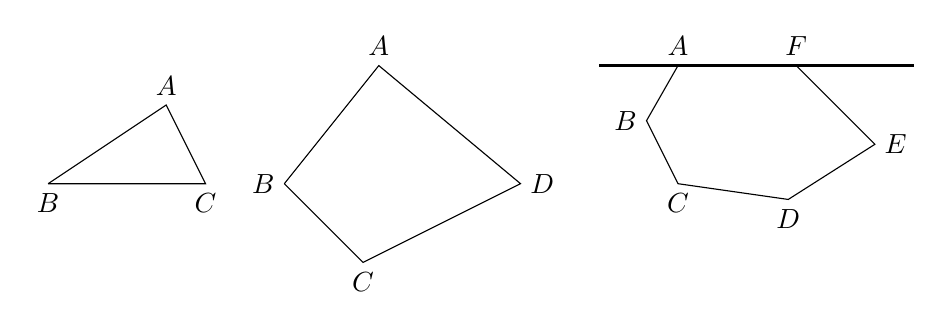
\begin{tikzpicture}
\begin{scope}
\draw(0,0)node[below]{$B$}--(2,0)node[below]{$C$}--(1.5,1)node[above]{$A$}--(0,0);
\end{scope}
\begin{scope}[xshift=3cm]
\draw (0,0)node[left]{$B$}--(1,-1)node[below]{$C$}--(3,0)node[right]{$D$}--(1.2,1.5)node[above]{$A$}--(0,0);
\end{scope}
\begin{scope}[xshift=8cm, yshift=1.5cm]
\draw (0,0)node[above]{$A$}--(1.5,0)node[above]{$F$}--(2.5,-1)node[right]{$E$}--(1.4,-1.7)node[below]{$D$}--(0,-1.5)node[below]{$C$}--(-.4,-.7)node[left]{$B$}--(0,0);
\draw[thick](-1,0)--(3,0);
\end{scope}        
    \end{tikzpicture}
    \caption{}\label{fig:3-1}
\end{figure}

\begin{figure}
    \centering
\begin{tikzpicture}
\draw[dashed](-2,0)--(2,0);
\draw (-.5,0)--(0.2,0)--(.3,-1)--(.7,1.8)--(-.5,0);
\end{tikzpicture}
    \caption{}\label{fig:3-2}
\end{figure}

\begin{Definition}{定义}
两个能够完全叠合的三角形叫做\Concept{全等三角形}。两个全等三角形完全叠合时,互相叠合的顶点叫做\Concept{对应点},互相叠合的边叫做\Concept{对应边},互相叠合的角叫做\Concept{对应角}。因此,\emph{全等三角形的对应边相等,对应角相等}。
\end{Definition}
 
怎样判定两个三角形全等呢?
\begin{enumerate}
  \item 有两边和它们的夹角对应相等的两个三角形全等。(SAS)
  \item 有两角和它们的夹边对应相等的两个三角形全等。(ASA)
  \item 有三边对应相等的两个三角形全等。(SSS)
\end{enumerate}

利用三角形的全等,是判断两条线段或两个角相等的一种基本方法。

\begin{example}
在\cref{fig:3-3} 中,已知 $\overline{AB}=\overline{AC}$,$\angle B=\angle C$,求证:$\overline{BD}=\overline{CE}$。
\end{example}

\begin{analyze}
要证 $\overline{BD}=\overline{CE}$,从图上看 $\overline{BD}$,$\overline{CE}$ 分别是 $\triangle ABD$ 和 $\triangle ACE$ 的边,因此只要证明 $\triangle ACE \cong \triangle ABD$ 就行了,由已知条件 $\overline{AC}=\overline{AB}$,$\angle B=\angle C$ 而 $\angle A$ 是公共角,所以 $\triangle ABD$ 与 $\triangle ACE$ 全等是很显然的。
\end{analyze}

\begin{proof}
在 $\triangle ABD$ 与 $\triangle ACE$ 中,

$\because\quad \overline{AB}=\overline{AC},\quad \angle B=\angle C$(已知)。

而 $\angle A=\angle A$(公共角),

$\therefore\quad \triangle ABD\cong \triangle ACE$ (ASA)。

$\therefore\quad \overline{BD}=\overline{CE}$ (全等三角形的对应边相等)。
\end{proof}    

\begin{figure}
  \begin{minipage}[b]{0.48\linewidth}
    \centering
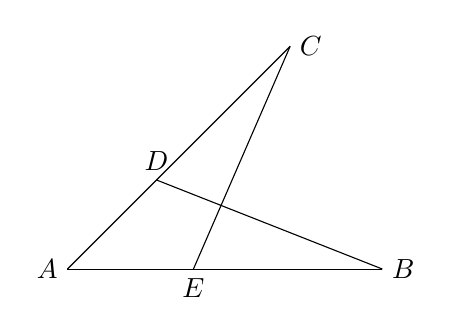
\begin{tikzpicture}[>=latex, scale=.8]
       \draw (0,0)node[left]{$A$}--(5,0)node[right]{$B$};
\draw (0,0)--(45:5)node[right]{$C$};
\draw (2,0)node[below]{$E$}--(45:5);
\draw (45:2)node[above]{$D$}--(5,0);
    \end{tikzpicture}
    \caption{}
  \end{minipage}
  \begin{minipage}[b]{0.48\linewidth}
    \centering
    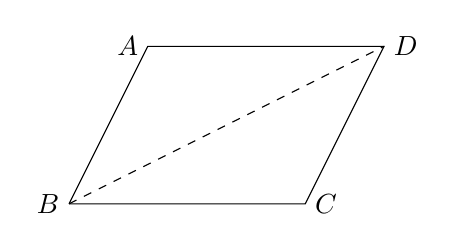
\begin{tikzpicture}[>=latex, scale=1]
        \draw (0,0)node[left]{$B$}--(3,0)node[right]{$C$}--(4,2)node[right]{$D$}--(1,2)node[left]{$A$}--(0,0);
        \draw[dashed](0,0)--(4,2);   
    \end{tikzpicture}
    \caption{}\label{fig:3-3}
  \end{minipage}
\end{figure}


\begin{example}
已知:在四边形 $ABCD$ 中,$\overline{AD}=\overline{BC}$,$\overline{AB}=\overline{CD}$(图3.4)。

求证:$\angle A=\angle C$。
\end{example}

\begin{analyze}
要证明$\angle A=\angle C$,需要把四边形 $ABCD$ 分成两个三角形,为此,连结 $B$、$D$。这叫做添\Concept{辅助线}。这样只需证 $\triangle ABD\cong \triangle CDB$ 就行了。
\end{analyze}

\begin{proof}
连结 $B$、$D$,在 $\triangle ABD$ 与 $\triangle CDB$ 中,

$\because\quad \overline{AD}=\overline{BC},\quad \overline{AB}=\overline{CD}$ (已知)

又 $\because\quad \overline{BD}=\overline{BD}$ (公共边)

$\therefore\quad \triangle ABD\cong \triangle CDB$ (SSS)

$\therefore\quad \angle A=\angle C$(全等三角形的对应角相等)。
\end{proof}    

\begin{example}
在图3.5中,已知:$\overline{AB}=\overline{CD}$,$\angle B=\angle CDF$,$\overline{BD}=\overline{EF}$。

求证:$\overline{AE}=\overline{CF}$。
\end{example}

\begin{analyze}
    要证$\overline{AE}=\overline{CF}$,只需证$\triangle ABE\cong \triangle CDF$。由已
知,$\overline{AB}=\overline{CD}$,$\angle B=\angle CDF$,$\overline{BD}=\overline{EF}$,虽然不能马上说
$\triangle ABE$和$\triangle CDF$全等,但只要注意到$\overline{BD}+\overline{DE}=\overline{DE}+\overline{EF}$,
即$\overline{EB}=\overline{DF}$就行了。
\end{analyze}

\begin{proof}
    在图3-5中,$\because\quad \overline{BD}=\overline{EF}$ 已知

$\therefore\quad \overline{BD}+\overline{DE}=\overline{DE}+\overline{EF}$ (等量加等量和相等)。即:
\[\overline{BE}=\overline{DF}\]
又$\because\quad \overline{AB}=\overline{CD},\; \angle B =\angle CDF$ 已知

$\therefore\quad \triangle ABE\cong \triangle CDF$ (SAS).

$\therefore\quad \overline{AE}=\overline{CF}$ (全等三角形的对应边相等)。
\end{proof}

\begin{figure}
    \begin{minipage}[t]{0.48\linewidth}
    \centering
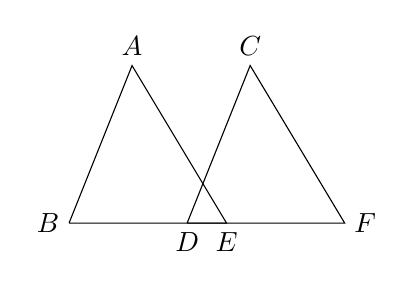
\begin{tikzpicture}[>=latex, scale=1]
       \draw(0,0)node[left]{$B$}--(2,0)node[below]{$E$}--(.8,2)node[above]{$A$}--(0,0);
\draw(1.5,0)node[below]{$D$}--(3.5,0)node[right]{$F$}--(2.3,2)node[above]{$C$}--(1.5,0);
    \end{tikzpicture}
    \caption{ }
    \end{minipage}
    \begin{minipage}[t]{0.48\linewidth}
    \centering
    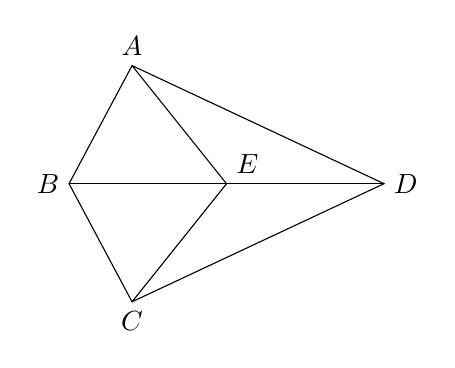
\begin{tikzpicture}[>=latex, xscale=.8]
      \draw(0,0)node[left]{$B$}--(5,0)node[right]{$D$};
      \draw(1,1.5)node[above]{$A$}--(2.5,0)node[above right]{$E$}--(1,-1.5)node[below]{$C$}--(0,0)--(1,1.5)--(5,0)--(1,-1.5);
    \end{tikzpicture}
    \caption{ }
    \end{minipage}
    \end{figure}

\begin{example}
    在图3.6中,已知:$\overline{AB}=\overline{BC}$,$\overline{AD}=\overline{CD}$,$E$点在$BD$上。

求证:$\overline{AE}=\overline{CE}$。
\end{example}

\begin{analyze}
    要证$\overline{AE}=\overline{CE}$,只需证明$\triangle ABE\cong \triangle CBE$,或者证明$\triangle ADE\cong \triangle CDE$,假定我们证明$\triangle ABE\cong \triangle CBE$,
    已知$\overline{AB}=\overline{BC}$,$\overline{BE}=\overline{BE}$,因此只需证明$\angle ABD=\angle CBD$;
    要证$\angle ABD=\angle CBD$,只需证明$\triangle ABD\cong\triangle CBD$。
\end{analyze}

\begin{proof}
    在$\triangle ABD$与$\triangle CBD$中,

    $\because\quad \overline{AB}=\overline{CB},\quad \overline{AD}=\overline{CD}$ (已知)   $\overline{BD}=\overline{BD}$(公共边)

    $\therefore\quad \triangle ABD\cong \triangle CBD$ (SSS).

    $\therefore\quad \angle ABD=\angle CBD$ (全等三角形的对应角相等)

$\because\quad     \overline{AB}=\overline{BC}$ (已知) 
    $\overline{BE}=\overline{BE}$ (公共边)

$\therefore\quad \triangle ABE\cong \triangle CBE$ (SAS).

$\therefore\quad \overline{AE}=\overline{CE}$ (全等三角形的对应边相等)。
\end{proof}

    利用三角形全等,来证明两条线段或两个角相等,关键
    在于找出能够全等的三角形,并且使要证明的线段和角恰好
    成为它们的对应边和对应角。为了找出全等的三角形,必要
    时需要添加辅助线。  

\begin{Practice}
\begin{question}
  \item 已知:在四边形 $ABCD$ 中,$AC$ 平分 $\angle BAD$,$\overline{AB}=\overline{AD}$。求证:$\angle ACB=\angle ACD$。
  \item 已知:如图,$\overline{AC}$、$\overline{BD}$ 交于 $O$ 点,且 $\overline{AO}=\overline{OC}$、$\overline{BO}=\overline{OD}$。求证:$\overline{AB}=\overline{CD}$。


\item 已知:如图,$\angle 1=\angle 4$,$\angle 2=\angle 3$。
求证:$\overline{AB}=\overline{CD}$。
\item 已知:如图,$\angle 1=\angle 2$,$\angle 3=\angle 4$,$\overline{AB}=\overline{AD}$。

求证:$\overline{AE}=\overline{AC}$,$\angle E=\angle C$。

\item 已知:如图,$\angle 1=\angle 2$,$\angle 3=\angle 4$,
求证:$\overline{AC}=\overline{BD}$。
\item 已知:如图,在四边形$ABCD$中,$\overline{AB}=\overline{BC}$,$\overline{AD}=\overline{CD}$。

求证:$\angle A=\angle C$。
\item 已知:如图,$\overline{AD}=\overline{BE}$,$\overline{AE}=\overline{BD}$,AC、BC是直线。

求证:$\angle CDB=\angle CEA$。
\item 已知:如图,$\overline{AB}=\overline{CD}$,E、F分别是$\overline{AB}$、$\overline{CD}$的中点,
并且$\overline{BF}=\overline{CE}$。

求证:$\angle EBC=\angle FCB$,$\angle FBC=\angle ECB$。

\item 已知:如图,在四边形$ABCD$中,$\overline{AB}=\overline{CD}$,$\overline{AD}=\overline{BC}$,$\overline{EF}$过$\overline{BD}$的中点$O$。

求证:$\overline{OE}=\overline{OF}$。
\end{question}
\end{Practice}

\begin{figure}
    \begin{minipage}[t]{0.48\linewidth}
    \centering
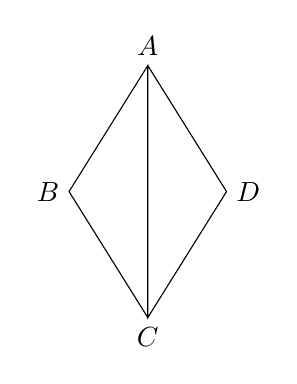
\begin{tikzpicture}[>=latex, yscale=.8]
       \draw(0,2)node[above]{$A$}--(1,0)node[right]{$D$}--(0,-2)node[below]{$C$}--(0,2)--(-1,0)node[left]{$B$}--(0,-2);
    \end{tikzpicture}
    \caption*{第1题}
    \end{minipage}
    \begin{minipage}[t]{0.48\linewidth}
    \centering
    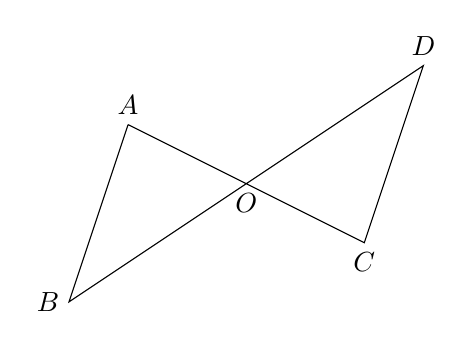
\begin{tikzpicture}[>=latex, scale=1.5]
      \draw(-1,.5)node[above]{$A$}--(1,-.5)node[below]{$C$}--(1.5,1)node[above]{$D$}--(-1.5,-1)node[left]{$B$}--(-1,.5);
      \node at (0,0)[below]{$O$};
    \end{tikzpicture}
    \caption*{第2题}
    \end{minipage}
    \end{figure}

\begin{figure}
    \begin{minipage}[t]{0.48\linewidth}
    \centering
\begin{tikzpicture}[>=latex, scale=1.3]
% \tkzDefPoints{1/2/A, 0/0/B, 3/0/C, 4/2/D}
% \tkzDrawPolygon(A,B,C)
% \tkzDrawPolygon(A,D,C)
% \tkzMarkAngle[mark=none, size=.35](B,A,C)  
% \tkzLabelAngle[pos=.5](B,A,C) {2}
% \tkzMarkAngle[mark=none, size=.5](C,A,D)  
% \tkzLabelAngle[pos=.7](C,A,D) {1}
%  \tkzLabelAngle[pos=.75](A,C,B) {4}
% \tkzMarkAngle[mark=none, size=.5](D,C,A)  
% \tkzLabelAngle[pos=.25](D,C,A) {3}
% \tkzMarkAngle[mark=none, size=.6](A,C,B) 
% \tkzLabelPoints[left](A,B)
% \tkzLabelPoints[right](C,D)
    \end{tikzpicture}
    \caption*{第3题}
    \end{minipage}
    \begin{minipage}[t]{0.48\linewidth}
    \centering
    \begin{tikzpicture}[>=latex, scale=1.3]
    % \tkzDefPoint(0,0){A}
    % \tkzDefPoint(-90:2){B}
    % \tkzDefPoint(-60:2){D}
    % \tkzDefPoint(0:2.75){E}
    % \tkzDefPoint(-30:2.75){C}
    % \tkzLabelPoints[left](A,B)
    % \tkzDrawPolygon(A,B,D)
    % \tkzDrawLines[add=0 and 1.38](B,D) %\tkzGetPoint{C}
    % \draw (D)--(E)--(A)--(C);
    % \tkzLabelPoints[right](C,E)
    % \tkzLabelPoints[below](D)
    % \tkzMarkAngles[mark=none, size=.44](C,A,E B,A,D C,B,A E,D,A)  
    % \tkzLabelAngle[pos=.65](C,A,E) {2}
    % \tkzLabelAngle[pos=.65](B,A,D) {1}
    % \tkzLabelAngle[pos=.6](C,B,A) {3}
    % \tkzLabelAngle[pos=.6](E,D,A) {4}
    \end{tikzpicture}
    \caption*{第4题}
    \end{minipage}
    \end{figure}



\begin{figure}
    \begin{minipage}[t]{0.48\linewidth}
    \centering
\begin{tikzpicture}[>=latex, scale=1]
% \tkzDefPoints{-1/2/A, 1/2/D, -2/-1/B, 2/-1/C}
% \tkzDrawPolygon(A,C,D) \tkzDrawPolygon(A,B,D)
% \tkzLabelPoints[left](A,B)
% \tkzLabelPoints[right](C,D)
% \tkzMarkAngles[mark=none, size=.6](C,A,D A,D,B) 
% \tkzMarkAngles[mark=none, size=.5](B,A,C B,D,C) 
% \tkzLabelAngle[pos=.7](C,A,D) {1}
% \tkzLabelAngle[pos=.7](A,D,B) {2}
% \tkzLabelAngle[pos=.65](B,A,C) {3}
% \tkzLabelAngle[pos=.65](B,D,C) {4}
    \end{tikzpicture}
    \caption*{第5题}
    \end{minipage}
    \begin{minipage}[t]{0.48\linewidth}
    \centering
    \begin{tikzpicture}[>=latex, scale=1.3]
        % \tkzDefPoints{-1/0/B, 2/0/D, 1/1/A, 1/-1/C, 0/0/O} 
        % \tkzDrawPolygon(A,B,C,D)
        % \tkzAutoLabelPoints[center=O](A,B,C,D)
    \end{tikzpicture}
    \caption*{第6题}
    \end{minipage}
    \end{figure}




\begin{figure}
    \begin{minipage}[t]{0.48\linewidth}
    \centering
\begin{tikzpicture}[>=latex, scale=1]
    % \tkzDefPoints{-1.5/0/A, 1.5/0/B, 0/3/C, 0/1.5/O}  
    % \tkzDefMidPoint(A,C)\tkzGetPoint{D}
    % \tkzDefMidPoint(B,C)\tkzGetPoint{E}    
    % \tkzDrawPolygon(A,B,C)
    % \draw(B)--(D)node[left]{$D$};
    % \draw (A)--(E)node[right]{$E$};
    % \tkzAutoLabelPoints[center=O](A,B,C)
    \end{tikzpicture}
    \caption*{第7题}
    \end{minipage}
    \begin{minipage}[t]{0.48\linewidth}
    \centering
    \begin{tikzpicture}[>=latex, scale=.8]
        % \tkzDefPoints{-2.5/0/B, 2.5/0/C, -1.5/3/A, 1.5/3/D,  0/1.5/O}  
        % \tkzDefMidPoint(A,B)\tkzGetPoint{E}
        % \tkzDefMidPoint(D,C)\tkzGetPoint{F}    
        % \tkzDrawPolygon(A,B,C,D)
        % \draw(B)--(F)node[right]{$F$};
        % \draw (C)--(E)node[left]{$E$};
        % \tkzAutoLabelPoints[center=O](A,B,C,D)
    \end{tikzpicture}
    \caption*{第8题}
    \end{minipage}
    \end{figure}


\begin{figure}
    \begin{minipage}[t]{0.48\linewidth}
    \centering
\begin{tikzpicture}[>=latex, scale=.8]
    % \tkzDefPoints{-2.5/0/B, 2.5/0/C, -1.5/3/A, 3.5/3/D}  
    % \tkzDefMidPoint(D,B)\tkzGetPoint{O}
    % \tkzDrawPolygon(A,B,C,D)
    % \draw (0,3)node[above]{$E$}--(1,0)node[below]{$F$};
    % \tkzAutoLabelPoints[center=O](A,B,C,D)
    % \draw(B)--(D);
    % \node at (O)[right]{$O$};

    \end{tikzpicture}
    \caption*{第9题}
    \end{minipage}
    \begin{minipage}[t]{0.48\linewidth}
    \centering
    \begin{tikzpicture}[>=latex, scale=1]
% \tkzDefPoints{-1.5/0/B, 1.5/0/C, 0/3/A, 0/1.5/O}
% \tkzDrawPolygon(A,B,C)
% \tkzAutoLabelPoints[center=O](A,B,C)
% \tkzMarkAngles[mark=none, size=.5](C,B,A A,C,B B,A,C) 
% \node at (0,-.25){底};\node at (0,2.25){顶角};
% \node at (-1,1.5){腰};\node at (1,1.5){腰};
% \node(A) at (0,.25){底角};
% \draw[<-](-1,.25)--(A);
% \draw[<-](1,.25)--(A);
    \end{tikzpicture}
    \caption{}
    \end{minipage}
    \end{figure}

\subsection{等腰三角形}

\begin{Definition}
有两条边相等的三角形叫做\Concept{等腰三角形}。相等的两边叫做\Concept{腰},另外的一边叫做\Concept{底},腰和底的夹角叫做\Concept{底角},两腰的夹角叫\Concept{顶角},如图3.7所示。
\end{Definition}

\begin{Definition}
三角形的一个角的平分线与对边相交,这个角的
顶点和交点之间的线段叫做\Concept{三角形的角的平分线}。在图
3.8(1)中,$\overline{AF}$平分$\angle A$,交对边于$F$点,$\overline{AF}$就是$\triangle ABC$
的$\angle A$的平分线。  

连结三角形一个顶点和它的对边中点的线段叫做\Concept{三角形
的中线}。在图3.8(2)中,$E$点是$\overline{BC}$的中点,$\overline{AF}$就是$\triangle ABC$的$\overline{BC}$边上的中线。

从三角形一个顶点到它的对边所在直线作垂线,顶点和
垂足之间的线段叫做\Concept{三角形的高线}(简称\Concept{高})。在图3.8(3)
中,$\overline{AD}\perp$直线$BC$,$D$是垂足,$\overline{AD}$就是$\triangle ABC$的$\overline{BC}$边上
的高线。
\end{Definition}

\begin{figure}
    \centering
\begin{tikzpicture}[scale=.8]
% \begin{scope}
% \tkzDefPoints{0/0/B, 3.6/0/F, 5.5/0/C, 4.5/3/A}
% \tkzDrawPolygon(A,B,C)
% \draw(A)--(F);
% \tkzMarkAngles[mark=none, size=.5](B,A,F) 
% \tkzMarkAngles[mark=none, size=.6](F,A,C)
% \tkzLabelAngle[pos=.7](B,A,F) {1}
% \tkzLabelAngle[pos=.75](F,A,C) {2}

% \tkzLabelPoints[below](C, F, B)
% \tkzLabelPoint(A){$A$}
% \node at (2.7,-1){(1)};
% \end{scope}
% \begin{scope}[xshift=7cm]
%     \tkzDefPoints{0/0/B, 2/0/E, 4/0/C, 4.5/3/A}
%     \tkzDrawPolygon(A,B,C)
%     \tkzLabelPoints[below](C, E, B)
%     \tkzLabelPoint(A){$A$}
%     \draw(E)--(A);
%     \node at (2.2,-1){(2)};
% \end{scope}    
% \begin{scope}[yshift=-5cm]
% \draw (0,0)node[below]{$B$}--(5.5,0)node[below]{$C$}--(4.5,3)node[above]{$A$}--(0,0);
% \tkzDefPoints{4.5/3/A1, 4.5/0/D1, 5.5/0/C1}
% \tkzMarkRightAngle(A1,D1,C1)
% \draw(4.5,3)--(4.5,0)node[below]{$D$};
% \draw(11,3)--(11,0)node[below]{$D$};
% \draw[dashed](9,0)--(12,0);
% \draw (7,0)node[below]{$B$}--(9.5,0)node[below]{$C$}--(11,3)node[above]{$A$}--(7,0);
% \tkzDefPoints{11/3/A2, 11/0/D2, 9.5/0/C2}
% \tkzMarkRightAngle(A2,D2,C2)
% \node at (6,-1){(3)};
% \end{scope}
\end{tikzpicture}
    \caption{}
\end{figure}

三角形的高线、中线、角平分线,一般是指一条线段,但有时当我们不考虑其长度时,也把它们分别所在的直线叫做三角形的高线、中线、角的平分线。


\begin{Theorem}[等腰三角形性质定理]{定理}
等腰三角形底角相等。
\end{Theorem}

已知:在 $\triangle ABC$ 中;$AB=AC$。求证:$\angle B=\angle C$。

\begin{figure}
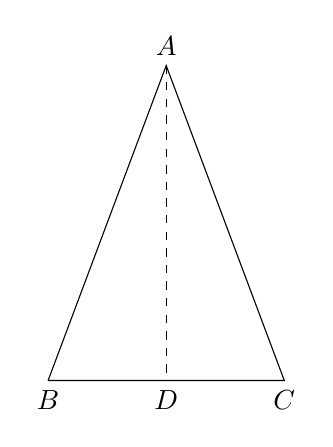
\begin{tikzpicture}
\draw (0,0)node[below]{$B$}--(3,0)node[below]{$C$}--(1.5,4)node[above]{$A$}--(0,0);
\draw[dashed](1.5,4)--(1.5,0)node[below]{$D$};
\end{tikzpicture}
    \caption{}\label{fig:3-9}
\end{figure}
\begin{proof}
作 $\angle BAC$ 的平分线 $\overline{AD}$(\cref{fig:3-9}),在 $\triangle ABD$ 和 $\triangle ACD$ 中

$\because\quad AB=AC$ (已知),$\overline{AD}=\overline{AD}$(公共边),$\angle BAD=\angle CAD$(角平分线定义)

$\therefore\quad \triangle ABD≤\triangle ACD$(SAS)

$\therefore\quad \angle B=\angle C$(全等三角形的对应角相等)。
\end{proof}


由于 $\overline{BD}=\overline{DC},\; \angle BDA=\angle CDA=\ang{90}$

因此 $AD$平分$\overline{BC}$,且$AD\perp BC$。

\begin{Deduction}{推论}
等腰三角形顶角的平分线垂直、平分底边。
\end{Deduction}

也就是说,等腰三角形的顶角平分线也是底边上的高线和中线。(\emph{三线合一})

\begin{Theorem}[等腰三角形的判定定理]{定理} 
有两个角相等的三角形是等腰三角形。
\end{Theorem}

已知:在$\triangle ABC$中,$\angle B=\angle C$(图3.10)。求证:$\overline{AB}=\overline{AC}$。

\begin{figure}
    \centering
\begin{tikzpicture}
\draw(0,0)node[left]{$B$}--(2,0)node[right]{$C$}--(1,2)node[above]{$A$}--(0,0);
\draw(4,2)node[left]{$B'$}--(6,2)node[right]{$C'$}--(5,0)node[below]{$A'$}--(4,2);
\end{tikzpicture}
    \caption{}\label{fig:3-10}
\end{figure}


\begin{proof}
    根据翻转公理,我们可以把$\triangle ABC$翻转过来,
    设顶点$A$、$B$、$C$成为$A'$、$B'$、$C'$。
    
    $\because\quad \angle B=\angle C=\angle C',\quad \angle C=\angle B=\angle B'$

    又:$\because\quad \overline{BC}=\overline{C'B'}$

    $\therefore\quad \triangle ABC\cong \triangle A'C'B'$(ASA)

    $\therefore\quad \overline{AB}=\overline{A'C'}$(全等三角形的对应边相等)。

由于$\overline{AC}=\overline{A'C'}$,$\therefore\quad \overline{AB}=\overline{AC}$(等量代换)
\end{proof}

用逻辑语句说:等腰三角形的判定定理是其性质定理的
逆定理。这两个定理我们用“充要”条件可合写成一个定理:

\begin{Theorem}{定理}
   一个三角形是等腰三角形的充要条件是这个三角形有两
个角相等。
\end{Theorem}

\begin{Definition}
三条边都相等的三角形叫做\Concept{等边三角形},也叫做\Concept{正三角形}。
\end{Definition}


同学们自己证明下面等边三角形的性质定理和判定定理。

\begin{Theorem}[等边三角形的性质定理和判定定理]{定理}
  \begin{itemize}
    \item 等边三角形的三内角相等。
    \item 三内角相等的三角形是等边三角形。
  \end{itemize}
\end{Theorem}

由等腰三角形及等边三角形的性质定理和判定定理可知,在一个三角形中,由边的相等可以推知角的相等,反过来由角的相等也可推知边的相等。下面举例说明它们在证题中的应用。

\begin{example}
已知:在图3.11中,$\overline{AB}=\overline{EB}$,$\overline{AC}=\overline{DC}$,$ADB$、$AEC$是直线。

求证:$\angle ADC=\angle AEB$。
\end{example}

\begin{analyze}
要证 $\angle ADC=\angle AEB$,只需证明 $\angle ADC=\angle A$,$\angle AEB=\angle A$; 要证明 $\angle ADC=\angle A$,$\angle AEB=\angle A$,只要知道$\overline{AC}=\overline{DC}$,$\overline{AB}=\overline{BE}$ 就行了。
\end{analyze}

\begin{proof}
在$\triangle BAE$中,$\because\quad \overline{AB}=\overline{EB}$(已知),

$\therefore\quad \angle AEB=\angle A$(等腰三角形的底角相等)。

在$\triangle CAD$中,$\because\quad \overline{AD}=\overline{DC}$(已知),

$\therefore\quad \angle ADC=\angle A$(等腰三角形的底角相等)。

$\therefore\quad \angle ADC=\angle AEB$ (等量代换)。
\end{proof}

\begin{figure}
    \begin{minipage}[t]{0.48\linewidth}
    \centering
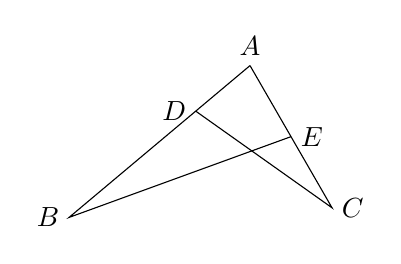
\begin{tikzpicture}[>=latex, scale=1]
\draw(40:3)node[above]{$A$}--(0,0)node[left]{$B$}--(20:3)node[right]{$E$};
\draw(40:3)--(3.34,0.122)node[right]{$C$}--(40:2.1)node[left]{$D$};
    \end{tikzpicture}
    \caption{}
    \end{minipage}
    \begin{minipage}[t]{0.48\linewidth}
    \centering
    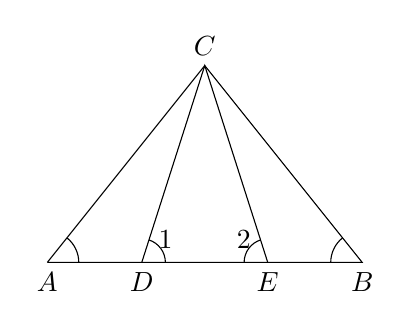
\begin{tikzpicture}[>=latex, scale=1]
\draw(-2,0)node[below]{$A$}--(0,2.5)node[above]{$C$}--(2,0)node[below]{$B$}--(-2,0);
\draw(.8,0)node[below]{$E$}--(0,2.5)--(-.8,0)node[below]{$D$};
\draw (-2+.4,0) arc (0:51.34:.4);
\draw (2-.4,0) arc (180:180-51.34:.4);
\draw (-.8+.3,0) arc (0:72.3:.3)node[right]{1};
\draw (.8-.3,0) arc (180:180-72.3:.3)node[left]{2};
    \end{tikzpicture}
    \caption{}
    \end{minipage}
    \end{figure}


\begin{example}
    如图3.12, 
己知:$\overline{AC}=\overline{BC}$,$\overline{AE}=\overline{DB}$。

求证:$\overline{CD}=\overline{CE}$。
\end{example}

\begin{analyze}
    在$\triangle CDE$中,若要证$\overline{CD}=\overline{CE}$,
   只要证$\angle 1=\angle 2$即可, $\angle 1$和$\angle 2$分别在$\triangle BCD$与$\triangle ACE$中,如能证明$\triangle BCD\cong \triangle ACE$,即可证明$\angle 1=\angle 2$。
\end{analyze}

\begin{solution}
在$\triangle ACE$与$\triangle BCD$中,

$\because\quad \overline{AC}=\overline{BC},\quad \overline{AE}=\overline{BD}$ (已知)

$\therefore\quad \angle A=\angle B$(等腰三角形两底角相等),

$\therefore\quad \triangle ACE\cong \triangle BCD$(SAS)

$\therefore\quad \angle 2=\angle 1$(全等三角形的对应角相等),

$\therefore\quad \triangle CDE$ 是等腰三角形(有两角相等的三角形是等腰三角形)。

$\therefore\quad \overline{CD}=\overline{CE}$
\end{solution}

\begin{Practice}
\begin{question}
\item\label{prac:3-2-1} 画出 $\triangle ABC$ 和 $\triangle DEF$ 的三条边上的高线。
\begin{figurehere}
  \begin{minipage}{\linewidth}\centering
    % 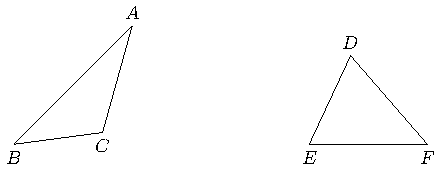
\includegraphics{pr3-2-1.pdf}
    \caption*{第 \ref{prac:3-2-1} 题}
  \end{minipage}
\end{figurehere}
\item 画一个三角形 $ABC$,然后画出 $\triangle ABC$ 三个内角的平分线。
\item 画一个三角形 $DEF$,然后画出 $\triangle DEF$ 三边上的中线。
\item 证明:全等三角形的对应角的平分线相等。
\item 证明:全等三角形对应边上的中线相等。
\item 已知:$A=\{\text{等腰三角形}\}$,$B=\{\text{两内角相等的三角形}\}$,指出集合 $A$ 与集合 $B$ 的关系。
\item\label{prac:3-2-7} 若 $\overline{AC}=\overline{BC},\quad \angle DCA=\angle ECB$,则 $\overline{CD}=\overline{CE}$。
\item\label{prac:3-2-8} 若 $\overline{AC}=\overline{BC},\quad \angle 1=\angle 2$,则 $\overline{AE}=\overline{BD}$。
\begin{figurehere}
  \begin{minipage}[b]{0.45\linewidth}\centering
    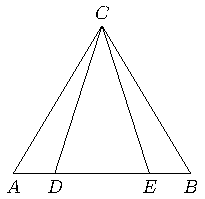
\includegraphics{pr3-2-7.pdf}
    \caption*{第 \ref{prac:3-2-7} 题}
  \end{minipage}
  \begin{minipage}[b]{0.45\linewidth}\centering
    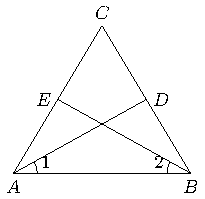
\includegraphics{pr3-2-89.pdf}
    \caption*{第 \ref{prac:3-2-8}--\ref{prac:3-2-9} 题}
  \end{minipage}
\end{figurehere}
\item\label{prac:3-2-9} 若 $\overline{AC}=\overline{BC}$,$\overline{AD}$、$\overline{BE}$ 分别是 $\angle A$ 和 $\angle B$ 的平分线,则 $\overline{AD}=\overline{BE}$。
\item 若 $\overline{AC}=\overline{BC},\quad \overline{AD}=\overline{BE}$,$DE$ 是直线,则 $\triangle DEC$ 是等腰三角形。
\item 若 $\overline{AC}=\overline{BC},\quad \angle ACD=\angle BCE$,$DE$ 是直线,则 $\triangle DEC$ 是等腰三角形。
\item 在等边 $\triangle ABC$ 的三边上,分别取 $D$、$E$、$F$(如图),使 $\overline{AD}=\overline{BE}=\overline{CF}$,则 $\triangle DEF$ 是等边三角形。
\item 设 $\overline{DE}=\overline{EF}=\overline{FD}$,$\angle AFD=\angle BDE=\angle CEF$,则 $\triangle ABC$ 是等边三角形。
\end{question}
\end{Practice}

\begin{figure}
    \begin{minipage}[t]{0.48\linewidth}
    \centering
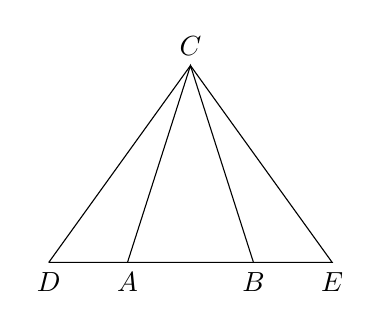
\begin{tikzpicture}[>=latex, scale=1]
    \draw(-1.8,0)node[below]{$D$}--(0,2.5)node[above]{$C$}--(1.8,0)node[below]{$E$}--(-1.8,0);
    \draw(.8,0)node[below]{$B$}--(0,2.5)--(-.8,0)node[below]{$A$};
    \end{tikzpicture}
    \caption*{第10--11题}
    \end{minipage}
    \begin{minipage}[t]{0.48\linewidth}
    \centering
    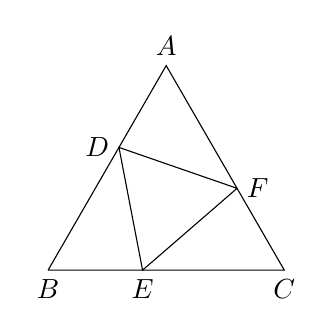
\begin{tikzpicture}[>=latex, scale=1]
\draw(-120:3)node[below]{$B$} --(0,0)node[above]{$A$}--(-60:3)node[below]{$C$}-- (-120:3) ;
\draw(-60:1.8)node[right]{$F$}--(-120:1.2)node[left]{$D$}--(-.3,-1.5*1.732)node[below]{$E$}--(-60:1.8);
    \end{tikzpicture}
    \caption*{第12--13题}
    \end{minipage}
    \end{figure}

\subsection{轴对称图形}
\begin{Definition}
在平面上有两个图形 $F$ 和 $F'$,如果平面沿着某条直线 $\ell$ 折叠起来,$F$ 和 $F'$ 叠合,就称 $F$ 和 $F'$ 关于 $\ell$ 成\Concept{轴对称}。(也称 $F$ 和 $F'$ 是以 $\ell$ 为轴的\Concept{对称形})。$F$ 和 $F'$ 上互相叠合的点叫做\Concept{对称点},$\ell$ 叫做\Concept{对称轴}。
\end{Definition}

在图3.13(1)中,平面上的 $\triangle ABC$ 和 $\triangle A'B'C'$ 关于直线 $\ell$ 成轴对称;$A$与$A'$、$B$ 与 $B'$、$C$ 与 $C'$ 都是对称点。

\begin{figure}
\begin{tikzpicture}
\begin{scope}
    \draw(0,-.5)--(0,4)node[above]{$\ell$};
    \node at (0,-1){(1)};
\draw(-1.8,2)node[above]{$B$}--(-.4,3)node[above]{$A$}--(-1.4,0.5)node[below]{$C$}--(-1.8,2);
\draw(1.8,2)node[above]{$B'$}--(.4,3)node[above]{$A'$}--(1.4,0.5)node[below]{$C'$}--(1.8,2);
\end{scope}
\begin{scope}[xshift=6.5cm]
    \draw(0,-.5)--(0,4)node[above]{$\ell$};
\draw(-2,0)node[below]{$B$}--(2,0)node[below]{$C$}--(0,3)node[right]{$A$}--(-2,0);
\draw (0,0) rectangle (.2,.2);
\node at (0,-1){(2)};
\end{scope}
\end{tikzpicture}
    \caption{}\label{fig:3-13}
\end{figure}

\begin{Deduction}{推论}
两个图形如果关于某直线成轴对称,那么这两个图形是全等形。
\end{Deduction}

\begin{Definition}
如果一个图形可以分成两部分,这两部分关于某一直线成轴对称,就把这个图形称为\Concept{轴对称形}。
\end{Definition}

显然,等腰三角形关于它的顶角平分线成轴对称图形图3.13(2))。轴对称形在实际中应用非常广泛,图3.14中的图形,都是轴对称形。
\begin{figure}
% \includegraphics[scale=.6]{fig/3-14.png}
    \caption{}\label{fig:3-14}
\end{figure}

轴对称图形有什么性质呢?这就要研究一下对称轴和对称点的关系。

在图3.15中,设 $A$ 与 $A'$ 是关于直线 $\ell$ 的轴对称点,因为 $A$、$A'$和$\ell$在同一平面内,并且 $A$ 和 $A'$ 在 $\ell$ 的两侧,所以线段 $\overline{AA'}$ 与 $\ell$ 必相交,设交点为 $O$,在 $\ell$ 上取异于 $O$的另一点$P$,连结 $\overline{AP}$,$\overline{A'P}$。

由于 $A$ 点所在的半平面沿直线 $\ell$ 折叠过来,$A$ 和 $A'$ 重合,而 $\ell$ 上的 $P$ 和 $O$ 重合于自身,所以$\overline{AP}=\overline{A'P}$,$\angle APO=\angle A'PO$,$\triangle PAA'$是等腰三角形,直线$\ell$是顶角的平分线,
所以 $\ell$ 垂直平分底边 $\overline{AA'}$。

由此得出轴对称图形的重要性质:
\begin{enumerate}
  \item 对称轴上的任一点,与每一双对称点的距离相等。
  \item 对称轴是每一双对称点所连线段的垂直平分线。
\end{enumerate}

在上述性质的证明中,我们所取 $P$ 点异于 $O$,如果 $P$ 点就是 $O$ 点,结论仍然一样。

由于一条线段的垂直平分线是唯一的,由性质2可知,如果 $\overline{AA'}$ 的垂直平分线是 $\ell$,那么 $A$ 与 $A'$ 是以 $\ell$ 为轴的对称点。

由此,我们就可以作出已知图形以某直线为轴的对称形。

\begin{figure}
    \begin{minipage}[t]{0.48\linewidth}
    \centering
\begin{tikzpicture}[>=latex, scale=.8]
    \draw(0,-.5)--(0,4)node[above]{$\ell$};
\draw(-2,0)node[below]{$A$}--(2,0)node[below]{$A'$}--(0,3)node[right]{$P$}--(-2,0);
\draw (0,0)node[below right]{$O$} rectangle (.2,.2);
    \end{tikzpicture}
    \caption{}
    \end{minipage}
    \begin{minipage}[t]{0.48\linewidth}
    \centering
    \begin{tikzpicture}[>=latex, scale=1]
% \draw(0,-.5)--(0,4)node[above]{$\ell$};     
% \tkzDefPoints{-1/3/A, 1/3/A', -2.5/2/B,2.5/2/B',-1.5/0/C,1.5/0/C',-.5/.8/D, .5/.8/D'}
% \tkzDrawPolygon(A,B,C,D)\tkzDrawPolygon(A',B',C',D')
% \foreach \x in {A,B,C,D}
% {
%     \draw(\x)--(\x');
% }
% \tkzDefPoints{0/2.1/O}
% \tkzAutoLabelPoints[center=O](A,B,C,D,A',B',C',D')
% \node at (0,3)[below right]{$O$};
% \draw(0,3) rectangle (-.2,3+.2);
    \end{tikzpicture}
    \caption{}
    \end{minipage}
    \end{figure}



\begin{example}
已知:四边形$ABCD$及直线$\ell$。(图3.16)

求作:四边形$ABCD$以$\ell$为轴的轴对称形。

作法:
\begin{enumerate}
\item 由$A$点引$\ell$的垂线交$\ell$于$O$点,在射线$AO$上
取$OA'=AO$,则$A'$是$A$点关于轴$\ell$的对称点。
\item 用同样的方法作点$B$、$C$、$D$关于$\ell$的对称点$B'$、
$C'$、$D'$。
\item 连结$\overline{A'B'}$,$\overline{B'C'}$,$\overline{C'D'}$,$\overline{D'A'}$,则四边形
$A'B'C'D'$就是四边形$ABCD$以$\ell$为轴的轴对称图形。
\end{enumerate}

为什么呢?因为根据作法,如果把四边形 $ABCD$ 和四边形 $A'B'C'D'$ 所在平面,沿直线$\ell$折叠起来,则 $A$ 与 $A'$、
$B$与$B'$、$C$与$C'$、$D$与$D'$分别重合,所以四边形$ABCD$与
四边形$A'B'C'D'$完全重合,所以这两个四边形是以$\ell$为轴
的对称图形。
\end{example}

\begin{example}
    有公共底的两个等腰三角形,通过底所对的两个顶点的直线是它们所组成图形的对称轴。

已知:在图3.17中,$BC$是等腰$\triangle ABC$与等腰$\triangle A'BC$
的公共底边。

求证:直线$AA'$是这个图形的对称轴。
\end{example}

\begin{figure}
    \centering
\begin{tikzpicture}[scale=.8]
\begin{scope}
\draw(0,-1.5)--(0,4);
\draw(-1.5,0)node[left]{$B$}--(1.5,0)node[right]{$C$}--(0,3)node[right]{$A$}--(-1.5,0)--(0,-1)node[right]{$A'$}--(1.5,0);

\end{scope}
\begin{scope}[xshift=7cm]
    \draw(0,-1)--(0,4);
\draw(-1.5,0)node[left]{$B$}--(1.5,0)node[right]{$C$}--(0,3)node[right]{$A$}--(-1.5,0)--(0,1.8)node[right]{$A'$}--(1.5,0);

\end{scope}
\end{tikzpicture}
    \caption{}
\end{figure}

\begin{proof}
$\because\quad \overline{AB}=\overline{AC},\quad \overline{A'B}=\overline{A'C}$(已知)

$\therefore\quad \angle ABC=\angle ACB,\quad 
\angle A'BC=\angle A'CB$(等腰三角形的两底角相等)。

两式相加(或相减)得:
$\angle ABA'=\angle ACA'$(等量加(或减)等量其和(或差)
相等)。

$\therefore\quad \triangle ABA'\cong \triangle ACA'$(SAS)

以$AA'$为轴折叠起来,$\triangle ABA'$与$\triangle ACA'$能够重
合,所以$AA'$是这个图形的对称轴。
\end{proof}

\begin{example}
    证明四条边相等的四边形的两条对角线互相垂直
平分,并且平分一双对角。

已知:在四边形$ABCD$中,$\overline{AB}=\overline{BC}=\overline{CD}=\overline{DA}$。
(图3.18)
\begin{figure}
    \centering
    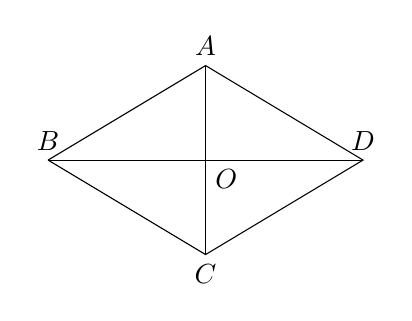
\begin{tikzpicture}
    \draw(-2,0)--(0,1.2)--(2,0)--(0,-1.2)--(-2,0);
    \draw(-2,0)node[above]{$B$}--(2,0)node[above]{$D$};
    \draw(0,1.2)node[above]{$A$}--(0,-1.2)node[below]{$C$};
    \node at (0,0)[below right]{$O$};        
    \end{tikzpicture}
    \caption{}
\end{figure}

求证:$AC$、$BD$互相垂直平分,且$AC$平分$\angle A$和$\angle C$,
$BD$平分$\angle B$和$\angle D$。
\end{example}

\begin{proof}
在四边形$ABCD$中,
因为$\overline{AB}=\overline{BC}=\overline{CD}=\overline{DA}$,所
以四边形$ABCD$可看成由两个
等腰三角形所拼成:等腰$\triangle ABD$
与等腰$\triangle CBD$,或等腰$\triangle ABC$
与等腰$\triangle ADC$。由例3.8可知,
对角线$\overline{AC}$、$\overline{BD}$所在的直线都是四边形$ABCD$的对称
轴。所以,$\overline{AC}$、$\overline{BD}$互相垂直平分,并且$\overline{AC}$平分$\angle A$和
$\angle C$,$\overline{BD}$平分$\angle B$和$\angle D$。
\end{proof}

\begin{Practice}
\begin{question}
  \item 下列各图形有多少个对称轴?对称轴是什么?
  \begin{tasks}(3)
    \task 线段;
    \task 射线;
    \task 直线。
  \end{tasks}
  \item 已知直线 $\ell$ 和 $\ell$ 外面一点 $A$,只用圆规和直尺求作点 $A$ 以直线 $\ell$ 为对称轴的对称点 $A'$。
  \item 求作两个已知点的对称轴。
  \item 已知 $\triangle ABC$ 和直线 $\ell$,作 $\triangle ABC$ 以 $\ell$ 为对称轴的对称形。
  \item 求作与已知等边三角形 $ABC$ 分别以 $AB$、$AC$、$BC$ 为对称轴的对称图形。
  \item 作图。(只要求作出图形)
  \begin{tasks}(2)
    \task 画已知线段 $\overline{AB}$ 的对称轴。
    \task 画已知 $\angle A$ 的对称轴。
  \end{tasks}
  \item 等腰三角形有几个对称轴?等边三角形有几个对称轴?任画一个等边三角形把它的对称轴都画出来。
\end{question}
\end{Practice}

\subsection{三角形中的不等关系}
\begin{Definition}
    和三角形的内角相邻并且和它互补的角叫做三角
形的\Concept{外角}。
\end{Definition}
 
如图3.19中的$\angle ACD$
就是$\triangle ABC$的一外个角。
这时$\angle ACB$称为$\angle ACD$
相邻的内角,$\angle A$和$\angle B$
分别称为$\angle ACD$不相邻的内角。

\begin{Theorem}{定理}
 三角形的外角大于和它不相邻的任一内角。
\end{Theorem}

\begin{figure}
    \begin{minipage}[t]{0.48\linewidth}
    \centering
\begin{tikzpicture}[>=latex, scale=1]
\draw(0,0)node[left]{$B$}--(4.5,0)node[right]{$D$};
\draw(3,0)node[below]{$C$}--(1.7,2)node[above]{$A$}--(0,0);
\draw(3.4,0) arc (0:120:.4);
    \end{tikzpicture}
    \caption{}
    \end{minipage}
    \begin{minipage}[t]{0.48\linewidth}
    \centering
    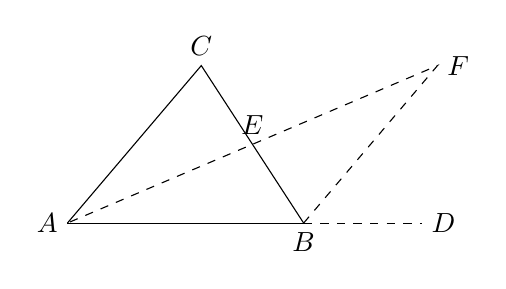
\begin{tikzpicture}[>=latex, scale=1]
\draw(0,0)node[left]{$A$}--(3,0)node[below]{$B$};
\draw[dashed](3,0)--(4.5,0)node[right]{$D$};
\draw(3,0)--(1.7,2)node[above]{$C$}--(0,0);
\draw[dashed](3,0)--(4.7,2)node[right]{$F$}--(0,0); 
\node at (2.35,1)[above]{$E$};
    \end{tikzpicture}
    \caption{}
    \end{minipage}
    \end{figure}

已知:$\triangle ABC$和外角
$\angle CBD$(图3.20)。

求证:$\angle CBD>\angle C$
或$\angle A$。

\begin{proof}
    假定$E$是$\overline{BC}$
中点,引$AE$并延长到$F$,
使$\overline{EF}=\overline{AE}$,作$\overline{BF}$。

在$\triangle ACE$和$\triangle FBE$中,

$\because\quad \overline{AE}=\overline{EF}$ (作图),

$\because\quad E$是$\overline{BC}$中点(假定),

$\therefore\quad \overline{CE}=\overline{EB}$(线段中点定义),

$\because\quad \angle CEA=\angle BEF$(对顶角相等),

$\therefore\quad \triangle ACE\cong \triangle FBE$ (SAS),

$\therefore\quad \angle EBF=\angle C$(全等三角形的对应角相等)。

由于$\angle CBD>\angle EBF$ (全量大于它的任何一部分)。

$\therefore\quad \angle CBD>\angle C$ (等量代换)。

同理可证 $\angle CBD> \angle A$。
\end{proof}

\begin{Theorem}{定理}
 在一个三角形中,如果两条边不等,那么它们所
对的角也不等,大边所对的角较大;反之,如果在一个三角
形中两个角不等,那么它们所对的边也不等。大角所对的边
较大。
\end{Theorem}

已知:$\triangle ABC$(图3.21)

\begin{figure}
    \begin{minipage}[t]{0.48\linewidth}
    \centering
\begin{tikzpicture}[>=latex, scale=1.3]
% \tkzDefPoint(0,0){A}
% \tkzDefPoint(-50:2){C}
% \tkzDefPoint(-120:2){D}
% \tkzDefPoint(-120:3){B}
% \tkzDefPoint(0,-1.5){O}
% \tkzDrawPolygon(A,C,B)
% \draw[dashed](D)--(C);
% \tkzMarkAngles[mark=none, size=.3](C,D,A A,C,D)
% \tkzLabelAngle[pos=.6](C,D,A){2}
% \tkzLabelAngle[pos=.6](A,C,D){1}
% \tkzAutoLabelPoints[center=O](A,C,B,D)       
    \end{tikzpicture}
    \caption{}
    \end{minipage}
    \begin{minipage}[t]{0.48\linewidth}
    \centering
    \begin{tikzpicture}[>=latex, scale=1.3]
% \tkzDefPoint(0,0){A}
% \tkzDefPoint(30:1.5){D}
% \tkzDefPoint(-150:2){B}
% \tkzDefPoint(-30:1.5){C}
% \tkzDrawPolygon(A,C,B)
% \draw[dashed](A)--(D)--(C);
% \tkzMarkAngles[mark=none, size=.2](D,C,A A,D,C)
% \tkzLabelAngle[pos=.4](A,D,C){2}
% \tkzLabelAngle[pos=.4](D,C,A){1}
% \tkzAutoLabelPoints[center=A](C,B,D)  
% \node at (0,0)[above left]{$A$};
    \end{tikzpicture}
    \caption{}
    \end{minipage}
    \end{figure}

求证:
\begin{enumerate}
    \item $\overline{AB}>\overline{AC}\quad \Rightarrow\quad \angle C>\angle B$
    \item $\angle C>\angle B\quad \Rightarrow\quad \overline{AB}>\overline{AC}$
\end{enumerate}

\begin{proof}
    先证$\overline{AB}>\overline{AC}\quad\Rightarrow\quad \angle C>\angle B$。

在$AB$上截$\overline{AD}=\overline{AC}$,
则$\triangle ADC$为等腰三角形。

$\therefore\quad \angle 1=\angle 2$。

由于$\angle ACB>\angle 1$ (不等量基本性质6)

$\therefore\quad \angle ACB>\angle 2$(等量代换)。

但$\angle 2>\angle B$ (三角形的外角大于和它不相邻的任一内
角),

$\therefore\quad \angle ACB>\angle B$(不等量基本性质5)

即:$\angle C>\angle B$。

我们再证$\angle C>\angle B\quad \Rightarrow\quad \overline{AB}>\overline{AC}$

如果$\overline{AB}$不大于$\overline{AC}$,那么$\overline{AB}=\overline{AC}$或$\overline{AB}<\overline{AC}$。
若$\overline{AB}=\overline{AC}$,则$\angle B=\angle C$,若$\overline{AB}<\overline{AC}$,则$\angle C<\angle B$,这两
种结果都和$\angle C>\angle B$矛盾。

$\therefore\quad \angle C>\angle B\quad \Rightarrow\quad \overline{AB}>\overline{AC}$
\end{proof}

\begin{Theorem}{定理}
    三角形任意两边之和大于第三边。
\end{Theorem}
 
已知:$\triangle ABC$(图3.23)。

求证:$\overline{AB}+\overline{AC}>\overline{BC}$。

\begin{proof}
    在$BA$的延长线上取一点$D$,使$AD=AC$。则
    $\triangle ACD$为等腰三角形。
  
    $\therefore\quad \angle 1=\angle 2$

    $\because\quad \angle BCD>\angle 1$(不等量
    基本性质6)

$\therefore\quad \angle BCD>\angle 2$(等量代
    换)。

    在$\triangle BCD$中,由前面的定理可知:
    $\overline{BD}>\overline{BC}$,但$\overline{BD}=\overline{AB}+\overline{AD}=\overline{AB}+\overline{AC}$,
 
   $\therefore\quad  \overline{AB}+\overline{AC}>\overline{BC}$
\end{proof}

\begin{Deduction}{推论}
三角形任一边大于其他两边之差。
\end{Deduction}

下面我们举例说明上述定理的一些应用。


\begin{example}
    已知:$\triangle ABC$中$\overline{AB}=\overline{AC}$,$D$点在$\overline{BC}$上,$E$点
在$\overline{BC}$的延长线上(图3.23)。

求证:$\overline{AD}<\overline{AB}<\overline{AE}$
\end{example}

\begin{figure}
    \begin{minipage}[t]{0.48\linewidth}
    \centering
\begin{tikzpicture}[>=latex, scale=1]
%     \tkzDefPoints{0/1.5/A, -1.5/-1/B, -.25/-1/D, 1.5/-1/C, 2.5/-1/E}
% \tkzDrawPolygon(A,C,B)
%     \draw(D)node[below]{$D$}--(A)node[above]{$A$}--(E)node[below]{$E$};
% \draw[dashed](C)--(3.5,-1);
% \node at (B)[below]{$B$};
% \node at (C)[below]{$C$};
% \tkzMarkAngles[mark=none, size=.3](D,B,A  A,D,B  A,C,B)
% \tkzLabelAngle[pos=.5](D,B,A){1}
% \tkzLabelAngle[pos=.5](A,D,B){3}
% \tkzLabelAngle[pos=.5](A,C,B){2}
    \end{tikzpicture}
    \caption{}
    \end{minipage}
    \begin{minipage}[t]{0.48\linewidth}
    \centering
    \begin{tikzpicture}[>=latex, scale=1.2]
% \tkzDefPoint(0,0){D}
% \tkzDefPoint(-60:2){C}
% \tkzDefPoint(180-60:1){A}
% \tkzDefPoint(-140:1.2){E}
% \tkzDefPoint(-140:2.8){B}
% \tkzDrawPolygon(A,C,B)
% \draw(B)--(E)--(C);
% \draw[dashed](E)--(D);
% \foreach \x in {A,D,C}
% {
%     \node at (\x) [right]{ $\times$ };
% }
% \foreach \x in {B,E}
% {
%     \node at (\x) [left]{ $\times$ };
% }
% \tkzMarkAngles[mark=none, size=.2](E,D,C)
% \tkzLabelAngle[pos=.4](E,D,C){1}
    \end{tikzpicture}
    \caption{}
    \end{minipage}
    \end{figure}

\begin{proof}
$\because\quad \overline{AB}=\overline{AC}$

$\therefore\quad \angle 1=\angle 2$

又$\because\quad \angle 3>\angle 2$

$\therefore\quad \angle 3>\angle 1$

$\therefore\quad \overline{AB}>\overline{AD}$(在一个三角形中,大角对大边。)

又:$\because\quad \angle 2>\angle E$

$\therefore\quad \angle 1>\angle E$

$\therefore\quad \overline{AE}>\overline{AB}$(在一个三角形中,大角对大边。)

因此有:$\overline{AD}<\overline{AB}<\overline{AE}$
\end{proof}


\begin{example}
    已知:$E$点在$\triangle ABC$内(图3.24)。

求证: \begin{enumerate}
    \item $\angle BEC>\angle A$
    \item $\overline{BE}+\overline{EC}<\overline{AB}+\overline{AC}$
\end{enumerate} 
\end{example}

\begin{proof}
    延长$\overline{BE}$交$\overline{AC}$于$D$点,
则$\angle BEC>\angle 1$,$\angle BEC>\angle 1$

$\therefore\quad \angle BEC>\angle A$(不等量基
本性质5)。

又$\because\quad \overline{BE}+\overline{ED}<\overline{AD}+\overline{AB}$,$\overline{EC}<\overline{ED}+\overline{DC}$(三角形两边之和大于第三边)。

$\therefore\quad \overline{BE}+\overline{ED}+\overline{EC}<\overline{AD}+\overline{AB}+\overline{ED}+\overline{DC}$(不等量基本性质3)。

$\therefore\quad \overline{BE}+\overline{EC}<\overline{AB}+\overline{AC}$(不等量基本性质1)。
\end{proof}

\begin{example}
如图3.25所示,$A$、$B$是平面上直线$\ell$同侧的两点,试在直线$\ell$上求一点$P$,使$\overline{AP}+\overline{PB}$最短。

在没有作这题前,让我们想一想该怎样着手,我们要求$\overline{AP}+\overline{PB}$最短,但怎样才能最短呢?

我们知道两点间的直线段最短,但是我们却要在$\ell$上求一点,使$\overline{AP}+\overline{PB}$最短。如果$A,B$两点在$\ell$的两侧,那么问题要简单得多(作$\overline{AB}$与$\ell$交于$P$,$P$点就是所求的点)。但我们曾学过,如果两点是轴对称点,那么它们的对称轴就是两点间线段的垂直平分线,并且对称轴上的点到两对称点的距离相等。我们只要作出$A$点关于轴$\ell$的对称点$A'$,我们求$\overline{AP}+\overline{PB}$的最小值,就可转化为求$\overline{A'P}+\overline{PB}$的最小值了。而$A'$、$B$两点在$\ell$的异侧,这是很容易的。

\begin{figure}
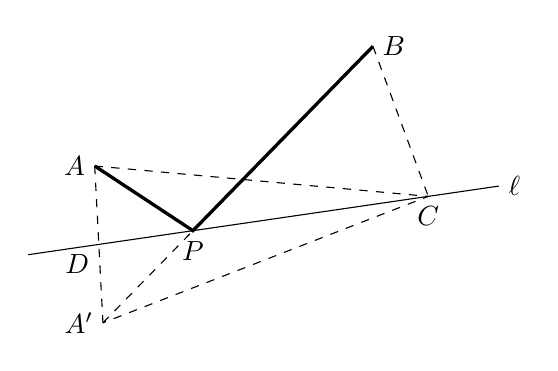
\begin{tikzpicture}[xscale=.6, rotate=5]
\draw (-2,0)--(8,0)node[right]{$\ell$};
\draw[dashed](-.5,1)node[left]{$A$}--(-.5,-1)node[left]{$A'$};
\draw[dashed](-.5,-1)--(5.5,2)node[right]{$B$};
\draw[very thick](-.5,1)--(1.5,0)node[below]{$P$}--(5.5,2);
\node at (-.5,0)[below left]{$D$};
\draw[dashed](-.5,1)  -- (6.5,0) node[below]{$C$}--(-.5,-1);
\draw[dashed](5.5,2)  -- (6.5,0);
\end{tikzpicture}
    \caption{}
\end{figure}
\end{example}


\begin{solution}
    作$A$点关于轴$\ell$的对称点$A'$,作$\overline{A'B}$与$\ell$相交于$P$,
    则$P$点使$\overline{AP}+\overline{PB}$最短。因为,如果在$\ell$上任找另外一点$C$,
    在$\triangle A'BC$中,
    $\overline{A'B}<\overline{A'C}+\overline{CB}$(三角形两边之和大于第三边),
    但$\overline{A'B}=\overline{A'P}+\overline{PB}$

将    $\overline{A'P}=\overline{AP},\quad \overline{A'C}=\overline{AC}$ 代入上式,
    则得:$\overline{AP}+\overline{PB}<\overline{AC}+\overline{CB}$。

    这就证明了$P$点使$\overline{AP}+\overline{PB}$最短。
\end{solution}

\begin{rmk}
    如果$\ell$是镜子的话,那么从$A$点发出的光线,若反
射到$B$点,那么$\overline{AP}$、$\overline{PB}$就是光所走的路线。因为光线总是
走最近的路,在光学中就有:“入射角等于反射角”这条定
律。即$\angle APD=\angle BPC$。在光学中由观测得到的结果和我
们用数学定理得出的结果一致。在自然界中我们有能力观测
到的结论是有限的,如何由这些有限的可观测的结论,得到
更进一步的结论,甚至有些是观测不到的结论,我们需要数
学这样有力的工具。
\end{rmk}
    
\begin{Practice}
\begin{question}
  \item 已知:如图,$\triangle ABC$ 内有一点 $P$,求证:$\angle BPC>\angle BAC$。
  \item 已知:如图,$\triangle ABC$ 内有一点 $P$,求证:$\overline{AB}+\overline{AC}>\overline{PB}+\overline{PC}$。
  \item 将金属丝弯成三角形,如果要求一边长是 \qty{25}{cm},那么金属丝至少大于多少 \unit{cm} 才能作成三角形?
  \item 证明四边形两条对角线之和小于周长而大于半周长。
  \item 证明三角形的一边小于它的周长的一半。
  \item 用整数表示三角形的各边,一边是 \qty{3}{m},另一边是 \qty{2}{m},第三边可以是多少米?
  \item 在平面上 $\overline{AB}$ 的垂直平分线的 $A$ 点的一侧取一点 $P$,那么 $\overline{PA}$ 和 $\overline{PB}$ 哪一条线段长?
  \item 已知:如图,$\triangle ABC$ 中,$\angle A>\angle C$,$D$、$E$ 分别在 $\overline{AB}$、$\overline{AC}$ 上并且 $\overline{AD}>\overline{AE}$。求证:
  \begin{tasks}
    \task $\angle BDE> \angle CED$
    \task $\overline{BC}>\overline{BE}$
  \end{tasks}
\end{question}
\end{Practice}
    
\begin{figure}
    \begin{minipage}[t]{0.48\linewidth}
    \centering
\begin{tikzpicture}[>=latex, scale=1]
%     \tkzDefPoint(-60:2){C}
%     \tkzDefPoint(180-60:1){A}
%     \tkzDefPoint(-140:2.8){B}
%     \tkzDefPoint(-.25,-.5){P}
%     \tkzDrawPolygon(A,C,B)
%     \draw(B)--(P)--(C);
% \tkzAutoLabelPoints[center=P](A,B,C)
% \node at (P)[above]{$P$};
    \end{tikzpicture}
    \caption*{第1--2题}
    \end{minipage}
    \begin{minipage}[t]{0.48\linewidth}
    \centering
    \begin{tikzpicture}[>=latex, scale=1.3]
        % \tkzDefPoint(0,0){A}
        % \tkzDefPoint(-45:2){C}
        % \tkzDefPoint(-45:1){E}
        % \tkzDefPoint(-140:2.8){B}
        % \tkzDefPoint(-140:2){D}
        % \tkzDrawPolygon(A,C,B)
        % \tkzDrawPolygon(D,B,E)
        % \tkzDefPoint(.1,-1){O}
        % \tkzAutoLabelPoints[center=O](A,B,C,D,E)
    \end{tikzpicture}
    \caption*{第8题}
    \end{minipage}
    \end{figure}

\section*{习题3.1}
\addcontentsline{toc}{subsection}{习题3.1}
\begin{enumerate}
    \item 已知:如图,$\overline{AD}=\overline{AE}$,$\overline{BD}=\overline{EC}$,
    求证:$\overline{DO}=\overline{EO}$。
    \item 已知:如图,$\overline{AB}=\overline{AD}$,$AC$平分$\angle BAD$,$E$是$\overline{AC}$上一点。
    求证:$\angle EBC=\angle EDC$。
    \item 求证:等腰三角形两腰上的中线相等。
    \item 已知:如图,$\angle B=\angle C$,$\overline{BD}=\overline{EC}$。
    求证:$\angle 1=\angle 2$。

\begin{figure}
    \begin{minipage}[t]{0.31\linewidth}
    \centering
\begin{tikzpicture}[>=latex, scale=1]
% \tkzDefPoints{-1.5/0/B, 1.5/0/C, -.5/2/D, .5/2/E, 0/3/A}
% \tkzDrawPolygon(A,B,C)
% \tkzDrawSegments(B,E C,D)
% \tkzInterLL(C,D)(B,E)  \tkzGetPoint{O}
% \tkzLabelPoints[left](B,D)
% \tkzLabelPoints[right](C,E)
% \tkzLabelPoints[above](A)
% \tkzLabelPoints[below](O)


    \end{tikzpicture}
    \caption*{第1题}
    \end{minipage}
    \begin{minipage}[t]{0.31\linewidth}
    \centering
    \begin{tikzpicture}[>=latex, scale=1]
% \tkzDefPoints{-1.5/0/B, 1.5/0/D, 0/1.5/A, 0/-2/C, 0/.8/E}
% \tkzDrawPolygon(A,B,C,D)
% \tkzDrawSegments(B,E A,C E,D)
% \tkzLabelPoints[left](B)
% \tkzLabelPoints[right](D)
% \tkzLabelPoints[above](A)
% \tkzLabelPoints[below](C)
% \tkzLabelPoints[below right](E)
    \end{tikzpicture}
    \caption*{第2题}
    \end{minipage}
        \begin{minipage}[t]{0.31\linewidth}
    \centering
    \begin{tikzpicture}[>=latex, scale=1]
% \tkzDefPoints{-1.5/0/B, 1.5/0/C, -.75/0/D, .75/0/E, 0/3/A}
% \tkzDrawPolygon(A,B,C)
% \tkzDrawSegments(A,E A,D)
% \tkzLabelPoints[left](B)
% \tkzLabelPoints[right](C)
% \tkzLabelPoints[above](A)
% \tkzLabelPoints[below](D,E)
% \tkzMarkAngles[mark=none, size=.3](C,D,A A,E,B)
% \tkzLabelAngle[pos=.5](C,D,A){1}
% \tkzLabelAngle[pos=.5](A,E,B){2}
    \end{tikzpicture}
    \caption*{第4题}
    \end{minipage}
    \end{figure}

    \item 已知:如图,在四边形$ABCD$中,
    $\overline{AD}=\overline{AB}$,$\overline{CD}=\overline{BC}$
    
    求证:$\angle 1=\angle 2$;$\angle 3=\angle 4$;$AC\perp DB$
  
    \item 如图,已知:$\angle 1=\angle 2$,$\angle 3=\angle 4$,
求证:$\overline{AB}=\overline{AC}$。
\item 如图,已知:$\overline{BE}=\overline{ED}$,$\angle 1=\angle 2$。
求证:$\overline{AB}=\overline{CD}$。

\begin{figure}
    \begin{minipage}[t]{0.48\linewidth}
    \centering
\begin{tikzpicture}[>=latex, scale=1]
    % \tkzDefPoints{-2/0/A, 2/0/C, -1/1.5/D, -1/-1.5/B, -1/0/E}
    % \tkzDrawPolygon(A,B,C,D)
    % \tkzLabelPoints[left](A)
    % \tkzLabelPoints[right](C)
    % \tkzLabelPoints[above](D)
    % \tkzLabelPoints[below](B)
    % \tkzLabelPoints[above right](E)
    % \tkzDrawSegments(A,C D,B)
    % \tkzMarkAngles[mark=none, size=.4](C,A,D D,C,A)
    % \tkzMarkAngles[mark=none, size=.5](B,A,C A,C,B)
    % \tkzLabelAngle[pos=.7](C,A,D){1}
    % \tkzLabelAngle[pos=.7](B,A,C){2}
    % \tkzLabelAngle[pos=.7](D,C,A){3}
    % \tkzLabelAngle[pos=.7](A,C,B){4}

    \end{tikzpicture}
    \caption*{第5题}
    \end{minipage}
    \begin{minipage}[t]{0.48\linewidth}
    \centering
    \begin{tikzpicture}[>=latex, scale=1]
        % \tkzDefPoints{-1.5/0/B, 1.5/0/C, 0/3.5/A, 0/1/O}
        % \tkzDrawPolygon(A,B,C)
        % \tkzLabelPoints[left](B)
        % \tkzLabelPoints[right](C)
        % \tkzLabelPoints[above](A)
        % \tkzLabelPoints[below](O)
        % \tkzDrawSegments(A,O B,O C,O)        
        % \tkzMarkAngles[mark=none, size=.4](C,B,O O,C,B)
        % \tkzMarkAngles[mark=none, size=.3](A,O,B)
        % \tkzLabelAngle[pos=.6](C,B,O){1}
        % \tkzLabelAngle[pos=.6](O,C,B){2}
        % \tkzLabelAngle[pos=.5](A,O,B){3}
        % \tkzMarkAngles[mark=none, size=.35](C,O,A)
        % \tkzLabelAngle[pos=.5](C,O,A){4}

    \end{tikzpicture}
    \caption*{第6题}
    \end{minipage}
    \end{figure}

\item 在 $\triangle ABC$ 中,$\overline{AB}=\overline{AC}$,$D$、$E$ 两点分别在 $\overline{AB}$ 和 $\overline{AC}$ 上,且 $\overline{BE}$
和$\overline{CD}$交于$O$点,$\overline{BD}=\overline{CE}$。求证:$AO$平分$\angle BAC$。
\item 在$\triangle ABC$中,$D$为$\overline{BC}$延长线上一点,且$\overline{CD}=\overline{AC}$,$F$
是
$\overline{AD}$中点,$\overline{CE}$是$\angle ACB$的平分线。求证$CE\perp CF$。

\item 在$\triangle ABC$中,$\angle B=2\angle C$,$AD$平分$\angle A$,交$\overline{BC}$于$D$点,
求证:$\overline{AB}+\overline{BD}=\overline{AC}$。

\begin{figure}
    \begin{minipage}[t]{0.48\linewidth}
    \centering
\begin{tikzpicture}[>=latex, scale=1]
    % \tkzDefPoints{-1.5/0/A, 1.5/0/C, -1/2/B, 1/2/D}
    % \tkzDrawPolygon(A,B,C)
    % \tkzDrawPolygon(A,D,C)
    % \tkzInterLL(B,C)(A,D) \tkzGetPoint{E}
    % \tkzLabelPoints[left](A)
    % \tkzLabelPoints[right](C)
    % \tkzLabelPoints[above](B,D,E)
    % \tkzMarkAngles[mark=none, size=.4](B,C,A C,A,D)
    % \tkzLabelAngle[pos=.6](C,A,D){1}
    % \tkzLabelAngle[pos=.6](B,C,A){2}
    \end{tikzpicture}
    \caption*{第7题}
    \end{minipage}
    \begin{minipage}[t]{0.48\linewidth}
    \centering
    \begin{tikzpicture}[>=latex, scale=1]
% \tkzDefPoints{0/0/B, 3/0/C, 3/1.5/D}
% \tkzDefPoint(70:3){A}
% \tkzDrawPolygon(A,B,C,D)
% \tkzLabelPoints[below](B,C)
% \tkzLabelPoints[above](A,D)
    \end{tikzpicture}
    \caption*{第11题}
    \end{minipage}
    \end{figure}

\item 如图,已知四边形$ABCD$中,
$\overline{AB}=\overline{BC}$,$\overline{AD}>\overline{CD}$。

求证:$\angle BCD>\angle BAD$。
\item 已知:$\triangle ABC$中,$D$是$\overline{AC}$上
一点,且$\overline{BD}>\overline{BC}$。

求证:$\overline{AB}>\overline{AC}$。
\item 三角形的一边等于2米,另一边等于8米,如果已知第三边能用被3整除的整数表示,求第三边。
\item 已知:$\triangle ABC$在平面$\alpha$上,点$P\in\alpha$,并且$P$在$\triangle ABC$的外部

求证:$\overline{PA}+\overline{PB}+\overline{PC}>\frac{1}{2}(\overline{AB}+\overline{BC}+\overline{AC})$
\item 已知:$\triangle ABC$在平面$\alpha$上,点$P\in\alpha$,并且$P$在$\triangle ABC$的内部

求证:$\overline{PA}+\overline{PB}+\overline{PC}<\overline{AB}+\overline{BC}+\overline{AC}$。
\item 求证:三角形一边上的中线小于其他两边和的一半。
\item 在两条公路$OX$和$OY$上,分别设邮筒$A$和$B$,邮递员每天由邮局$P$到邮筒$A$、$B$取信,然后返回邮局。问$A$、$B$的位置确定在哪儿,才能使邮递员走的路程最短?

\begin{figure}[htbp]
    \centering
\begin{tikzpicture}
% \tkzDefPoints{-2/0/X, 2/0/Y, .5/3/X1, -.5/3/Y1, 0/0/P}
% \tkzDefPointWith[linear, K=.5](X,X1) \tkzGetPoint{A}
% \tkzDefPointWith[linear, K=.3](Y,Y1) \tkzGetPoint{B}
% \tkzDrawPolygon(A,B,P)
% \tkzInterLL(X,X1)(Y,Y1)  \tkzGetPoint{O}
% \tkzDrawSegments(X,X1 Y,Y1)
% \tkzLabelPoints[below](X,Y,P)
% \tkzLabelPoints[left](A)
% \tkzLabelPoints[right](B,O)
\end{tikzpicture}
    \caption*{第17题}
\end{figure}
\end{enumerate}

\section{平行线与内角和定理}

\subsection{平行线}
\begin{Definition}
平面上两条直线被第三条直线所截,截得八个
角,如图3.26, 其中的$\angle 1$和$\angle 5$,$\angle 4$和$\angle 8$,$\angle 2$和$\angle 6$,
$\angle 3$和$\angle 7$,都叫做\Concept{同位角},$\angle 4$和$\angle 6$,$\angle 3$和$\angle 5$都叫\Concept{内错
角},$\angle 4$和$\angle 5$,$\angle 3$和$\angle 6$都叫做\Concept{同旁内角}。
\end{Definition}

\begin{figure}
    \begin{minipage}[t]{0.48\linewidth}
    \centering
\begin{tikzpicture}[>=latex, scale=1]
% \tkzDefPoints{-2/2/A, 2/2.5/B, -2/0/C, 2/1.5/D, 0/-.5/F, 0/4/E}
% \tkzDrawSegments(A,B C,D E,F)
% \tkzInterLL(A,B)(E,F)  \tkzGetPoint{P}
% \tkzInterLL(C,D)(E,F)  \tkzGetPoint{Q}
% \tkzMarkAngles[mark=none, size=.4](B,P,E A,P,F D,Q,E C,Q,F)
% \tkzLabelAngle[pos=.6](B,P,E){1}
% \tkzLabelAngle[pos=.6](A,P,F){3}
% \tkzLabelAngle[pos=.6](D,Q,E){5}
% \tkzLabelAngle[pos=.6](C,Q,F){7}
% \tkzMarkAngles[mark=none, size=.3](E,P,A F,P,B E,Q,C F,Q,D)
% \tkzLabelAngle[pos=.5](E,P,A){2}
% \tkzLabelAngle[pos=.5](F,P,B){4}
% \tkzLabelAngle[pos=.5](E,Q,C){6}
% \tkzLabelAngle[pos=.5](F,Q,D){8}
    \end{tikzpicture}
    \caption{}
    \end{minipage}
    \begin{minipage}[t]{0.48\linewidth}
    \centering
    \begin{tikzpicture}[>=latex, scale=1]
% \tkzDefPoints{-2/2/A, 2/2/B, -2/0/C, 2/0/D, -1/-1/F, 1/3/E}
% \tkzDrawSegments(A,B C,D E,F)
% \tkzInterLL(A,B)(E,F)  \tkzGetPoint{P}
% \tkzInterLL(C,D)(E,F)  \tkzGetPoint{Q}
% \tkzMarkAngles[mark=none, size=.4](B,P,E A,P,F)
% \tkzLabelAngle[pos=.6](B,P,E){4}
% \tkzLabelAngle[pos=.6](A,P,F){3}
% \tkzLabelAngle[pos=.6](D,Q,E){2}
% \tkzMarkAngles[mark=none, size=.3](F,P,B D,Q,E)
% \tkzLabelAngle[pos=.5](F,P,B){1}
% \tkzLabelPoints[above](A,B,C,D)
% \tkzLabelPoints[below](Q)
% \tkzLabelPoints[above left](P)
    \end{tikzpicture}
    \caption{}
    \end{minipage}
    \end{figure}


由平行线定义可知,两条直线平行的充要条件是这两条直线被第三条直线所截出的同位角相等。这就是说:
\begin{enumerate}
\item 如果同位角相等,则两条直线平行;   
\item 如果已知两条直线平行,则同位角相等。 
\end{enumerate}
这就是平行线的判定方法和平行线的性质。以此为根据又可推知以下定理:

\begin{Theorem}{定理}
两条直线被第三条直所线截,如果内错角相等,或同旁内角互补,那么这两条直线平行。
\end{Theorem}

\begin{proof}
   在图3.27中,设直线$AB$、$CD$被直线$PQ$所截。$\angle 2$、$\angle 3$是内错角,$\angle 1$、$\angle 2$是同旁内角。
\begin{enumerate}
    \item 如果已知$\angle 2=\angle 3$。

$\because\quad \angle 3=\angle 4$    (对顶角相等),

$\therefore\quad \angle 2=\angle 4$(等量代换)。

$\therefore\quad AB\parallel CD$(同位角相等,则两条直线平行)。

\item 如果已知$\angle 1+\angle 2=\ang{180}$,
则$\angle 2=\ang{180}-\angle 1$(等量减等量差相等)。

$\because\quad PQ$是直线(已知)

$\therefore\quad \angle 4+\angle 1=\ang{180}$。

$\therefore\quad \angle 4=\ang{180}-\angle 1$。

$\therefore\quad \angle 2=\angle 4$(等量代换)。

$\therefore\quad AB\parallel CD$(同位角相等,则两条直线平行)。  
\end{enumerate}
\end{proof}

\begin{Theorem}{定理} 
    平面上两条不相交的直线是这两条直线互相平行
的充要条件。
\end{Theorem}

但是这个定理的证明比较麻烦,我们在这里就不证了,有兴趣的同学可以自己去证明它。

\begin{Deduction}{推论1} 
平行于同一直线的两条直线平行。 
\end{Deduction}

已知:直线$a\parallel$直线$c$,直线$b\parallel$直线$c$ (图3.28). 求证:$a\parallel b$。

\begin{proof}
    若$a$不平行$b$,$a$与$b$一定相交,设交点为$P$,那么
过$P$点就有两条直线$a$、$b$平行于直线$c$,但根据平行公理,
这是不可能的,所以$a\parallel b$。
\end{proof}

\begin{figure}
\begin{tikzpicture}
\begin{scope}
    \foreach \x/\xtext in {0/c,1/b,2/a}
    {
        \draw(0,\x)--node[above]{$\xtext$}(3,\x);
    }
\end{scope}
\begin{scope}[xshift=5cm]
    \foreach \x/\xtext in {0/c,1/b,2/a}
    {
        \draw(0,\x)--node[above]{$\xtext$}(3,\x);
    }
\draw[dashed](3,1)--(4.5,1.5)node[right]{$P$}--(3,2);
\end{scope}
\end{tikzpicture}
    \caption{}
\end{figure}


上面这种证明方法,叫做反证法。我们先否定要证明的结论,然后引出不合理的结果,从而说明结论非成立不可。请同学们回想一下,我们在第二章讲基本逻辑语句的命题时,若原命题是“若$\alpha$,则$\beta$”,那么它的逆否命题是“若非$\beta$,则非$\alpha$。”我们知道这两个互为逆否的命题是同义的,上面的反证法就是当我们证明原命题有困难时,我们可去证它的逆否命题。

\begin{Deduction}{推论2} 
  过已知直线外一点,只可以引一条直线和已知直线垂直。   
\end{Deduction}

请同学们用反证法证明这个推论。

\begin{example}
已知:在图3.29中,$\angle BED=\angle B+\angle D$。

求证:$AB\parallel CD$。
\end{example}

\begin{analyze}
若能证明 $AB$、$CD$ 都与第三条直线平行,则 $AB\parallel CD$。
\end{analyze}

\begin{proof}
引直线$EF$,使得$\angle 1=\angle B$,则$AB\parallel EF$(内错角相等,则两条直线平行)。

又:$\because\quad \angle BED=\angle B+\angle D$(已知),

$\therefore\quad \angle BED-\angle 1=\angle D$(等量减等量差相等)。即:$\angle FED=\angle D$。

$\therefore\quad CD\parallel EF$ (内错角相等,则两条直线平行)。

$\therefore\quad AB\parallel CD$ (平行于第三条直线的两条直线平
行)。
\end{proof}

\begin{figure}
  \begin{minipage}[t]{0.48\linewidth}
    \centering
\begin{tikzpicture}[>=latex, scale=1]
% \tkzDefPoints{0/0/C, 3/0/D, 2/1/E, 3/2/B, 0/2/A, 4/1/F}
% \tkzDrawSegments(C,D D,E E,B A,B)
% \tkzDrawSegments[dashed](E,F)
% \tkzLabelPoints[below](C,D)
% \tkzLabelPoints[above](A,B)
% \tkzLabelPoints[left](E)
% \tkzLabelPoints[right](F)
% \tkzMarkAngles[mark=none, size=.4](F,E,B)
% \tkzLabelAngle[pos=.6](F,E,B){1}
    \end{tikzpicture}
    \caption{}
    \end{minipage}
    \begin{minipage}[t]{0.48\linewidth}
    \centering
    \begin{tikzpicture}[>=latex, scale=1]
% \tkzDefPoints{-.25/-.25/B, .25/.25/C, 1/-.25/F, -1/.25/E, 1.5/1.5/D, -1.5/-1.5/A}
% \tkzDrawPolygon(A,E,C)
% \tkzDrawPolygon(B,F,D)
% \tkzLabelPoints[below](A,B,F)
% \tkzLabelPoints[above](E,D,C)
% \tkzMarkAngles[mark=none, size=.4](F,B,D E,C,A)
% \tkzLabelAngle[pos=.6](F,B,D){2}
% \tkzLabelAngle[pos=.6](E,C,A){1}
    \end{tikzpicture}
    \caption{}
  \end{minipage}
\end{figure}

\begin{example}
    在图3.30中,已知$\overline{CD}=\overline{AB}$,$AD$是直线。
$\angle A=\angle D$,并且$\overline{AE}=\overline{DE}$。

求证:$EC\parallel BF$。

\end{example}

\begin{analyze}
要证$EC\parallel BF$,只需证明$\angle 1=\angle 2$即可,要证明
$\angle 1=\angle 2$,只需证明$\triangle AEC\cong \triangle DFB$即可。
\end{analyze}

\begin{proof}
    $\because\quad \overline{AB}=\overline{CD}$(已知)
    $\therefore\quad \overline{AB}+\overline{BC}=\overline{BC}+\overline{CD}$(等量加等量和相等)。即:$\overline{AC}=\overline{BD}$。

又:$\because\quad \angle A=\angle D,\quad \overline{AE}=\overline{DF}$(已知),

$\therefore\quad \triangle AEC\cong \triangle DFB$ (SAS).

$\therefore\quad \angle 1=\angle 2$(全等三角形的对应角相等)。

$\therefore\quad CE\parallel BF$(内错角相等,则两条直线平行)。
\end{proof}

\begin{Theorem}
  {定理} 如果两条平行直线被一条直线所截,那么截出的
内错角相等;同旁内角互补。  
\end{Theorem}

这个定理同学们可以根据“两条直线平行则同位角相
等”这一性质推出。

\begin{example}
     在图3.31中,
已知:$OA\parallel O'A'$,$OB\parallel O'B'$。

求证:$\angle AOB=\angle A'O'B'$。  
\end{example}

\begin{proof}
    反向延长$O'A'$交$OB$于$C$点,

$\because\quad OB\parallel O'B'$(已知),

$\therefore\quad\angle A'O'B'=\angle A'CB$(两条直线平行,同位角相等)。

又$\because\quad OA\parallel O'A'$(已知),

$\therefore\quad \angle A'CB=\angle AOB$(两条直线平行,同位角相等)。

$\therefore\quad \angle AOB=\angle A'O'B'$(等量代换)。
\end{proof}

\begin{figure}
    \begin{minipage}[t]{0.48\linewidth}
    \centering
\begin{tikzpicture}[>=latex, scale=1, rotate=-20]
% \tkzDefPoints{0/0/O, 4/0/A, 2.5/1.5/O', 4.5/1.5/A', 0/1.5/C', 2.5+1.414/1.5+1.414/B', 2.5/2.5/B, 1.5/1.5/C}
% \tkzDrawSegments(A,O A',O' B,O B',O')
% \tkzDrawSegments[dashed](O',C')
% \tkzLabelPoints[below](O,A,O',A')
% \tkzLabelPoints[above](C,B,B')

    \end{tikzpicture}
    \caption{}
    \end{minipage}
    \begin{minipage}[t]{0.48\linewidth}
    \centering
    \begin{tikzpicture}[>=latex, scale=1]
% \tkzDefPoints{0/0/B, 3/0/C, 1/2/A, 4/2/D}
% \tkzDrawPolygon(A,B,C,D)
% \tkzDrawSegments(A,C)
% \tkzLabelPoints[left](A,B)\tkzLabelPoints[right](C,D)

% \tkzMarkAngles[mark=none, size=.4](A,C,B C,A,D)
% \tkzMarkAngles[mark=none, size=.3](B,A,C D,C,A)
% \tkzLabelAngle[pos=.6](A,C,B){2}
% \tkzLabelAngle[pos=.6](C,A,D){1}
% \tkzLabelAngle[pos=.5](B,A,C){3}
% \tkzLabelAngle[pos=.5](D,C,A){4}
    \end{tikzpicture}
    \caption{}
    \end{minipage}
    \end{figure}

上面的例子我们可以写成下面的定理:

\begin{Theorem}
    {定理} 如果一个角的两条边和另一个角的两条边分别同
向平行,那么这两个角相等。
\end{Theorem}

\begin{example}
    图3.32中,
    已知:$AD\parallel BC$,$\overline{AD}=\overline{BC}$。

    求证:$AB\parallel CD$。
\end{example}

\begin{analyze}
    要证明$AB\parallel CD$,只要证明$\angle 3=\angle 4$就行
了,为此需要证明$\triangle ABC\cong \triangle CDA$。
\end{analyze}

\begin{proof}
$\because\quad AD\parallel BC$(已知),

$\therefore\quad \angle 1=\angle 2$(两条直线平行,则
内错角相等)。

又:$\because\quad \overline{AD}=\overline{BC}$(已知)
$\overline{AC}=\overline{AC}$(公共边)

$\therefore\quad \triangle ABC\cong \triangle CDA$ (SAS)

$\therefore\quad \angle  3=\angle 4$(全等三角形的对应角相等)。

$\therefore\quad AB\parallel CD$(内错角相等,则两条直线平行)。
\end{proof}

\begin{Practice}
\begin{enumerate}
    \item 指出图中用数字标出的角中哪些是同位角?
    \item 如图,说出下列各对角的名称。
    $\angle 1$与$\angle 2$,$\angle 2$与$\angle 3$,$\angle 3$与$\angle 4$,$\angle 4$与$\angle 5$,$\angle 3$与
    $\angle 5$,$\angle 1$与$\angle 6$
    \item 试指出判定两条直线平行有哪些方法?并指出平行线
    有什么性质?
    \item 如图,已知:$\angle 1=\ang{60}$,$\angle 2=\ang{60}$。
    求证:$AB\parallel CD$。

    \item 如图,已知:$\angle 1=\angle 2$,求证:$AB\parallel CD$。
    \item 知图,已知$\angle 1=69^{\circ}$,$\angle 2=69^{\circ}$。
    求证:$AB\parallel CD$。
    \item 如图,已知:$\angle 1+\angle 2=\ang{180}$,求证:$AB\parallel CD$。
    \item 如图,已知:$\overline{AB}$、$\overline{CD}$相交于$E$点,且$\overline{EA}=\overline{EB}$,$\overline{EC}=\overline{ED}$
    
求证:$AC\parallel DB$。

\item 如图,已知:$\overline{AB}=\overline{DC}$,$\overline{AD}=\overline{BC}$。求证:$AB\parallel CD$。
\item 已知:$\overline{AE}=\overline{DF}$,$\overline{AB}=\overline{CD}$,$\overline{EC}=\overline{BF}$。
求证:$EC\parallel BF$。
\item 已知:$DE\parallel BC$,$\angle 1=\angle 2$。求证:$\angle 3=\angle 4$。
\item 已知:$AB\parallel CD$,求证:$\angle 1=\angle 2$。
\item 如图,已如:$\angle 1=\angle 2$。求证:$\angle 3=\angle 4$。
\item 如图,已知:$AB\parallel CD$,
求证:$\angle B+\angle D+\angle E=3\ang{60}$。

\item 在四边形$ABCD$中,$AD\parallel BC$,$AB\parallel CD$且$\overline{BE}=\overline{DF}$,则$\overline{AE}\parallel \overline{FC}$。
\end{enumerate}
\end{Practice}

\begin{figure}
    \begin{minipage}[t]{0.48\linewidth}
    \centering
\begin{tikzpicture}[>=latex, scale=1]
% \tkzDefPoints{0/0/A, 4/1/B, 0/1.5/C, 4/2.5/D, 2/-.5/F, 2/3.5/E}
% \tkzDrawSegments(A,B C,D E,F)
% \tkzInterLL(A,B)(E,F)  \tkzGetPoint{X1}
% \tkzInterLL(C,D)(E,F)  \tkzGetPoint{X2}
% \tkzDefPoints{3.5/2/Y1, 3.5/3.5/Y2}
% \tkzDrawSegments(X1,Y1 X2,Y2)
% \tkzMarkAngles[mark=none, size=.45](B,X1,Y1 D,X2,Y2)
% \tkzLabelAngle[pos=.6](B,X1,Y1){4}  \tkzLabelAngle[pos=.6](D,X2,Y2){3}
% \tkzMarkAngles[mark=none, size=.35](Y1,X1,E Y2,X2,E)
% \tkzLabelAngle[pos=.6](Y1,X1,E){2}  \tkzLabelAngle[pos=.6](Y2,X2,E){1}
    \end{tikzpicture}
    \caption*{第1题}
    \end{minipage}
    \begin{minipage}[t]{0.48\linewidth}
    \centering
    \begin{tikzpicture}[>=latex, scale=1]
%  \tkzDefPoints{0/0/A, 4/.8/B, 1.5/-1/C, 4/-.5/D, 0/2.5/E, 1.5/2.5/F}
%  \tkzDrawSegments(A,B C,D A,E C,F)
%  \tkzInterLL(A,B)(C,F)  \tkzGetPoint{G}     
%  \tkzMarkAngles[mark=none, size=.3](B,A,E D,C,F B,G,F A,G,C)
%  \tkzLabelAngle[pos=.5](B,A,E){1}  \tkzLabelAngle[pos=.5](D,C,F){4}
%  \tkzLabelAngle[pos=.5](B,G,F){2} \tkzLabelAngle[pos=.5](A,G,C){3}
%  \tkzMarkAngles[mark=none, size=.25](C,G,B F,G,A)
%  \tkzLabelAngle[pos=.4](C,G,B){5}  \tkzLabelAngle[pos=.4](F,G,A){6}
    \end{tikzpicture}
    \caption*{第2题}
    \end{minipage}
    \end{figure}



\begin{figure}
    \begin{minipage}[t]{0.32\linewidth}
    \centering
\begin{tikzpicture}[>=latex, scale=1]
%     \tkzDefPoints{0/0/C, 2.5/0/D, 0/1/A, 2.5/1/B, .5/-1/E, 2.25/2.25/F}
% \tkzInterLL(A,B)(E,F) \tkzGetPoint{X1}
% \tkzInterLL(C,D)(E,F) \tkzGetPoint{X2}
% \tkzLabelPoints[left](A,C)\tkzLabelPoints[right](B,D)
% \tkzDrawSegments(A,B C,D E,F)
% \tkzMarkAngles[mark=none, size=.4](A,X1,E C,X2,E)
% \tkzLabelAngle[pos=.6](A,X1,E){1}  \tkzLabelAngle[pos=.6](C,X2,E){2}
    \end{tikzpicture}
    \caption*{第4题}
    \end{minipage}
    \begin{minipage}[t]{0.32\linewidth}
    \centering
    \begin{tikzpicture}[>=latex, scale=1]
% \tkzDefPoints{0/0/C, 2.5/0/D, 0/1/A, 2.5/1/B, .5/-1/E, 2.25/2.25/F}
% \tkzInterLL(A,B)(E,F) \tkzGetPoint{X1}
% \tkzInterLL(C,D)(E,F) \tkzGetPoint{X2}
% \tkzLabelPoints[left](A,C)\tkzLabelPoints[right](B,D)
% \tkzDrawSegments(A,B C,D E,F)
% \tkzMarkAngles[mark=none, size=.4](B,X1,F C,X2,E)
% \tkzLabelAngle[pos=.6](B,X1,F){1}  \tkzLabelAngle[pos=.6](C,X2,E){2}
    \end{tikzpicture}
    \caption*{第5、7、12题}
    \end{minipage}
    \begin{minipage}[t]{0.32\linewidth}
    \centering
    \begin{tikzpicture}[>=latex, scale=1]
%  \tkzDefPoints{0/0/C, 2.5/0/D, 0/1/A, 2.5/1/B, .5/-1/E, 2.25/2.25/F}
% \tkzInterLL(A,B)(E,F) \tkzGetPoint{X1}
% \tkzInterLL(C,D)(E,F) \tkzGetPoint{X2}
% \tkzLabelPoints[left](A,C)\tkzLabelPoints[right](B,D)
% \tkzDrawSegments(A,B C,D E,F)
% \tkzMarkAngles[mark=none, size=.4](B,X1,F E,X2,D)
% \tkzLabelAngle[pos=.6](B,X1,F){1}  \tkzLabelAngle[pos=.6](E,X2,D){2}
    \end{tikzpicture}
    \caption*{第6题}
    \end{minipage}
    \end{figure}

\begin{figure}
    \begin{minipage}[t]{0.32\linewidth}
    \centering
\begin{tikzpicture}[>=latex, scale=1]
% \tkzDefPoints{0/0/D, 2.5/0/B, -.5/1.5/A, 2/1.5/C}
% \tkzInterLL(A,B)(C,D) \tkzGetPoint{E}
% \tkzDrawPolygon(A,C,E)
% \tkzDrawPolygon(B,D,E)
% \tkzLabelPoints[above](A,C)
% \tkzLabelPoints[below](B,D,E)
    \end{tikzpicture}
    \caption*{第8题}
    \end{minipage}
    \begin{minipage}[t]{0.32\linewidth}
    \centering
    \begin{tikzpicture}[>=latex, scale=1]
% \tkzDefPoints{0/0/B, 2.5/0/C, .75/1.5/A, 3.25/1.5/D}
% \tkzDrawPolygon(A,B,C,D)
% \tkzLabelPoints[above](A,D)
% \tkzLabelPoints[below](B,C)
    \end{tikzpicture}
    \caption*{第9题}
    \end{minipage}
    \begin{minipage}[t]{0.32\linewidth}
        \centering
        \begin{tikzpicture}[>=latex, scale=1]
% \tkzDefPoints{0/0/A, 1/0/B,2/0/C,3/0/D, .5/1/E, 2.5/-1/F}
% \tkzDrawPolygon(A,C,E)
% \tkzDrawPolygon(B,D,F)
% \tkzLabelPoints[above](E,D)
% \tkzLabelPoints[below](A,B,C,F)
        \end{tikzpicture}
        \caption*{第10题}
        \end{minipage}
    \end{figure}



    \begin{figure}
        \begin{minipage}[t]{0.46\linewidth}
        \centering
    \begin{tikzpicture}[>=latex, scale=.8]
% \tkzDefPoints{0/0/B, 4/0/C, 2.2/4/A}
% \tkzDefPointWith[linear, K=.6](A,B) \tkzGetPoint{D}
% \tkzDefPointWith[linear, K=.6](A,C) \tkzGetPoint{E}
% \tkzDrawPolygon(A,B,C)
% \tkzDrawSegments(D,E)
% \tkzLabelPoints[left](B,D)
% \tkzLabelPoints[right](C,E)
% \tkzLabelPoints[above](A)
% \tkzMarkAngles[mark=none, size=.4](E,D,A C,B,A A,C,B A,E,D)
% \tkzLabelAngle[pos=.6](E,D,A){3}  \tkzLabelAngle[pos=.6](C,B,A){1}
% \tkzLabelAngle[pos=.6](A,C,B){2}  \tkzLabelAngle[pos=.6](A,E,D){4}
        \end{tikzpicture}
        \caption*{第11题}
        \end{minipage}
        \begin{minipage}[t]{0.46\linewidth}
        \centering
        \begin{tikzpicture}[>=latex, scale=1]
%  \tkzDefPoints{0/0/C, 3/0/D, 0/1/A, 3/1/B, .5/-1/E, 1.5/2/F, 2.5/-1/G, 2/2/H}
%  \tkzDrawSegments(A,B C,D E,F G,H)
% \tkzLabelPoints[left](A,C)\tkzLabelPoints[right](B,D)
% \tkzInterLL(A,B)(E,F) \tkzGetPoint{X1}
% \tkzInterLL(C,D)(E,F) \tkzGetPoint{X2}
% \tkzInterLL(A,B)(G,H) \tkzGetPoint{Y1}
% \tkzInterLL(C,D)(G,H) \tkzGetPoint{Y2}

% \tkzMarkAngles[mark=none, size=.25](A,X1,E D,X2,F G,Y1,B G,Y2,D)
% \tkzLabelAngle[pos=.4](G,Y1,B){3}  \tkzLabelAngle[pos=.4](A,X1,E){1}
% \tkzLabelAngle[pos=.4](D,X2,F){2}  \tkzLabelAngle[pos=.4](G,Y2,D){4}
        \end{tikzpicture}
        \caption*{第13题}
        \end{minipage}

        \end{figure}

    \begin{figure}
        \begin{minipage}[t]{0.46\linewidth}
        \centering
    \begin{tikzpicture}[>=latex, scale=1]
% \tkzDefPoints{0/0/C, 2.5/0/D, 0/1.5/A, 3/1.5/B, 4/1/E}
% \tkzLabelPoints[above](A,B)
% \tkzLabelPoints[below](C,D)
% \tkzLabelPoints[right](E)
% \tkzDrawSegments(A,B C,D D,E B,E)
        \end{tikzpicture}
        \caption*{第14题}
        \end{minipage}
        \begin{minipage}[t]{0.46\linewidth}
            \centering
            \begin{tikzpicture}[>=latex, scale=1]
% \tkzDefPoints{0/0/D, 3/0/A, 0.75/2/C, 3.75/2/B}
% \tkzLabelPoints[right](A,B)
% \tkzLabelPoints[left](C,D)
% \tkzDrawSegments(B,D)
% \tkzDrawPolygon(A,B,C,D)
% \tkzDefPointWith[linear, K=.3](B,D) \tkzGetPoint{E}
% \tkzDefPointWith[linear, K=.7](B,D) \tkzGetPoint{F}
% \tkzDrawSegments(A,E C,F)
% \tkzLabelPoints[below](F)
% \tkzLabelPoints[above](E)
            \end{tikzpicture}
            \caption*{第15题}
            \end{minipage}
        \end{figure}



\subsection{内角和定理}

\begin{Theorem}
  {三角形内角和定理} 三角形三内角和等于$\ang{180}$。 
\end{Theorem}

这个定理在第一章用实验的办法验证过,现在我们应用平行线的性质来证明它。

已知:任一$\triangle ABC$(图3.33). 求证:$\angle A+\angle B+
\angle C=\ang{180}$。

\begin{figure}
\begin{tikzpicture}
% \tkzDefPoints{0/0/B, 4/0/C, 1/2.5/A, 0/2.5/D, 4/2.5/E}
% \tkzDrawPolygon(A,C,B)
% \tkzDrawSegments[dashed](D,E)
% \tkzLabelPoints[left](B,D)\tkzLabelPoints[right](C,E)
% \tkzLabelPoints[above](A)
\end{tikzpicture}
    \caption{}
\end{figure}

\begin{proof}
    过$A$点引直线
$DE\parallel BC$(平行公理)
则$\angle DAB=\angle B$,$\angle EAC=\angle C$(两条直线平行,
则内错角相等)。

$\because\quad DE$是过$A$点的直线(作图),

$\therefore\quad \angle DAB+\angle BAC+\angle CAE=\ang{180}$(平角定义)。

$\therefore\quad \angle A+\angle B+\angle C=\ang{180}$(等量代换)。
\end{proof}

由三角形内角和定理可以得到下列推论。

\begin{Deduction}{推论 1} 
一个三角形的两角若分别等于另一个三角形的两角,则第三个角也相等。
\end{Deduction}


\begin{Deduction}{推论 2}
两个三角形如果有两个角和其中一个角所对的边分别相等,那么它们就全等。(AAS)
\end{Deduction}


\begin{Deduction}{推论 3}
三角形的一个外角等于和它不相邻的两个内角的和。
\end{Deduction}

\begin{Deduction}{推论 4}
正三角形的各内角是 \ang{60}。
\end{Deduction}

\begin{Deduction}{推论 5}
三角形中,至多有一个直角或一个钝角。
\end{Deduction}

\begin{Definition} 
每个内角都是锐角的三角形,叫做\Concept{锐角三角形};有一个内角是直角的三角形叫做\Concept{直角三角形},夹直角的两边叫做\Concept{直角边},直角的对边叫做\Concept{斜边};有一个内角是钝角的三角形叫做\Concept{钝角三形角}(图3.34)。
\end{Definition}

\begin{figure}
\begin{tikzpicture}
% \begin{scope}
%     \tkzDefPoints{0/0/A, 3/0/B, 1.6/3/C}
%     \tkzDrawPolygon(A,B,C)
% \tkzMarkAngles[mark=none, size=.4](B,A,C C,B,A A,C,B)
% \node at (1.5,-.5){锐角三角形};
% \end{scope}
% \begin{scope}[xshift=4cm]
%         \tkzDefPoints{0/0/A, 2/0/B, 2/3/C}
%     \tkzDrawPolygon(A,B,C)
%     \node at (1,-.5){直角三角形};
%     \tkzMarkRightAngles(C,B,A)
% \end{scope}
% \begin{scope}[xshift=7cm]
%     \tkzDefPoints{0/0/A, 2/0/B, 3.6/2.8/C}
%     \tkzDrawPolygon(A,B,C)
%     \tkzMarkAngles[mark=none, size=.3](C,B,A)
%     \node at (1.8,-.5){钝角三角形};
% \end{scope}
\end{tikzpicture}
    \caption{}
\end{figure}

这样,三角形可以根据它的内角的大小分为三类:锐角三角形、直角三角形和钝角三角形。

\begin{Deduction}
{推论6} 直角三角形中,非直角的两个角都是锐角,并
且这两个锐角互余。
\end{Deduction}

\begin{Definition}
{定义}
三边都不相等的三角形叫做\Concept{不等边三角形}。
\end{Definition}

这样三角形又可以按边长分成三类:等边三角形,底边
和腰不等的等腰三角形和不等边三角形。


\begin{example}
    已知:$O$是$\triangle ABC$内任一点(图3.35)。

求证:$\angle BOC=\angle A+\angle ABO+\angle ACO$。
\end{example}

\begin{proof}
引 $AO$ 交 $\overline{BC}$ 于 $D$ 点,则$\angle DOB=\angle ABO+\angle BAO$,$\angle DOC=\angle ACO+\angle CAO$(三角形外角等于不相邻内角和)

$\therefore\quad \angle DOB+\angle DOC=\angle ABO+\angle ACO+
\angle BAO+\angle CAO$(等量加等量和相等)。

$\therefore\quad \angle BOC=\angle A+\angle ABO+\angle ACO$
\end{proof}

\begin{figure}
    \begin{minipage}[t]{0.48\linewidth}
    \centering
\begin{tikzpicture}[>=latex, scale=1]
% \tkzDefPoints{0/0/B, 3/0/C, 2.5/3/A, 2/1.2/O}
% \tkzDrawPolygon(A,B,C)
% \tkzDrawSegments(B,O O,C)
% \tkzInterLL(A,O)(B,C) \tkzGetPoint{D}
% \tkzDrawSegments[dashed](A,D)
% \tkzLabelPoints[below](B,D,C)
% \tkzLabelPoints[above](A,O)
    \end{tikzpicture}
    \caption{}
    \end{minipage}
    \begin{minipage}[t]{0.48\linewidth}
    \centering
    \begin{tikzpicture}[>=latex, scale=1]
% \tkzDefPoints{-1.5/0/B, 1.5/0/C, 0/3.2/A}
% \tkzDrawPolygon(A,B,C)
% \tkzDefPointBy[projection = onto A--B](C) \tkzGetPoint{D}
% \tkzDefPointBy[projection = onto A--C](B) \tkzGetPoint{E}
% \tkzDrawSegments(B,E C,D)
% \tkzLabelPoints[left](D,B)
% \tkzLabelPoints[right](E,C)
% \tkzLabelPoints[above](A)
% \tkzMarkRightAngles[size=.2](B,D,C C,E,B)
    \end{tikzpicture}
    \caption{}
    \end{minipage}
    \end{figure}


\begin{example}
    在图3.36中。
    已知:$\overline{CD}\perp\overline{AB}$于$D$,$\overline{BE}\perp\overline{AC}$于$E$,且$\overline{BE}=\overline{CD}$。

    求证:$\angle ABC=\angle ACB$
\end{example}

\begin{proof}
    在$\triangle ABE$与$\triangle ACD$中,

$\because\quad  \overline{BE}\perp\overline{AC}$于$E$。$\overline{CD}\perp\overline{AB}$于$D$(已知)

$\therefore\quad \angle ADC=\ang{90},\quad \angle AEB=\ang{90}$
(垂直定义)。

$\therefore\quad \angle ADC=\angle AEB$(等量代换)。

又$\because\quad \angle A=\angle A$(公共角),$\overline{BE}=\overline{CD}$(已知)

$\therefore\quad \triangle ABE\cong \triangle ACD$ (AAS).

$\therefore\quad \overline{AB}=\overline{AC}$(全等三角形的对应边相等)。

$\therefore\quad \angle ABC=\angle ACB$。(等腰三角形的两底角相等)。
\end{proof}

\begin{example}
    试证明定理:角平分线上的点与角的两边距离相等。

已知:$BD$ 是 $\angle ABC$ 的平分线,$P\in BD$,$\overline{PE}\perp BA$ 于 $E$,$\overline{PF}\perp BC$ 于 $F$(图3.37)。求证:$\overline{PE}=\overline{PF}$。
\end{example}

\begin{figure}
\begin{tikzpicture}
% \tkzDefPoints{0/0/B, 4/0/D, 3/0/P}
% \tkzDefPoint(25:3.8){A}  \tkzDefPoint(-25:3.8){C}
% \tkzDefPointBy[projection = onto A--B](P) \tkzGetPoint{E}
% \tkzDefPointBy[projection = onto B--C](P) \tkzGetPoint{F}
% \tkzMarkRightAngles[size=.2](B,E,P B,F,P)
% \tkzDrawSegments(A,B B,C B,D E,P F,P)
% \tkzLabelPoints[below](F,C,P) \tkzLabelPoints[above](E,A)
% \tkzLabelPoints[left](B)\tkzLabelPoints[right](D)
\end{tikzpicture}
    \caption{}
\end{figure}

\begin{proof}
在$\triangle PEB$和$\triangle PFB$中,

$\because\quad BD$平分$\angle ABC$(已知),

$\therefore\quad \angle EBP=\angle FBP$(角平分线定义)。

又$\because\quad \overline{PE}\perp BA$于$E$,
$\overline{PF}\perp BC$于$F$(已知),

$\therefore\quad \angle PEB=\ang{90}$,$\angle PFB=\ang{90}$(垂直定义),

$\therefore\quad \angle PEB=\angle PFB$(等量代换)。

又$\because\quad \overline{BP}=\overline{BP}$(公共边),

$\therefore\quad \triangle PEB\cong \triangle PFB$ (AAS)

$\therefore\quad \overline{PE}=\overline{PF}$(全等三角形的对应边相等)。
\end{proof}

\begin{Definition}
连结多边形的不相邻两个顶点的线段叫做这个多边形的\Concept{对角线}。如图3.38中的四边形$ABCD$中就有两条对角线$\overline{AC}$、$\overline{BD}$。
\end{Definition}

\begin{figure}
    \begin{minipage}[t]{0.48\linewidth}
    \centering
\begin{tikzpicture}[>=latex, scale=1]
% \tkzDefPoints{0/0/B, 3/.5/C, 2.8/1.8/D, 1.3/2.5/A}
% \tkzDrawPolygon(A,B,C,D)
% \tkzDrawSegments(A,C B,D)
% \tkzLabelPoints[below](B,C)
% \tkzLabelPoints[above](A,D)
%     \end{tikzpicture}
%     \caption{}
%     \end{minipage}
%     \begin{minipage}[t]{0.48\linewidth}
%     \centering
%     \begin{tikzpicture}[>=latex, scale=1]
%         \tkzDefPoints{0/0/C, 1.7/.5/D, 2.5/1.5/E, 1/2.5/A, -.75/1.3/B}
%         \tkzDrawPolygon(A,B,C,D,E)
%         \tkzDrawSegments(A,C A,D)
%         \tkzLabelPoints[left](B,C) \tkzLabelPoints[right](E,D)
%         \tkzLabelPoints[above](A)
    \end{tikzpicture}
    \caption{}
    \end{minipage}
    \end{figure}

\begin{Deduction}{推论}
从$n$边形的一个顶点引对角线,可把这个$n$边形分成$n-2$个三角形,如图3.39中的五边形$ABCDE$,从$A$点引对角线$\overline{AC}$、$\overline{AD}$,则分成了三个三角形。
\end{Deduction}

由此推论不难得出多边形内角和定理:

\begin{Theorem}[多边形内角和定理]{定理}
任意 $n$ 边形的内角和等于 $(n-2)\times \ang{180}$。 
\end{Theorem}

这个定理请同学们参看图3.40或图3.41自己证明。

\begin{figure}
    \begin{minipage}[t]{0.48\linewidth}
    \centering
\begin{tikzpicture}[>=latex, scale=1]
% \tkzDefPoint(-20:1.5){A_4}
% \tkzDefPoint(40:1.5){A}
% \tkzDefPoint(80:1.5){B}
% \tkzDefPoint(-60:1.5){A_3}
% \tkzDefPoint(-130:1.5){A_2}
% \tkzDefPoint(180:1.5){A_1}
% \tkzDefPoint(130:1.5){A_n}
% \tkzDrawSegments(A_1,A A_1,A_4 A_1,A_3)
% \tkzDrawPolygon(A_1,A_2,A_3,A_4,A,B,A_n)
% \tkzDefPoint(0,0){O}
% \tkzAutoLabelPoints[center=O](A_1,A_2,A_3,A_4,A_n)
    \end{tikzpicture}
    \caption{}
    \end{minipage}
    \begin{minipage}[t]{0.48\linewidth}
    \centering
    \begin{tikzpicture}[>=latex, scale=1]
% \tkzDefPoint(-20:1.5){A}
% \tkzDefPoint(80:1.5){A_4}
% \tkzDefPoint(-60:1.75){A_n}
% \tkzDefPoint(-130:1.4){A_1}
% \tkzDefPoint(170:1.5){A_2}
% \tkzDefPoint(130:1.25){A_3}
% \tkzDrawSegments(O,A_1 O,A_2 O,A_3 O,A_4 O,A_n O,A)
% \tkzDrawPolygon(A_1,A_2,A_3,A_4,A,A_n)
% \tkzDefPoint(0,0){O}
% \tkzAutoLabelPoints[center=O](A_1,A_2,A_3,A_4,A_n)
% \draw(0,0) circle(.5);
% \tkzLabelPoints[below](O)
    \end{tikzpicture}
    \caption{}
    \end{minipage}
    \end{figure}

\begin{Definition}
多边形内角的一边和另一边的反向延长线所组成的角叫做多边形的\Concept{外角}。
\end{Definition}

对于任一个 $n$ 边形每一内角取一个相应的外角,如图3.42中的$\alpha'_1, \alpha'_2,\ldots,\alpha'_n$,很显然,一个内角与它相应的一个外角和为一个平角,因此:
\[\begin{split}
  (n-2)  \text{个平角外角和}+\text{外角和}&=\text{内角和}+\text{外角和}\\
  &=(\alpha_1+\alpha_2+\cdots+\alpha_n)+(\alpha'_1+\alpha'_2+\cdots+\alpha_n')\\
  &=n\text{个平角}
\end{split}\]
$\therefore\quad \text{外角和}=\text{2个平角}=3\ang{60}$

因而有多边形外角和定理:

\begin{Theorem}[多边形外角和定理]{定理}
任意多边形外角和都等于 、\ang{360}。
\end{Theorem}


\begin{Definition}
  {定义} 各边都相等,各
角都相等的多边形叫做\Concept{正多
边形}。  
\end{Definition}

\begin{figure}
    \begin{minipage}[t]{0.48\linewidth}
    \centering
\begin{tikzpicture}[>=latex, scale=1]
% \tkzDefPoint(20:1.5){B}
% \tkzDefPoint(20+60:1.5){C}
% \tkzDefPoint(20+120:1.5){D}
% \tkzDefPoint(20+180:1.5){E}
% \tkzDefPoint(20+240:1.5){F}
% \tkzDefPoint(-40:1.5){A}
% \tkzDrawPolygon(A,B,C,D,E,F)
% \tkzDefPointWith[linear, K=1.75](A,B)  \tkzGetPoint{B1}
% \tkzDefPointWith[linear, K=1.75](B,C)\tkzGetPoint{C1}
% \tkzDefPointWith[linear, K=1.75](C,D)\tkzGetPoint{D1}
% \tkzDefPointWith[linear, K=1.75](D,E)\tkzGetPoint{E1}
% \tkzDefPointWith[linear, K=1.75](E,F)\tkzGetPoint{F1}
% \tkzDefPointWith[linear, K=1.75](F,A)\tkzGetPoint{A1}

% \tkzDrawSegments(A,A1 B,B1 C,C1 D,D1 E,E1 F,F1)
% \tkzMarkAngles[mark=none, size=.4](B1,B,C1 C1,C,D1 D1,D,E1 E1,E,F1 F1,F,A A1,A,B1)
% \tkzMarkAngles[mark=none, size=.25](F,E,D E,D,C D,C,B C,B,A B,A,F A,F,E)

% \tkzLabelAngle[pos=.5](F,E,D){$\alpha_1$}
% \tkzLabelAngle[pos=.5](A,F,E){$\alpha_2$}
% \tkzLabelAngle[pos=.5](B,A,F){$\alpha_3$}
% \tkzLabelAngle[pos=.5](C,B,A){$\alpha_4$}
% \tkzLabelAngle[pos=.5](E,D,C){$\alpha_n$}
% \tkzLabelAngle[pos=.7](E1,E,F1){$\alpha_1'$}
% \tkzLabelAngle[pos=.7](F1,F,A){$\alpha_2'$}
% \tkzLabelAngle[pos=.7](A1,A,B1){$\alpha_3'$}
% \tkzLabelAngle[pos=.7](B1,B,C1){$\alpha_4'$}
% \tkzLabelAngle[pos=.7](D1,D,E1){$\alpha_n'$}
    \end{tikzpicture}
    \caption{}
    \end{minipage}
    \begin{minipage}[t]{0.48\linewidth}
    \centering
    \begin{tikzpicture}[>=latex, scale=1]
% \tkzDefPoint(180-18:2){B}
% \tkzDefPoint(-126:2){C}
% \tkzDefPoint(-54:2){D}
% \tkzDefPoint(18:2){E}
% \tkzDefPoint(90:2){A}
% \tkzDrawPolygon(A,B,C,D,E)
% \tkzDefPoint(0,0){O}
% \tkzAutoLabelPoints[center=O](A,B,C,D,E)
% \tkzDrawSegments(A,D C,E)
% \tkzInterLL(A,D)(C,E)  \tkzGetPoint{F}
% \tkzLabelPoints[left](F)
% \tkzMarkAngles[mark=none, size=.4](F,A,E  E,D,F F,E,D)
% \tkzMarkAngles[mark=none, size=.3](E,F,A A,E,F)
% \tkzLabelAngle[pos=.7](E,D,F){$36^{\circ}$}
% \tkzLabelAngle[pos=.7](F,E,D){$36^{\circ}$}
% \tkzLabelAngle[pos=.6](A,E,F){$\ang{72}$}
% \tkzLabelAngle[pos=.7](F,A,E){$36^{\circ}$}
% \node at (54:1.8){$a$};
    \end{tikzpicture}
    \caption{}
    \end{minipage}
    \end{figure}


\begin{example}
    在图3.43中,已知:$ABCDE$是正五边形,对角线$\overline{AD}$、$\overline{CE}$相交于$F$。

    求证:$\triangle AEF$、$\triangle DEF$、$\triangle CDF$都是等腰三角形。
\end{example}

\begin{proof}
由多边形内角和公式可知:正五边形的各内角和
\[(5-2)\times\ang{180}=\ang{540}\]
由于正五边形各内角相等,

$\therefore\quad \angle AED=\ang{540}\times\dfrac{1}{5}=\ang{108}$

$\because\quad \triangle EAD$是等腰三角形,

$\therefore\quad \angle EAD=\angle EDA=(\ang{180}-\ang{108})\times\dfrac{1}{2}=\ang{36}$

$\because\quad \triangle DCE$也是等腰三角形,
$\angle D=\ang{108}$,

$\therefore\quad \angle DEF=\ang{36}$。

$\therefore\quad \angle AEF=\ang{108}-\ang{36}=\ang{72}$

$\angle AFE=\ang{180}-\ang{36}-\ang{72}=\ang{72}$,$\overline{AE}=\overline{AF}$。

$\therefore\quad \triangle AEF$是等腰三角形。

同理可证 $\triangle CDF$ 也是等腰三角形,腰长等于正五边形的边长;$\triangle DEF$ 也是等腰三角形。

请同学们用量角器和直尺,划一个正五边形。
\end{proof}
    
\begin{example}
已知:正六边形$ABCDEF$ (图3.44)。

求证:对角线$\overline{AD}$、$\overline{BE}$$\overline{CF}$相交于一点,且把正六边形$ABCDEF$分割成六个正三角形。
\end{example}

\begin{figure}
\begin{tikzpicture}
% \tkzDefPoint(20:2){E}
% \tkzDefPoint(80:2){F}
% \tkzDefPoint(140:2){A}
% \tkzDefPoint(200:2){B}
% \tkzDefPoint(260:2){C}
% \tkzDefPoint(320:2){D}
% \tkzDefPoint(0,0){O}
% \tkzAutoLabelPoints[center=O](A,B,C,D,E,F)
% \tkzDrawSegments(A,D B,E C,F)
% \tkzDrawPolygon(A,B,C,D,E,F)
% \tkzLabelPoints[above right](O)
\end{tikzpicture}
    \caption{}
\end{figure}

\begin{proof}
已知$ABCDEF$是正六边形,所以它的每一个内角
\[(6-2)\times \ang{180} \times \frac{1}{6}=\ang{120}\]

以$\overline{AB}$为边作正三角形$ABO$,顶点$O$在正六边形$ABCD
EF$内,连结$\overline{OC}$、$\overline{OD}$、$\overline{OE}$、$\overline{OF}$。

$\because\quad \angle B=\ang{120},\quad \angle ABO=\ang{60}$,
 
$\therefore\quad \angle OBC=\ang{60}$。

又$\because\quad \overline{OB}=\overline{BC}$,

$\therefore\quad \angle BCO=\angle BOC=\ang{60}$。

$\therefore\quad \triangle OBC$也是正三角形。

同理可证:
$\triangle OCD$、$\triangle ODE$、$\triangle OEF$、$\triangle OFA$都是正三角形。
由于$\angle AOB+\angle BOC+\angle COD=\ang{180}$,所以$A$、$O$、$D$
在同一条直线上,同理,$B$、$O$、$E$,$C$、$O$、$F$也都分别在
同一条直线上,所以对角线$\overline{AD}$、$\overline{BE}$、$\overline{CF}$相交于一点$O$,
且把正六边形分隔成六个全等的正三角形。
\end{proof}


根据例3.21得出的正六边形的性质,请同学们想想,若已知正六边形的边长,如何用圆规和直尺画一个正六边形。
    


\begin{example}
测量斜面的倾斜角,常用测倾仪(\cref{fig:3-45a})。测倾仪悬垂的指针所指的度数,就是倾角的度数,为什么?
\begin{figure}
  \begin{minipage}[b]{0.45\linewidth}\centering
    \subcaption{}\label{fig:3-45a}
  \end{minipage}
  \begin{minipage}[b]{0.45\linewidth}\centering
    \subcaption{}\label{fig:3-45b}
  \end{minipage}
% \includegraphics[scale=.6]{fig/3-45.png}
\caption{}\label{fig:3-45}
\end{figure}
\end{example}


\begin{analyze}
为了便于说明,我们将测倾仪指针所指倾角和斜面的斜角位置关系用 cref{fig:3-45b} 来表示,问题便转化为:

已知:$AC\perp BC$,$AD\perp BD$。求证:$\angle A=\angle B$。
\end{analyze}

\begin{proof}
设 $BC$、$AD$ 相交于 $E$ 点。

$\because\quad AC\perp BC$  (已知),

$\therefore\quad \angle ECA=\ang{90}$ (垂直定义)。

$\therefore\quad$ 在$\triangle ACE$中,$\angle A+\angle AEC=\ang{90}$(直角三角形两锐角互余)。

同理:$\angle B+\angle BED=\ang{90}$

又$\because\quad \angle AEC=\angle BED$(对顶角相等),

$\therefore\quad \angle A=\angle B$(等角的余角相等)。
\end{proof}
这个例题可以写成下面的定理:

\begin{Theorem}{定理} 
如果一个锐角的两边分别垂直于另一个锐角的两边,那么这两个锐角相等。 
\end{Theorem}

根据这个定理很容易证明下面的例题。

\begin{example}
已知:在\cref{fig:3-46} 中,
$\angle BAC=\ang{90}$,$AD\perp BC$于
$D$点。

求证:$\angle B=\angle CAD$,$\angle C=\angle BAD$。
\end{example}


\begin{proof}
$\because\quad $在$\triangle ABC$中,
$\angle BAC=\ang{90}$(已知),

$\therefore\quad \angle B$、$\angle C$都是锐角(直角三角形中,非直角的两
个角都是锐角)。

又$\because\quad AD$在$\angle BAC$的内部,

$\therefore\quad \angle CAD$也是锐角(全量大于它的任何一部分)。

由于,$AB\perp AC$,$AD\perp BC$,

$\therefore\quad \angle B=\angle CAD$。

同理:$\angle C=\angle BAD$。(两边分别互相垂直的两个锐角相
等)
\end{proof}

\begin{figure}
    \begin{minipage}[t]{0.48\linewidth}
    \centering
\begin{tikzpicture}[>=latex, scale=1]
% \tkzDefPoints{0/0/B, 3.2/0/D, 5/0/C, 3.2/2.4/A}
% \tkzDrawPolygon(A,B,C)
% \tkzDrawSegments(A,D)
% \tkzLabelPoints[below](B,C,D)
% \tkzLabelPoints[above](A)
% \tkzMarkAngles[mark=none, size=.3](C,B,A)
% \tkzMarkRightAngles(A,D,C B,A,C)
    \end{tikzpicture}
    \caption{}\label{fig:3-46}
    \end{minipage}
    \begin{minipage}[t]{0.48\linewidth}
    \centering
    \begin{tikzpicture}[>=latex, scale=1]
% \tkzDefPoints{-1.5/0/B, 1.5/0/B', 0/0/C, 0/2.5/A}
% \tkzDrawPolygon(A,B,B')
% \tkzDrawSegments(A,C)
% \tkzMarkRightAngles(A,C,B)
% \tkzLabelPoints[below](B,B')
% \node at (C)[below]{$C(C')$};
% \node at (A)[above]{$A(A')$};
    \end{tikzpicture}
    \caption{}\label{fig:3-47}
    \end{minipage}
    \end{figure}


\begin{example}
已知:$\triangle ABC$ 和 $\triangle A'B'C'$ 中,$\angle ACB=\angle A'C'B'=\ang{90}$,$\overline{AB}=\overline{A'B'}$,$\overline{AC}=\overline{A'C'}$ (\cref{fig:3-47})。

求证:$\triangle ABC\cong \triangle A'B'C'$。
\end{example}

\begin{proof}
根据移形公理,移动 $\triangle A'B'C'$,因 $\overline{AC}=\overline{A'C'}$,所以可使 $\overline{A'C'}$ 与 $\overline{AC}$ 重合,并使 $B$、$B'$ 落于 $\overline{AC}$ 的两侧。

由于$\angle ACB=\angle ACB'=\ang{90}$。

$\therefore\quad \angle  BCB'=\ang{180}$。

$\therefore\quad B$、$C$、$B'$在一条直线上。

在$\triangle ABB'$中,

$\because\quad \overline{AB}=\overline{A'B}=\overline{AB'}$,

$\therefore\quad \angle B=\angle B'$(等腰三角形的两底角相等)。

在$\triangle ABC$和$\triangle A'B'C'$中,

$\because\quad \angle ACB=\angle A'C'B'$,$\angle B=\angle B'$,$\overline{AB}=\overline{A'B'}$。

$\therefore\quad \triangle ABC\cong \triangle A'B'C'$ (AAS)    
\end{proof}

由上例可得如下定理:

\begin{Theorem}{定理}
斜边和一直角边对应相等的两个直角三角形全等。  
\end{Theorem}

\begin{Practice}
\begin{enumerate}
    \item 求下列各图中的$\angle x$、$\angle y$的度数。
    \item 如果等腰$\triangle ABC$的顶角是$\angle C$,
\begin{enumerate}
\item 当$\angle C=\ang{40}$ 时,求$\angle A$;
\item 当$\angle C=m^{\circ}$ 时,求$\angle B$;
\item 当$\angle A=\ang{40}$ 时,求$\angle C$;
\item 当$\angle B=n^{\circ}$ 时,求$\angle C$。
\end{enumerate}

\item 已知$\triangle ABC$中,$\overline{AB}=\overline{AC}$,$AD$是$\angle BAC$的外角平分
    线,求证$AD\parallel BC$。
\item 求证:三角形的两个外角的和减去第三个内角等于二个
直角。
\item 试证:若三角形的二外角和等于三个直角,此三角形必
是直角三角形。
\item 如果等腰三角形的顶角是$\ang{60}$,则此三角形为正三角
形。
\item 在$\triangle ABC$中,$\angle A=\ang{25}$,$\angle B=\ang{68}$,经过这个三角
形的顶点,作对边的平行线,求这些直线组成的三角形的
三内角的度数。
\item 三角形的两个角分别等于$\ang{62}$ 和$\ang{72}$,从这两个角的顶
点作
对边的高线,求这两条高线的夹角。
\item 如果一个三角形的任意两个角的和大于$\ang{90}$,这个三角
形是怎样的三角形?
\item 已知六边形$ABCDEF$中,
$\angle A=a^{\circ}$,$\angle B=b^{\circ}$,
$AF\parallel CD$,$AB\parallel DE$,试
求图中$x$、$y$的度数。
\item 求七边形与十边形的内角和。
\item 如果多边形的所有内角和等于:
\[1080^{\circ} ,\quad 1620^{\circ}  ,\quad \ang{3960}  ,\quad \ang{1840}\]那
么这些多边形各有几条边?
\item 如果多边形的每一个内角都等于:
\[144^{\circ} ,\quad 150^{\circ}  ,\quad 170^{\circ}  ,\quad 111^{\circ} 
,\quad \ang{190}\] 
那么这些多边形各有几条边?
\item 试证:两条平行线被一条直线所截时,两同旁内角的平
分线互相垂直。
\item 设$\overline{CD}$和$\overline{AE}$是$\triangle ABC$的高,求证$\angle BCD=\angle BAE$。
\item 试证:等腰三角形两腰上的高线相等。
\item 试证:等腰三角形中,从底的中点到两腰的距离相
等。
\item 试证:与角的两边距离相等的点在该角的平分线上。
\item 试证:与线段两端点距离相等的点在该线段的垂直平分
线上。
\end{enumerate}
\end{Practice}

\begin{figure}
\begin{tikzpicture}
% \begin{scope}
% \tkzDefPoints{0/0/B, 5/0/C, 3.5/3.5/A, 2.5/1.5/D}
% \tkzDrawPolygon(A,B,C)
% \tkzDrawSegments(B,D C,D)
% \tkzMarkAngles[mark=none, size=.4](A,C,D B,A,C B,D,C)
% \tkzMarkAngles[mark=none, size=1.2](D,B,A)
% \tkzLabelAngle[pos=1.6](D,B,A){$23^{\circ}$}
% \tkzLabelAngle[pos=.6](A,C,D){$39^{\circ}$}
% \tkzLabelAngle[pos=.6](B,A,C){$70^{\circ}$}
% \tkzLabelAngle[pos=.6](B,D,C){$x$}
% \tkzLabelPoints[below](B,C)
% \tkzLabelPoints[above](A)

% \end{scope}
% \begin{scope}[xshift=6cm, yshift=1cm]
%     \tkzDefPoints{0/0/B, 4/-1/C, 0/1/A, 3/2.5/E, 4.5/1/D}
%     \tkzDrawPolygon(A,B,C,D,E)
%     \tkzLabelPoints[below](B,C)
%     \tkzLabelPoints[above](E)
%     \tkzLabelPoints[right](D)
%     \tkzLabelPoints[left](A)
%     \tkzMarkAngles[mark=none, size=.3](C,B,A B,A,E A,E,D E,D,C)
% \tkzMarkRightAngle(D,C,B)
% \tkzLabelAngle[pos=.6](C,B,A){$105^{\circ}$}
% \tkzLabelAngle[pos=.6](A,E,D){$\ang{120}$}
% \tkzLabelAngle[pos=.6](B,A,E){$x$}
% \tkzLabelAngle[pos=.6](E,D,C){$107^{\circ}$}
% \tkzDefPointWith[linear, K=1.8](E,D) \tkzGetPoint{F}
% \tkzDrawSegments[dashed](D,F)
% \tkzMarkAngles[mark=none, size=.45](C,D,F)
% \tkzLabelAngle[pos=.6](C,D,F){$y$}
% \end{scope}
\end{tikzpicture}
    \caption*{第1题}
\end{figure}

\begin{figure}
\begin{tikzpicture}[scale=.8]
% \tkzDefPoints{0/0/C, 2/0/D, 3.5/1.5/E, -1.5/2.5/B, 0/4/A, 2.2/4/F}
% \tkzLabelPoints[below](C,D)
% \tkzLabelPoints[above](A,F)
% \tkzLabelPoints[right](E)
% \tkzLabelPoints[left](B)
% \tkzDrawPolygon(A,B,C,D,E,F)
% \tkzInterLL(A,B)(D,C) \tkzGetPoint{G}
% \tkzLabelPoints[left](G)
% \tkzDrawSegments[dashed](C,G B,G)
% \tkzMarkAngles[mark=none, size=.3](C,B,A B,A,F D,C,B E,D,C)
% \tkzLabelAngle[pos=.5](C,B,A){$b^{\circ}$}
% \tkzLabelAngle[pos=.5](B,A,F){$a^{\circ}$}
% \tkzLabelAngle[pos=.5](D,C,B){$x$}
% \tkzLabelAngle[pos=.5](E,D,C){$y$}
\end{tikzpicture}
    \caption*{第10题}
\end{figure}

\section*{习题3.2}
\addcontentsline{toc}{subsection}{习题3.2}
\begin{enumerate}
    \item 在钝角三角形中,哪一条边最大?为什么?
    \item 试证明:三角形最小边总对着锐角。
    \item 在$\triangle ABC$中,$\overline{AB}$是最大的边,这个三角形的哪些角可
    能是锐角,可能是$\angle C$吗?

    \item 在等腰三角形中,如果它的腰长小于底边的长,它的顶
    角的大小应当在什么范围内?
    \item 证明:在三角形中最小的锐
    角不大于$\ang{60}$。
    \item 如图,已知:$\angle B=\ang{90}$,$D$点
    在$\overline{BC}$延长线上

    求证:$\overline{AD}>\overline{AC}$。

\begin{figure}
\begin{tikzpicture}
% \tkzDefPoints{0/0/D, 2/0/C, 3.5/0/B, 3.5/2/A}
% \tkzDrawSegments(A,D)
% \tkzDrawPolygon(A,B,C)
% \tkzLabelPoints[below](B,C,D)
% \tkzLabelPoints[above](A)
% \tkzMarkRightAngle(A,B,C)
% \tkzDrawSegments[dashed](C,D)
\end{tikzpicture}
    \caption*{第6题}
\end{figure}

    \item 证明:直角三角形中斜边比直角边长。
    \item 证明:从直线外一点和直线上各点所连线段中,和直线
    垂直的线段最短。
    \item 设 $\triangle ABC$中的两角$\angle B$和$\angle C$的平分线相交于$O$,过$O$
    作$\overline{BC}$的平行线,与$\overline{AB}$、$\overline{AC}$分别交于$D$、$E$,则$\overline{DE}=
    \overline{BD}+\overline{CE}$。
    \item 在直角三角形$ABC$的斜边$\overline{AC}$上取两点$D$、$E$,使$\overline{AD}=\overline{AB}$,$\overline{CE}=\overline{CB}$,求$\angle DBE$的度数。
    \item 证明:在任一多边形中,锐角不能超过四个。
    \item 已知:$\triangle ABC$中,$AE$是$\angle A$外角的平分线,
    且$AE\parallel BC$。
    求证:$\overline{AB}=\overline{AC}$。
    \item 已知:$\triangle ABC$中,$\overline{AB}=\overline{AC}$,$\angle A=36^{\circ}$,$\overline{BD}$是$\angle B$
    的平分线,
    求证:$\overline{AD}=\overline{BD}=\overline{BC}$,$\angle BDC=2\angle A$
    \item 过等腰三角形底边$\overline{BC}$上或$\overline{BC}$的延长线上任一点$D$($\overline{BC}$
    的中点除外),作底边$\overline{BC}$的垂线,分别交两腰$\overline{AB}$、$\overline{AC}$
    (或延长线)于$E$、$F$。

    求证:$\triangle AEF$为等腰三角形。 
\begin{figure}
    \centering
\begin{tikzpicture}
\begin{scope}
    % \tkzDefPoints{-2/0/B, 2/0/C, 0/2/A, .5/0/D, .5/.5/G}
    % \tkzDrawPolygon(A,B,C)
    % \tkzDefPointWith[linear, K=1.5](B,A) \tkzGetPoint{H}
    % \tkzDrawSegments[dashed](A,H)
    % \tkzInterLL(B,A)(D,G) \tkzGetPoint{E}
    % \tkzInterLL(A,C)(D,E) \tkzGetPoint{F}
    % \tkzLabelPoints[below](B,C,D)
    % \tkzLabelPoints[above](A,E)
    % \tkzLabelPoints[right](F)
    % \tkzDrawSegments(D,E)
\end{scope}
\begin{scope}[xshift=5cm, scale=.6]
    % \tkzDefPoints{-2/0/B, 2/0/C, 0/2/A, 3/0/D, 3/.5/G}
    % \tkzDrawPolygon(A,B,C)
    % \tkzDefPointWith[linear, K=3](B,A)  \tkzGetPoint{H}
    % \tkzDefPointWith[linear, K=1.5](B,C)  \tkzGetPoint{I}
    % \tkzDefPointWith[linear, K=1.5](A,C)  \tkzGetPoint{J}
    % \tkzInterLL(B,A)(D,G) \tkzGetPoint{E}
    % \tkzInterLL(A,C)(D,E) \tkzGetPoint{F}
    % \tkzLabelPoints[below](B,C)
    % \tkzLabelPoints[above](A,E)
    % \tkzLabelPoints[right](F)
    % \tkzLabelPoints[above right](D)
    % \tkzDrawSegments[dashed](A,H C,J C,I)
    % \tkzDrawSegments(E,F)
\end{scope}
\end{tikzpicture}
    \caption*{第14题}
\end{figure}    
\item 已知:$\triangle ABC$中,$D\in \overline{AB}$,$\overline{DE}\parallel \overline{AC}$交$\overline{BC}$于$E$,
并且$\overline{DE}$平分$\angle BDC$,求证:$\overline{DA}=\overline{DC}$。
\item 求图中五角星形的五个角之和。
\begin{figure}
    \begin{minipage}[t]{0.48\linewidth}
    \centering
\begin{tikzpicture}[>=latex, scale=1]
% \tkzDefPoint(90-72:2){C}
% \tkzDefPoint(90:2){D}
% \tkzDefPoint(90+72:2){E}
% \tkzDefPoint(90-144:2){B}
% \tkzDefPoint(90+144:2){A}
% \tkzDefPoint(0,0){O}
% \tkzDrawSegments(B,D A,D E,C A,C E,B)
% \tkzAutoLabelPoints[center=O](A,B,C,D,E)
    \end{tikzpicture}
    \caption*{第16题}
    \end{minipage}
    \begin{minipage}[t]{0.48\linewidth}
    \centering
    \begin{tikzpicture}[>=latex, scale=1.2]
% \tkzDefPoints{0/0/B, 3/0/C, 1/1.8/A}
% \tkzDefEquilateral(B,A)  \tkzGetPoint{D}
% \tkzDefEquilateral(A,C)  \tkzGetPoint{E}
% \tkzDrawPolygon(A,C,B)
% \tkzDrawPolygon(D,A,E,C,B)
% \tkzDrawSegments(B,E C,D)
% \tkzLabelPoints[below](B,C)
% \tkzInterLL(B,E)(C,D) \tkzGetPoint{O}
% \tkzLabelPoints[above](D,A,E,O)
    \end{tikzpicture}
    \caption*{第19题}
    \end{minipage}
    \end{figure}

\item 已知$\triangle ABC$中,$\angle B$和$\angle C$的平分线交于$P$,引$PH\parallel
AB$,$PG\parallel AC$,设$PH$和$PG$交$\overline{BC}$于$H$、$G$,则$\triangle PHG$
的周长等于$\overline{BC}$。
\item 试证:全等三角形的对应边上的高线相等。
\item 以$\triangle ABC$的$\overline{AB}$、$\overline{AC}$为一边在形外分别作正三角形
$ABD$和正三角形$ACE$,设$\overline{DC}$与$\overline{BE}$交于$O$。

求证:$\overline{DC}=\overline{BE}$,$\angle BOC=\ang{120}$。
\item 在线段$\overline{AB}$上,取一点$C$,在$\overline{AB}$的同旁作正$\triangle DAC$和正$\triangle ECB$,$\overline{DB}$、$\overline{EA}$分别交$\overline{EC}$、$\overline{DC}$于$G$、$F$。
试证:
\begin{enumerate}
    \item $\angle BDC=\angle EAC$
    \item $\overline{GC}=\overline{FC}$
    \item $\triangle CFG$为正三角形
    \item $FG\parallel AB$
\end{enumerate}
\end{enumerate}

\begin{figure}
    \begin{minipage}[t]{0.48\linewidth}
    \centering
\begin{tikzpicture}[scale=1.2]
% \tkzDefPoints{0/0/A, 1.5/0/C, 4/0/B}
% \tkzDefEquilateral(C,B)  \tkzGetPoint{E}
% \tkzDefEquilateral(A,C)  \tkzGetPoint{D}
% \tkzDrawPolygon(A,C,D)
% \tkzDrawPolygon(B,C,E)
% \tkzInterLL(C,D)(A,E)\tkzGetPoint{F}
% \tkzInterLL(B,D)(C,E)\tkzGetPoint{G}
% \tkzDrawSegments(A,E C,E B,D F,G)
% \tkzLabelPoints[below](A,B,C,F,G)
% \tkzLabelPoints[above](D,E)
\end{tikzpicture}
    \caption*{第20题}
    \end{minipage}
    \begin{minipage}[t]{0.48\linewidth}
    \centering
    \begin{tikzpicture}[>=latex, scale=1]
% \tkzDefPoints{0/0/B, 4/0/C, 1/2.5/A}
% \tkzDefPointsBy[translation = from B to A](C){D}
% \tkzDrawPolygon(A,B,C,D)
% \tkzInterLL(B,D)(A,C)  \tkzGetPoint{O}
% \tkzDrawSegments(B,D A,C)
% \tkzLabelPoints[below](O,B,C)
% \tkzLabelPoints[above](A,D)
    \end{tikzpicture}
    \caption{}
    \end{minipage}
    \end{figure}


\section{特殊四边形}
\subsection{平行四边形}
\begin{Definition}
两组对边分别平行的四边形叫做平行四边形。平
行四边形用符号“$\parallelogram$”表示,图3.48中的平行四边形记作
“$\parallelogram ABCD$”。
\end{Definition}


我们分析多边形的性质时,基本方法是把它分解为一些三角形,然后利用三角
形的性质来研究多边形的性质。

$\parallelogram ABCD$ 的每条对角
线都把平行四边形分成一对全等的三角形,并且
\[\triangle AOB\cong \triangle COD,\qquad \triangle BOC\cong \triangle DOA\]

请同学们利用全等三角形来证明下面平行四边形性质定
理:

\begin{Theorem}[平行四边形的性质定理]{定理}
平行四边形具有下列性质:
\begin{enumerate}
    \item 对边相等;
    \item 对角相等;
    \item 相邻两角互补;
    \item 对角线互相平分。
\end{enumerate}
\end{Theorem}

\begin{Definition}{定义} 
    同时垂直于两条平行线的直线,叫做这两条平行
线的\Concept{公垂线}。公垂线夹在平行线间的线段叫做\Concept{公垂线段}。
\end{Definition}

两条平行线间的公垂线段有无数条,但根据平行四边形的性质可以证明:夹在平行线间的公垂线段处处相等。


\begin{Definition} 
两条平行线间的公垂线段的长叫做\Concept{这两条平行线间的距离}(图3.49)。
\end{Definition}

\begin{figure}
    \centering
\begin{tikzpicture}[>=latex]
    \draw[<->](2.5,0)--node[fill=white]{距离}(2.5,2);
\draw[very thick](0,0)--(5,0);
\draw[very thick](0,2)--(5,2);
\draw[thick](3,0)--(3,2);
\draw[thick](4,0)--(4,2);
\draw[](1,-1)--(1,3);
\draw[](2,-1)--(2,3);
\end{tikzpicture}
    \caption{}
\end{figure}

上面讨论了平行四边形的性质,这些性质都是平行四边形的一些必要条件。我们怎样判断一个四边形是平行四边形呢?也就是说一个四边形是平行四边形的充分条件有哪些呢?

\begin{Theorem}[平行四边形判定定理]{定理} 
四边形溝足下列任一条件时,就是平行四边形。
\begin{enumerate}
  \item 两组对边分别相等;
  \item 两组对角分别相等;
  \item 一组对边平行且相等;
  \item 对角线互相平分。
\end{enumerate}
\end{Theorem}

证明时,只要证明两组对边平行即可,我们证明 1、2, 请同学们自己证明 3、4。

已知:四边形 $ABCD$ 中,$\overline{AD}=\overline{BC}$,$\overline{AB}=\overline{CD}$ (图3.50)。

求证:四边形$ABCD$为平行四边形。

\begin{proof}
连$\overline{BD}$,在 $\triangle BAD$ 与 $\triangle DCB$ 中,

$\because\quad \overline{AB}=\overline{CD}$、$\overline{AD}=\overline{BC}$(已知),$\overline{BD}=\overline{BD}$ (公共边),

$\therefore\quad \triangle BAD\cong \triangle DCB$ (SSS).

$\therefore\quad \angle 1=\angle 2,\quad \angle 3=\angle 4$(全等三角形的对应角相等)。

$\therefore\quad AD\parallel BC,\quad AB\parallel CD$ (内错角相等,则两条直线
平行)。

$\therefore\quad$ 四边形 $ABCD$ 为平行四边形(平行四边形定义)。
\end{proof}

\begin{figure}
    \begin{minipage}[t]{0.48\linewidth}
    \centering
\begin{tikzpicture}[>=latex, scale=1]
% \tkzDefPoints{0/0/B, 3/0/C, -.5/1.5/A}
% \tkzDefPointsBy[translation = from B to A](C){D}
% \tkzDrawPolygon(A,B,C,D)
% \tkzDrawSegments(B,D)
% \tkzMarkAngles[mark=none, size=.4](D,B,A B,D,C)
% \tkzMarkAngles[mark=none, size=.5](A,D,B C,B,D)
% \tkzLabelAngle[pos=.6](D,B,A){4}
% \tkzLabelAngle[pos=.6](B,D,C){3}
% \tkzLabelAngle[pos=.7](A,D,B){1}
% \tkzLabelAngle[pos=.7](C,B,D){2}
% \tkzLabelPoints[below](B,C)
% \tkzLabelPoints[above](A,D)
    \end{tikzpicture}
    \caption{}
    \end{minipage}
    \begin{minipage}[t]{0.48\linewidth}
    \centering
    \begin{tikzpicture}[>=latex, scale=1]
%         \tkzDefPoints{0/0/B, 3/0/C, .9/1.5/A}
%         \tkzDefPointsBy[translation = from B to A](C){D}
%         \tkzDrawPolygon(A,B,C,D)
%         \tkzLabelPoints[below](B,C)
% \tkzLabelPoints[above](A,D)
    \end{tikzpicture}
    \caption{}
    \end{minipage}
    \end{figure}

已知:四边形 $ABCD$ 中,$\angle A=\angle C$,$\angle B=\angle D$(图3.51)。

求证:四边形 $ABCD$ 为平行四边形。

\begin{proof}
$\because\quad \angle A+\angle B+\angle C +\angle D=3\ang{60}$(多边形内角和定理),

又$\because\quad \angle A=\angle C,\quad\angle B=\angle D$(已知),

$\therefore\quad 2\angle A+2\angle B=3\ang{60}$。

$\therefore\quad \angle A+\angle B=\ang{180}$。

$\therefore\quad AD\parallel BC$ (同旁内角互补则两条直线平行)。

同理可证,$AB\parallel CD$,所以四边形$ABCD$为平行四边形。
\end{proof}

由平行四边形的性质定理和判定定理可知,在四边形中:
\begin{enumerate}
    \item 两组对边分别平行;
    \item 两组对边分别相等;
    \item 两组对角分别相等;
    \item 一组对边平行且相等;
    \item 对角线互相平分。
\end{enumerate}
这些都分别是平行四边形的充分必要条件。

\begin{example}
     已知:$\parallelogram ABCD$,且$\angle A$、$\angle B$的平分线相交于
$O$,直线$BO$和直线$AD$相交于$E$(图3.52).

求证:$\triangle AOB$是直角三角形;$\overline{OB}=\overline{OE}$。
\end{example}

\begin{proof}
四边形$ABCD$是平行四边形,
$\therefore\quad AD\parallel BC$,即$AE\parallel BC$。

$\therefore\quad \angle 2=\angle AEB$ (两条直线平行,内错角相等)。

又$\because\quad BE$是$\angle ABC$的平分线(已知),

$\therefore\quad \angle 1=\angle 2$(角平分线定义)。

$\therefore\quad \angle 1=\angle AEB$(等量代换)。

$\therefore\quad \triangle ABE$是等腰三角形(两个
角相等的三角形是等腰三角形)。

又$\because\quad AO$是$\angle DAB$的平分线(已知),

$\therefore\quad AO$是$\overline{BE}$的垂直平分线。

$\therefore\quad \triangle AOB$是直角三角形;$\overline{BO}=\overline{OE}$。
\end{proof}

\begin{figure}
    \begin{minipage}[t]{0.48\linewidth}
    \centering
\begin{tikzpicture}[>=latex, scale=1]
% \tkzDefPoints{0/0/A, 3/0/B, 4/2/C}
% \tkzDefPointsBy[translation = from B to C](A){D}
% \tkzDefLine[bisector,normed](B,A,D) \tkzGetPoint{F}
% \tkzDefLine[bisector,normed](C,B,A)  \tkzGetPoint{G}
% \tkzInterLL(A,F)(B,G) \tkzGetPoint{O}
% \tkzInterLL(A,D)(B,O) \tkzGetPoint{E}
% \tkzDrawPolygon(A,B,C,D)
% \tkzDrawSegments(D,E B,E A,O)
% \tkzLabelPoints[left](A,D,E)
% \tkzLabelPoints[right](B,C,O)
% \tkzMarkAngles[size=.4, mark=none](C,B,E)
% \tkzMarkAngles[size=.3, mark=none](E,B,A)
% \tkzLabelAngle[pos=.6](C,B,E){2}
% \tkzLabelAngle[pos=.6](E,B,A){1}
    \end{tikzpicture}
    \caption{}
    \end{minipage}
    \begin{minipage}[t]{0.48\linewidth}
    \centering
    \begin{tikzpicture}[>=latex, scale=1]
% \tkzDefPoints{0/0/A, 4/0/B, 5/2.4/C}
% \tkzDefPointsBy[translation = from B to C](A){D}
% \tkzDrawPolygon(A,B,C,D)
% \tkzDrawSegments(A,C B,D)
% \tkzDefPointBy[projection= onto B--D](A)  \tkzGetPoint{F}
% \tkzDefPointBy[projection= onto B--D](C)  \tkzGetPoint{G}
% \tkzDefPointBy[projection= onto A--C](B)  \tkzGetPoint{E}
% \tkzDefPointBy[projection= onto A--C](D)  \tkzGetPoint{H}
% \tkzDrawSegments(D,H E,B A,F C,G E,F G,H)
% \tkzDrawSegments[dashed](F,H E,G)
% \tkzInterLL(A,C)(B,D)  \tkzGetPoint{O}
% \tkzLabelPoints[left](A,D)
% \tkzLabelPoints[right](B,C)
% \tkzLabelPoints[above](E,F)
% \tkzLabelPoints[below](G,H,O)
    \end{tikzpicture}
    \caption{}
    \end{minipage}
    \end{figure}

\begin{example}
    从$\parallelogram ABCD$的各顶点作对角线的垂线$AF$、$BE$、
$CG$、$DH$,$E$、$F$、$G$、$H$是垂足(图3.53)。

求证:$\overline{EF}=\overline{GH}$。
\end{example}

\begin{proof}
    设$\overline{AC}$、$\overline{BD}$交于$O$点,连$\overline{FH}$,$\overline{EG}$。

$\because\quad $四边形$ABCD$是平行四边形(已知),

$\therefore\quad \overline{AD}=\overline{BC}$(平行四边形的对边相等),
$AD\parallel BC$(平行四边形定义)。

$\therefore\quad \angle ADF=\angle CBG$ (两条直线平行,内错角相等),

又$\because\quad AF\perp BD,\quad CG\perp BD$(已知),

$\therefore\quad \triangle AFD\cong \triangle CGB$ (AAS),

$\therefore\quad \overline{DF}=\overline{BG}$

又$\because\quad \overline{BO}=\overline{OD}$(平行四边形的对角线互相平分),

$\therefore\quad \overline{FO}=\overline{GO}$ (等量减等量差相等)。

同理,$\overline{HO}=\overline{OE}$。

$\therefore\quad$ 四边形$FHGE$为平行四边形(对
角线互相平分的四边形是平行四边形)。

$\therefore\quad \overline{FE}=\overline{GH}$(平行四边形的对边相等)。
\end{proof}

\begin{Theorem}
{定理} 连结三角形任意两边中点的线段平行于第三边,
且等于第三边的一半。    
\end{Theorem}

已知:$D$、$E$分别为
$\triangle ABC$的$\overline{AB}$和$\overline{AC}$边上
的中点(图3.54)

求证:$\overline{DE}\parallel \overline{BC}$,$\overline{DE}=\frac{1}{2}\overline{BC}$。

\begin{figure}
    \centering
\begin{tikzpicture}
% \tkzDefPoints{0/0/B, 3/0/C, 2/2.5/A}
% \tkzDefMidPoint(A,B) \tkzGetPoint{D}
% \tkzDefMidPoint(A,C) \tkzGetPoint{E}
% \tkzDrawPolygon(A,B,C)
% \tkzDrawSegments(D,E)
% \tkzDefPointsBy[translation= from D to A](C){F}
% \tkzDrawSegments[dashed](A,F E,F C,F C,D)
% \tkzLabelPoints[left](A,B,D)
% \tkzLabelPoints[right](C,F)
% \tkzLabelPoints[above](E)
\end{tikzpicture}
    \caption{}
\end{figure}

\begin{proof}
 在$\overline{DE}$的延长
线上,截取$\overline{EF}=\overline{DE}$,由
于$\overline{AE}=\overline{EC}$,

$\therefore\quad $四边形$ADCF$是平行四边形
(对角线互相平分的
四边形是平行四边形)。

$\therefore\quad CF\parallel AD$,即$CF\parallel BD$。

但,$\overline{CF}=\overline{AD},\quad \overline{AD}=\overline{BD}$,

$\therefore\quad \overline{CF}=\overline{BD}$(等量代换),

$\therefore\quad $四边形$BCFD$是平行四边形(一组对边平行且相
等的四边形是平行四边形)。

$\therefore\quad \overline{DF}\parallel \overline{BC}$,即$\overline{DE}\parallel \overline{BC}$。

由于$\overline{DE}=\frac{1}{2}\overline{DF}$,$\overline{DF}=\overline{BC}$(平行四边形的对边相等),

$\therefore\quad \overline{DE}=\frac{1}{2}\overline{BC}$。
\end{proof}

\begin{Definition}
连结三角形两边中点的线段,叫做\Concept{三角形的中位线}。
\end{Definition}

上面的定理又叫做三角形\Concept{中位线定理}。

\begin{Definition} 
如果四边形只有一组对边平行,另一组对边不平行,这个四边形叫做\Concept{梯形}。平行的两边叫做梯形的\Concept{底},不平行的两边叫做梯形的\Concept{腰},两腰中点的连线,叫做梯形的\Concept{中位线}。两腰相等的梯形叫做\Concept{等腰梯形}。
\end{Definition}

\begin{example}
    梯形中位线平行于两底且等于两底和的一半。
\end{example}

已知:$\overline{EF}$是梯形$ABCD$的中位线(图3.55)。

求证:$EF\parallel AD\parallel BC$,且$\overline{EF}=\frac{1}{2}(\overline{AD}+\overline{BC})$。

\begin{proof}
由同学自己完成(提示:射线$AF$交$\overline{BC}$的延长线
    于$G$,则$\overline{EF}$转化为$\triangle ABG$的中位线)。
\end{proof}

\begin{figure}
    \begin{minipage}[t]{0.48\linewidth}
    \centering
\begin{tikzpicture}[>=latex, scale=.8]
% \tkzDefPoints{0/0/B, 4/0/C, 1/3/A, 3/3/D}
% \tkzDefMidPoint(A,B)  \tkzGetPoint{E}
% \tkzDefMidPoint(C,D)  \tkzGetPoint{F}
% \tkzInterLL(A,F)(B,C) \tkzGetPoint{G}
% \tkzDrawPolygon(A,B,C,D)
% \tkzDrawSegments(E,F A,G)
% \tkzDrawSegments[dashed](C,G)
% \tkzLabelPoints[left](A,E,B)
% \tkzLabelPoints[below](C,G)
% \tkzLabelPoints[right](D,F)
    \end{tikzpicture}
    \caption{}
    \end{minipage}
    \begin{minipage}[t]{0.48\linewidth}
    \centering
    \begin{tikzpicture}[>=latex, scale=1]
% \tkzDefPoints{0/0/B, 4/0/C, 3/3.5/A}
% \tkzDefMidPoint(A,B) \tkzGetPoint{P}
% \tkzDefMidPoint(A,C) \tkzGetPoint{N}
% \tkzDefMidPoint(C,B) \tkzGetPoint{M}
% \tkzInterLL(A,M)(B,N)  \tkzGetPoint{G}
% \tkzDrawPolygon(A,B,C)
% \tkzDrawSegments(A,M B,N C,P)
% \tkzLabelPoints[left](P,B)
% \tkzLabelPoints[above](A)
% \tkzLabelPoints[below](M,C)
% \tkzLabelPoints[right](N,G)
% \tkzDefMidPoint(G,C) \tkzGetPoint{Q}
% \tkzDefMidPoint(G,B) \tkzGetPoint{H}
% \tkzDrawPolygon[dashed](P,N,Q,H)
% \tkzLabelPoints[below](Q,H)
    \end{tikzpicture}
    \caption{}
    \end{minipage}
    \end{figure}


\begin{example}
    三角形的三条中线相交于一点,这点和各边中点
    的距离等于这边上中线的三分之一。
\end{example}

已知:$\overline{AM}$、$\overline{BN}$、$\overline{CP}$为$\triangle ABC$的三条中线(图3.56)

求证:$\overline{AM}$、$\overline{BN}$、$\overline{CP}$相交于一点$G$,且$\overline{GM}=\frac{1}{3}\overline{AM}$,$\overline{GN}=\frac{1}{3}\overline{BN}$,$\overline{GP}=\frac{1}{3}\overline{CP}$。

\begin{proof}
设$\overline{BN}$与$\overline{CP}$相交于$G$点,作$\overline{PN}$,则$\overline{PN}=\frac{1}{2}\overline{BC}$,
$\overline{PN}\parallel \overline{BC}$(三角形中位线定理)。

设$H$、$Q$分别为$\overline{BG}$、$\overline{CG}$的中点,则
$\overline{HQ}=\frac{1}{2}\overline{BC}$,$\overline{HQ}\parallel\overline{BC}$(三角形中位线定理)。

$\therefore\quad \overline{PN}=\overline{HQ}$(等量代换),
$\overline{PN}\parallel \overline{HQ}$(平行于第三条直线的两条直线平行)。

$\therefore\quad$ 四边形$PHQN$为平行四边形(一组对边平行且相等
的四边形是平行四边形)。

$\therefore\quad \overline{GH}=\overline{GN},\quad \overline{GP}=\overline{GQ}$(平行四边形的对角线相
平分)

但 $\overline{GH}=\overline{HB}$,$\overline{GQ}=\overline{CQ}$

$\therefore\quad \overline{GN}=\overline{GH}=\overline{HB}=\frac{1}{3}\overline{BN}$,$\overline{GP}=\overline{GQ}=\overline{QC}=\frac{1}{3}\overline{CP}$。

这样,中线$\overline{CP}$和中线$\overline{BN}$相交在这两条中线的三分之一
处。用同样的推理又可证明中线$\overline{AM}$和中线$\overline{BN}$也相交在它
们的三分之一处。即点$G$。

因此,$\overline{AM}$、$\overline{BN}$、$\overline{CP}$相交于$G$,且$\overline{GM}=\frac{1}{3}\overline{AM}$,$\overline{GN}=\frac{1}{3}\overline{BN}$,$\overline{GP}=\frac{1}{3}\overline{CP}$。
\end{proof}

\begin{Definition}
三角形三条中线的交点叫做三角形的\Concept{重心}。
\end{Definition}

\begin{example}
    直角三角形的斜边的中点,与三个顶点的距离相等。
\end{example}
    
已知:$\triangle ABC$中,
$\angle ACB=\ang{90}$,
$D$是$\overline{AB}$的中点
(图3.57)。

求证:$\overline{CD}=\overline{DA}=\overline{DB}$。

\begin{proof}
    取$\overline{BC}$的中点$E$,连
    结$\overline{DE}$,

$\because\quad D$是$\overline{AB}$的中点,(已知)

$\therefore\quad  \overline{DE}$是$\triangle ABC$的一条中位线。

$\therefore\quad DE\parallel AC$(三角形中位线定理)。

$\because\quad \angle ACB=\ang{90}$(已知),

$\therefore\quad \angle DEB=\ang{90}$。(两条直线平行,则同位角相等),

$\therefore\quad \angle DEB=\angle DEC$
    
又$\because\quad  \overline{DE}=\overline{DE},\quad \overline{BE}=\overline{EC}$

$\therefore\quad \triangle BDE\cong \triangle CDE$ (SAS)

$\therefore\quad \overline{CD}=\overline{DB}$。但$\overline{DB}=\overline{DA}$,

$\therefore\quad \overline{CD}=\overline{DB}=\overline{DA}$。
\end{proof}

\begin{figure}
    \begin{minipage}[t]{0.48\linewidth}
    \centering
\begin{tikzpicture}[>=latex, scale=1]
% \tkzDefPoints{0/0/B, 3/0/C, 3/4/A}
% \tkzDefMidPoint(A,B) \tkzGetPoint{D}
% \tkzDrawPolygon(A,C,B)
% \tkzDrawSegments(C,D)
% \tkzDefPointBy[projection = onto B--C](D)\tkzGetPoint{E}
% \tkzDrawSegments[dashed](E,D)
% \tkzLabelPoints[below](B,E,C)
% \tkzLabelPoints[above](A)
% \tkzLabelPoints[left](D)
    \end{tikzpicture}
    \caption{}
    \end{minipage}
    \begin{minipage}[t]{0.48\linewidth}
    \centering
    \begin{tikzpicture}[>=latex, scale=1.2]
% \tkzDefPoints{0/0/B, 2/0/C, 2/2*1.732/A}
% \tkzDefMidPoint(A,B) \tkzGetPoint{D}
% \tkzDrawPolygon(A,C,B)
% \tkzDrawSegments[dashed](C,D)
% \tkzLabelPoints[below](B,C)
% \tkzLabelPoints[above](A)
% \tkzLabelPoints[left](D)
% \tkzMarkRightAngle[size=.3](A,C,B)
% \tkzMarkAngle[size=.5, mark=none](B,A,C)
% \tkzLabelAngle[pos=.7](B,A,C){$30^{\circ}$}
    \end{tikzpicture}
    \caption{}
    \end{minipage}
    \end{figure}

\begin{example}
    在直角三角形中,$30^{\circ}$角的对边等于斜边的一
半。
\end{example}

已知:$\triangle ABC$中,$\angle ACB=\ang{90}$,$\angle A=30^{\circ}$(图3.58)

求证:$\overline{BC}=\frac{1}{2}\overline{AB}$。

\begin{proof}
    取$\overline{AB}$的中点$D$。连结
    $\overline{CD}$,则$\overline{CD}=\overline{DA}$(例3.29)

$\because\quad \angle A=30^{\circ}$,

$\therefore\quad \angle ACD=30^{\circ}$ (等腰三角形两底角相等)。

又$\because\quad \angle B=\ang{90} -30^{\circ} =\ang{60}$ (直角三角形两锐角互余),

$ \angle BDC=\ang{60}$ (三角形的外角等于不相邻的两个
    内角的和)。

$\therefore\quad \triangle BCD$是正三角形(三内角相等的三角形是正三
    角形)。

$\therefore\quad  \overline{BC}= \overline{BD}=\frac{1}{3} \overline{AB}$。
 \end{proof}

以上两例的逆命题也是正确的,同学们可自己证明。   
    
\begin{Definition}
取两个已知点$A$、$O$,连结$\overline{AO}$,并延长$\overline{AO}$使$\overline{OA'}=\overline{AO}$,这时我们说$A'$是$A$点关于$O$点的\Concept{中心对称点};$A$、$A'$关于$O$点成\Concept{中心对称};$O$点叫做两已知点$A$、$A'$的\Concept{对称中心}
(图3.59)。 
\end{Definition}

\begin{figure}
    \centering
    \begin{tikzpicture}[>=latex, scale=1]
        \draw[|-|](-2,0)node[below]{$A$}--(0,0)node[below]{$O$}--(2,0)node[below]{$A'$};
        \draw(0,0)--(0,.1);
            \end{tikzpicture}
    \caption{}
\end{figure}

对于任何一个已知图形上的一点,
作出它关于某一点$O$的中心对称点,这些对称点的集合,构成
了一个新的图形,这个新的图形叫做已知图形的关于$O$点的
\Concept{中心对称形},$O$点叫做这两个图形的\Concept{对称中心}。

例如,已知$\triangle ABC$,我们作顶点$A$、$B$、$C$关于$O$点的
中心对称点$A',B',C'$,容易证明$\triangle A'B'C'$就是
$\triangle ABC$
的关于对称中心$O$的中心对称形(图3.60)。

\begin{figure}
    \begin{minipage}[t]{0.48\linewidth}
    \centering
    \begin{tikzpicture}
%         \tkzDefPoints{0/0/B, 1/1/A, 1/-1.5/C, 2.5/.6/O}
% \foreach \x in {A,B,C}
% {
%     \tkzDefPointWith[linear, K=2](\x,O) \tkzGetPoint{\x'}
% }
% \tkzLabelPoints[above](A,C')
% \tkzLabelPoints[below](C,O,A')
% \tkzLabelPoints[left](B)
% \tkzLabelPoints[right](B')
% \tkzDrawPolygon(A,B,C,O)
% \tkzDrawPolygon(A',B',C',O)
% \tkzDrawSegments(B,B' A,C A',C')
    \end{tikzpicture}
    \caption{}
    \end{minipage}
    \begin{minipage}[t]{0.48\linewidth}
    \centering
    \begin{tikzpicture}[>=latex, scale=1]
% \tkzDefPoints{0/0/B, 4/0/C, 5/2.75/D}
% \tkzDefPointsBy[translation = from C to D](B){A}
% \tkzDefPointWith[linear, K=.3](B,C) \tkzGetPoint{P'}
% \tkzDefPointWith[linear, K=.3](D,A) \tkzGetPoint{P}
% \tkzDrawPolygon(A,B,C,D)
% \tkzDrawSegments(A,C D,B P,P')
% \tkzInterLL(A,C)(B,D)  \tkzGetPoint{O}
% \tkzLabelPoints[above](P)
% \tkzLabelPoints[below](P')
% \tkzLabelPoints[left](A,B)
% \tkzLabelPoints[right](C,D,O)
% \tkzMarkAngles[mark=none, size=.45](A,P,O P,O,A P',O,C C,P',O)
% \tkzLabelAngle[pos=.7](A,P,O){3}
% \tkzLabelAngle[pos=.7](P,O,A){1}
% \tkzLabelAngle[pos=.7](P',O,C){2}
% \tkzLabelAngle[pos=.7](C,P',O){4}
    \end{tikzpicture}
    \caption{}
    \end{minipage}
    \end{figure}

从任意两个中心对称形的定义,我们很容易看出:

\begin{Theorem}{定理}
   任意两个中心对称形是全等形。 
\end{Theorem}

\begin{Definition} 
如果一个图形上的每一点,关于某一点$O$的中心
对称点都还在这个图形上,我们说这个图形是\Concept{中心对称形},
$O$点叫做图形的\Concept{对称中心}。 
\end{Definition}


\begin{Theorem}{定理} 
平行四边形是中心对称形,它的对称中心是两条对角线的交点。
\end{Theorem}

已知:$\parallelogram ABCD$的对角线$\overline{AC}$、$\overline{BD}$相交于$O$点(图3.61)。

求证:$\parallelogram ABCD$是中心对称形;$O$是对称中心。

\begin{proof}
    在$\parallelogram ABCD$上任取一点$P$,设$P\in\overline{AD}$,连结$\overline{PO}$,
延长交$\overline{BC}$于$P'$,在$\triangle AOP$和$\triangle COP'$中,

$\because\quad \overline{AO}=\overline{OC}$(平行四边形对角线互相平分),

$\angle 1=\angle 2$(对顶角相等),$\angle 3=\angle 4$(两条直线平行,则内错角相等),

$\therefore\quad \triangle AOP\cong \triangle COP'$ (AAS).

$\therefore\quad \overline{PO}=\overline{OP'}$(全等三角形的对应边相等),

$\therefore\quad P'$是$P$关于$O$点的中心对称点。

由于上述$P$点是任意选取的,$P$点关于$O$的对称点$P'$也在
$\parallelogram ABCD$上,所以$\parallelogram ABCD$是中心对称形。$O$点是对称中心。
\end{proof}

由中心对称形的定义,我们还可看出:

平面上的中心对称形,绕着它的对称中心,在平面上旋
转$\ang{180}$ 后,它的新位置与原来位置重合。例如,我们把上例
中的$\parallelogram ABCD$绕$O$点旋转$\ang{180}$后,则$A$与$C$对换位置,$B$与$D$
对换位置,这时$\parallelogram ABCD$与原来位置重合。

\begin{Definition}
有一个角是直角的平行四边形叫做\Concept{矩形}或\Concept{长方形}。

有一组邻边相等的平行四边形叫做\Concept{菱形}。

有一组邻边相等并且有一个角是直角的平行四边形叫做\Concept{正方形}(图3.62)。
\end{Definition}

\begin{figure}
    \centering
\begin{tikzpicture}
% \begin{scope}
% \tkzDefPoints{0/0/A, 3/0/B, 3/2/C}
% \tkzDefPointsBy[translation = from B to C](A){D}
% \tkzDrawPolygon(A,B,C,D)
% \tkzDrawSegments(A,C D,B)
% \tkzMarkRightAngle[size=.2](A,B,C)
% \node at (1.5,-.5){矩形};
% \end{scope}
% \begin{scope}[xshift=4cm, yshift=1cm]
%     \tkzDefPoints{0/0/A, 1.5/-1/B, 3/0/C, 1.5/1/D}
%     \tkzDrawPolygon(A,B,C,D)
%     \tkzDrawSegments(A,C D,B)
%     \node at (1.5,-1.5){菱形};
% \end{scope}
% \begin{scope}[xshift=8cm]
%     \tkzDefPoints{0/0/A, 2/0/B, 2/2/C}
% \tkzDefPointsBy[translation = from B to C](A){D}
% \tkzDrawPolygon(A,B,C,D)
% \tkzDrawSegments(A,C D,B)
% \tkzMarkRightAngle[size=.2](A,B,C)
% \node at (1,-.5){正方形};
% \end{scope}
\end{tikzpicture}
    \caption{}
\end{figure}

根据定义可知;矩形、菱形、正方形都是平行四边形,
所以它们都具有平行四边形的所有性质,另外它们还分别具
有下列特殊性质:

\begin{Deduction}{推论 1} 矩形的四个角都是直角,并且两条对角线相等。
\end{Deduction}

\begin{Deduction}{推论 2} 菱形的四条边都相等,且对角线互相垂直并平
分每双对角。
\end{Deduction}

这个推论的后半部分,就是我们在例3.9中所证的结论。

\begin{Deduction}{推论 3} 正方形是矩形又是菱形。即
\[\{\text{矩形}\}\cap \{\text{菱形}\}=\{\text{正方形}\}\]
\end{Deduction}

以上三个推论,同学们作为练习,自己证明。并思考上
述三个推论的逆命题是否正确,并证明你的结论。

由上面的三个推论,我们还可推知:

矩形、菱形和正方形是中心对称形又是轴对称形。经过矩形对边中点的两条直线是它的两条对称轴;菱形两条对角线所在的直线是它的对称轴;正方形两条对角线和经过对边中点的两条直线是它的对称轴(图3.63)。

\begin{figure}
    \centering
\begin{tikzpicture}[scale=.8]
% \begin{scope}
% \tkzDefPoints{0/0/A, 3/0/B, 3/2/C}
% \tkzDefPointsBy[translation = from B to C](A){D}
% \tkzDrawPolygon(A,B,C,D)
% \tkzDefMidPoint(A,B) \tkzGetPoint{A'}
% \tkzDefMidPoint(C,B) \tkzGetPoint{B'}
% \tkzDefMidPoint(C,D) \tkzGetPoint{C'}
% \tkzDefMidPoint(A,D) \tkzGetPoint{D'}
% \tkzDrawLines(A',C' D',B')
% \end{scope}
% \begin{scope}[xshift=5cm, yshift=1cm]
%     \tkzDefPoints{0/0/A, 1.5/-1/B, 3/0/C, 1.5/1/D}
%     \tkzDrawPolygon(A,B,C,D)
%     \tkzDrawLines(A,C D,B)
% \end{scope}
% \begin{scope}[xshift=10cm]
%     \tkzDefPoints{0/0/A, 2/0/B, 2/2/C}
% \tkzDefPointsBy[translation = from B to C](A){D}
% \tkzDrawPolygon(A,B,C,D)
% \tkzDrawLines(A,C D,B)
% \tkzDefMidPoint(A,B) \tkzGetPoint{A'}
% \tkzDefMidPoint(C,B) \tkzGetPoint{B'}
% \tkzDefMidPoint(C,D) \tkzGetPoint{C'}
% \tkzDefMidPoint(A,D) \tkzGetPoint{D'}
% \tkzDrawLines(A',C' D',B')
% \end{scope}
\end{tikzpicture}
    \caption{}
\end{figure}

\begin{example}
已知:$ABCD$ 是矩形,设各外角的平分线相交于 $E$、$F$、$G$、$H$(图3.64). 

求证:$EFGH$ 是正方形。
\end{example}

\begin{figure}
\begin{tikzpicture}
% \tkzDefPoints{0/0/B, 3/0/C, 3/2/D, 0/2/A}
% \tkzDrawPolygon[thick](A,B,C,D)
% \tkzDrawLines[add=0 and .5, dashed](B,A A,D D,C C,B)
% \tkzDefPointWith[linear, K=1.5](B,A)  \tkzGetPoint{A'}
% \tkzDefPointWith[linear, K=1.5](A,D)  \tkzGetPoint{D'}
% \tkzDefPointWith[linear, K=1.5](D,C)  \tkzGetPoint{C'}
% \tkzDefPointWith[linear, K=1.5](C,B)  \tkzGetPoint{B'}
% \tkzDefLine[bisector](D,A,A') \tkzGetPoint{A''}
% \tkzDefLine[bisector](C,D,D') \tkzGetPoint{D''}
% \tkzDefLine[bisector](B,C,C') \tkzGetPoint{C''}
% \tkzDefLine[bisector](A,B,B') \tkzGetPoint{B''}
% \tkzInterLL(A,A'')(D,D'')  \tkzGetPoint{H}
% \tkzInterLL(D,D'')(C,C'')  \tkzGetPoint{G}
% \tkzInterLL(B,B'')(C,C'')  \tkzGetPoint{F}
% \tkzInterLL(A,A'')(B,B'')  \tkzGetPoint{E}
% \tkzDrawPolygon[thick](E,F,G,H)
% \tkzInterLL(A,E)(C,B)  \tkzGetPoint{P}
% \tkzDrawSegments[dashed](E,P P,B)
% \tkzLabelPoints[above](H,D)
% \tkzLabelPoints[below](P,F,B)
% \tkzLabelPoints[left](E,A)
% \tkzLabelPoints[right](G,C)
% \tkzMarkAngles[mark=none, size=.4](E,A,B A,B,E D,A,H B,C,F F,B,C H,D,A B,P,E)
% \tkzLabelAngle[pos=.6](E,A,B){1}
% \tkzLabelAngle[pos=.6](A,B,E){2}
% \tkzLabelAngle[pos=.6](D,A,H){3}
% \tkzLabelAngle[pos=.6](B,C,F){4}
% \tkzLabelAngle[pos=.6](F,B,C){5}
% \tkzLabelAngle[pos=.6](H,D,A){6}
\end{tikzpicture} 
    \caption{}
\end{figure}


\begin{proof}
延长$\overline{AE}$、$\overline{CB}$交于$P$点,

$\because\quad ABCD$是矩形,

$\therefore\quad AD\parallel BC$,

$\therefore\quad \angle P=\angle 3$(两条直线平行同位角相等)。

又$\because\quad \angle 3=\angle 4=\ang{45}$ (矩形外角的一半是$\ang{45}$),

$\therefore\quad EH\parallel FG$(内错角相等两条直线平行)。

同理:$EF\parallel HG$

$\therefore\quad $四边形$EFGH$是平行四边形

$\because\quad \angle 1=\angle 2=\ang{45}$,(矩形外角的一半是$\ang{45}$),

$\therefore\quad \angle AEB=\ang{90}$,并且$\overline{AE}=\overline{BE}$(两个角相等的三角形是等腰三角形),

又$\because\quad \angle 3=\angle 5=\angle 4=\angle 6$,$\overline{AD}=\overline{BC}$(矩形的对边相等),

$\therefore\quad \triangle AHD\cong BFC$(ASA).

$\therefore\quad \overline{AH}=\overline{BF}$(全等三角形的对应边相等)。

$\therefore\quad \overline{AE}+\overline{AH}=\overline{BE}+\overline{BF}$(等量加等量和相等)。    

即:$\overline{EH}=\overline{EF}$,因此,四边形$EFGH$是正方形(正方形定
义)
\end{proof}

\begin{Practice}
\begin{enumerate}
    \item $E$、$F$是$\parallelogram ABCD$对角线$\overline{BD}$上的两点,且$\overline{BE}=\overline{DF}$, 求证:$\overline{AE}=\overline{CF}$。
    \item 已知$\parallelogram ABCD$中,$E$、$F$是$\overline{BD}$上的两点,且$\angle BAE=\angle DCF$。 求证:$\overline{BE}=\overline{DF}$。
\item 已知:在$\parallelogram ABCD$中,$E$、$F$分别是$\overline{AB}$、$\overline{CD}$上的点,且$\overline{BE}=\overline{DF}$。求证:$\overline{BF}\parallel\overline{DE}$

\item 已知:$\parallelogram ABCD$中$E$、$F$是$\overline{BD}$上的两点,且$\overline{BE}=\overline{DF}$。求证:四边形$AECF$是平行四边形.
\item 已知:$E$、$F$是$\parallelogram ABCD$的对边$\overline{AB}$、$\overline{CD}$的中点,$\overline{EF}$
与$\overline{AC}$相交于$O$。求证:$\overline{AO}=\overline{CO}$。
\item 求证:对角线相等的平行四边形是矩形。
\item 求证:对角线互相垂直的平行四边形是菱形。
\item 已知:$E$、$F$、$G$分别是$\triangle ABC$三边上的中点。
求证:四边形$AEFG$是平行四边形。
\item 已知:等腰$\triangle ABC$,$\overline{AB}=\overline{AC}$,$E$、$F$、$G$是三边上的中点。求证:四边形$AEFG$是菱形。
    
\item 证明:顺次连结任意四边形四边的中点所成的四边形是
平行四边形。
\item 顺次连结平行四边形四边中点所成的四边形是什么图
形?证明你的结论。
\item 顺次连结短形四边中点所成的四边形是什么图形?证明
你的结论。
\item 顺次连结菱形四边中点所成的四边形是什么图形?证明
你的结论。
\item 顺次连结正方形各边中点所成的四边形是什么图形?证
明你的结论。
\item 证明:三角形的三边中点间的线段把三角形分为四个全
等形。
\item 证明:等腰梯形的两底角相等。
\item 证明:等腰梯形的两条对角线相等。
\item 等腰梯形的腰等于中位线,周长为24cm. 求腰长。
\item 已知梯形$ABCD$中,$\overline{AD}\parallel \overline{BC}$,$\overline{BC}=2\overline{AD}$,$AF\parallel CD$交$\overline{BD}$于$O$点,$\overline{CD}=6$cm, 求$\overline{OF}$的长度。

\item 已知:正方形$ABCD$,$E$、$F$、$G$、$H$分别在$\overline{AB}$、$\overline{BC}$、$\overline{CD}$、$\overline{DA}$上,并且$\overline{AE}=\overline{BF}=\overline{CG}=\overline{DH}$,求证:四边形
$EFGH$是正方形。
\end{enumerate}
\end{Practice}



\begin{figure}
    \begin{minipage}[t]{0.48\linewidth}
    \centering
\begin{tikzpicture}[>=latex, scale=1]
% \tkzDefPoints{0/0/B, 3/0/C, 4.5/2/D}
% \tkzDefPointsBy[translation=from C to D](B){A}
% \tkzDrawPolygon(A,B,C,D)
% \tkzDefPointWith[linear, K=.3](B,D) \tkzGetPoint{E}
% \tkzDefPointWith[linear, K=.3](D,B) \tkzGetPoint{F}
% \tkzDrawSegments(B,D A,E C,F)
% \tkzLabelPoints[above](A,D,F)
% \tkzLabelPoints[below](B,E,C)
%     \end{tikzpicture}
%     \caption*{第1、2题}
%     \end{minipage}
%     \begin{minipage}[t]{0.48\linewidth}
%     \centering
%     \begin{tikzpicture}[>=latex, scale=1]
%   \tkzDefPoints{0/0/A, 3/0/B, 4/2/C}
% \tkzDefPointsBy[translation=from B to C](A){D}
% \tkzDrawPolygon(A,B,C,D)
% \tkzDefPointWith[linear, K=.45](C,D) \tkzGetPoint{F}
% \tkzDefPointWith[linear, K=.45](A,B) \tkzGetPoint{E}
% \tkzDrawSegments(D,E F,B)
% \tkzLabelPoints[above](C,D,F)
% \tkzLabelPoints[below](B,E,A)    
    \end{tikzpicture}
    \caption*{第3题}
    \end{minipage}
    \end{figure}

\begin{figure}
    \begin{minipage}[t]{0.48\linewidth}
    \centering
\begin{tikzpicture}[>=latex, scale=1]
    % \tkzDefPoints{0/0/B, 3/0/C, 4/2.5/D}
    % \tkzDefPointsBy[translation=from C to D](B){A}
    % \tkzDrawPolygon(A,B,C,D)
    % \tkzDefPointWith[linear, K=.3](B,D) \tkzGetPoint{E}
    % \tkzDefPointWith[linear, K=.3](D,B) \tkzGetPoint{F}
    % \tkzDrawSegments(B,D)
    % \tkzDrawPolygon(A,F,C,E)
    % \tkzLabelPoints[above](A,D,F)
    % \tkzLabelPoints[below](B,E,C)
    \end{tikzpicture}
    \caption*{第4题}
    \end{minipage}
    \begin{minipage}[t]{0.48\linewidth}
    \centering
    \begin{tikzpicture}[>=latex, scale=1]
        % \tkzDefPoints{0/0/A, 3/0/B, 4/2/C}
        % \tkzDefPointsBy[translation=from B to C](A){D}
        % \tkzDrawPolygon(A,B,C,D)
        % \tkzDefPointWith[linear, K=.5](C,D) \tkzGetPoint{F}
        % \tkzDefPointWith[linear, K=.5](A,B) \tkzGetPoint{E}
        % \tkzDrawSegments(A,C E,F)
        % \tkzLabelPoints[above](C,D,F)
        % \tkzLabelPoints[below](B,E,A)   
        % \tkzInterLL(A,C)(E,F) \tkzGetPoint{O}
        % \tkzLabelPoints[right](O) 
    \end{tikzpicture}
    \caption*{第5题}
    \end{minipage}
    \end{figure}

\begin{figure}
    \begin{minipage}[t]{0.48\linewidth}
    \centering
\begin{tikzpicture}[>=latex, scale=1]
% \tkzDefPoints{0/0/B, 4/0/C, 2.4/2.5/A}
% \tkzDefMidPoint(A,B) \tkzGetPoint{E}
% \tkzDefMidPoint(A,C) \tkzGetPoint{G}
% \tkzDefMidPoint(C,B) \tkzGetPoint{F}
% \tkzDrawPolygon(A,B,C)
% \tkzDrawSegments(E,F F,G)
% \tkzLabelPoints[below](B,F,C)
% \tkzLabelPoints[above](A)
% \tkzLabelPoints[left](E)
% \tkzLabelPoints[right](G)
    \end{tikzpicture}
    \caption*{第8题}
    \end{minipage}
    \begin{minipage}[t]{0.48\linewidth}
    \centering
    \begin{tikzpicture}[>=latex, scale=1]
        % \tkzDefPoints{0/0/B, 3/0/C, 1.5/2.5/A}
        % \tkzDefMidPoint(A,B) \tkzGetPoint{E}
        % \tkzDefMidPoint(A,C) \tkzGetPoint{G}
        % \tkzDefMidPoint(C,B) \tkzGetPoint{F}
        % \tkzDrawPolygon(A,B,C)
        % \tkzDrawSegments(E,F F,G)
        % \tkzLabelPoints[below](B,F,C)
        % \tkzLabelPoints[above](A)
        % \tkzLabelPoints[left](E)
        % \tkzLabelPoints[right](G)
    \end{tikzpicture}
    \caption*{第9题}
    \end{minipage}
    \end{figure}


\begin{figure}
    \begin{minipage}[t]{0.48\linewidth}
    \centering
\begin{tikzpicture}[>=latex, scale=1]
% \tkzDefPoints{0/0/B, 4/0/C, 3/2/D, 1/2/A, 2/0/E}
% \tkzDrawPolygon(A,B,C,D)
% \tkzDrawSegments[dashed](D,E)
% \tkzLabelPoints[below](B,C,E)
% \tkzLabelPoints[above](A,D)
% \tkzMarkAngles[size=.4, mark=none](C,B,A D,C,B)

    \end{tikzpicture}
    \caption*{第16题}
    \end{minipage}
    \begin{minipage}[t]{0.48\linewidth}
    \centering
    \begin{tikzpicture}[>=latex, scale=1]
%         \tkzDefPoints{0/0/B, 4/0/C, 3/2/D, 1/2/A}
% \tkzDefMidPoint(B,C) \tkzGetPoint{F}
%         \tkzDrawPolygon(A,B,C,D)
%         \tkzDrawSegments(A,F B,D)
%         \tkzInterLL(A,F)(B,D) \tkzGetPoint{O}
%         \tkzLabelPoints[below](B,C,F)
%         \tkzLabelPoints[above](A,D)     
%         \tkzLabelPoints[left](O)     
    \end{tikzpicture}
    \caption*{第19题}
    \end{minipage}
    \end{figure}




\subsection{等分线段}

\begin{Theorem}
 {平行线等分线段定理} 如果一组平行线在一条直线上截
出一组等长的线段,那么在任一条与这组平行线相交的直线
上也被截为一组等长的线段。   
\end{Theorem}

已知:$\ell_1\parallel \ell_2\parallel \ell_3$,直线$m$与$\ell_1$、$\ell_2$、$\ell_3$分别相交于$A_1,A_2,A_3$且$\overline{A_1A_2}=\overline{A_2A_3}$;任一条直线$n$分别与$\ell_1$、$\ell_2$、$\ell_3$相交于$B_1,B_2,B_3$(图3.65)。

求证:$\overline{B_1B_2}=\overline{B_2B_3}$。

\begin{figure}
    \centering
\begin{tikzpicture}[scale=1.5]
% \tkzDefPoints{-2/1/A, 2/1/B, -2/2/A', 2/2/B', -2/3/A'', 2/3/B''}
% \tkzDrawLines(A,B A',B' A'',B'')
% \tkzDefPoints{-.5/4/m, 1/4/n, -2.5/0/M', 2/0/N'}

% \tkzDrawSegments(m,M' n,N')
% \tkzInterLL(m,M')(A'',B'')  \tkzGetPoint{A_1}
% \tkzInterLL(m,M')(A',B')  \tkzGetPoint{A_2}
% \tkzInterLL(m,M')(A,B)  \tkzGetPoint{A_3}
% \tkzInterLL(n,N')(A'',B'')  \tkzGetPoint{B_1}
% \tkzInterLL(n,N')(A',B')  \tkzGetPoint{B_2}
% \tkzInterLL(n,N')(A,B)  \tkzGetPoint{B_3}

% \tkzLabelPoints[above left](A_1,A_2,A_3)
% \tkzLabelPoints[above right](B_1,B_2,B_3)
% \tkzLabelPoints[above](m,n)
% \node at (3,1){$\ell_3$};
% \node at (3,2){$\ell_2$};
% \node at (3,3){$\ell_1$};

% \tkzDefPoints{-1.2/1/C_2}
% \tkzDefPointsBy[translation= from A_2 to A_1](C_2){C_1}
% \tkzLabelPoints[below](C_1,C_2)
% \tkzDrawSegments(A_1,C_1 A_2,C_2)
% \tkzMarkAngles[mark=none, size=.3](C_2,A_3,A_1 C_1,A_2,A_1 A_3,A_2,C_2  A_3,A_1,C_1)
% \tkzLabelAngle[pos=.4](C_2,A_3,A_1){4}
% \tkzLabelAngle[pos=.4](C_1,A_2,A_1){3}
% \tkzLabelAngle[pos=.4](A_3,A_2,C_2){2}
% \tkzLabelAngle[pos=.4](A_3,A_1,C_1){1}
\end{tikzpicture}
    \caption{}
\end{figure}

\begin{proof}
过$A_1$、$A_2$分别作直线$n$的平行线$A_1C_1$、$A_2C_1$,与
$\ell_2$、$\ell_3$分别交于$C_1,C_2$两点。在$\triangle A_1A_2C_1$和$\triangle A_2A_3C_2$中,

$\because\quad \overline{A_1A_2}= \overline{A_2A_4}$(已知),
$\ell_1\parallel \ell_2\parallel \ell_3$(已知)。$A_1C_1\parallel n_1$, $A_2C_2\parallel n$,

$\therefore\quad A_1C_1\parallel A_2C_2$(平行于第三条直线的两条直线平行)。

$\therefore\quad \angle 1=\angle 2,\quad \angle 3=\angle 4$(两条直线平行同位角相等)。

$\therefore\quad \triangle A_1A_2C_1\cong \triangle A_2A_3C_2$ (ASA).

$\therefore\quad A_1C_1=A_2C_2$ (全等三角形的对应边相等)。
但四边形$A_1C_1B_2B_1$和$A_2C_2B_3B_2$都是平行四边形,由于
平行四边形对边相等,

$\therefore\quad \overline{A_1C_1}=\overline{B_1B2}$,$\overline{A_2C_2}=\overline{B_2B_3}$。

$\therefore\quad \overline{B_1B_2}=\overline{B_2B_3}$ (等量代换)。
\end{proof}    

\begin{Deduction}{推论}
经过三角形一边中点并和另一边平行的直线,平分第三边(图3.66)。
\end{Deduction}

应用平行线等分线段定理可以用直尺和圆规任意等分一
条线段。

\begin{figure}
    \begin{minipage}[t]{0.48\linewidth}
    \centering
\begin{tikzpicture}[>=latex, scale=1]
% \tkzDefPoints{0/0/B, 3/0/C, 2/3/A, 0/3/D, 3.54/3/E}
% \tkzDrawPolygon(A,B,C)
% \tkzDrawSegments[dashed](E,D)
% \tkzDefMidPoint(A,B) \tkzGetPoint{G}
% \tkzDefMidPoint(A,C) \tkzGetPoint{H}
% \tkzDrawSegments(G,H)
% \tkzLabelPoints[below](B,C)
% \tkzLabelPoints[above](A)
    \end{tikzpicture}
    \caption{}
    \end{minipage}
    \begin{minipage}[t]{0.48\linewidth}
    \centering
    \begin{tikzpicture}[>=latex, scale=1]
% \tkzDefPoints{0/0/A,5/0/B, 4.5/2.8/C}

% \foreach \x/\xtext in {1/D,2/E,3/F,4/G,5/H}
% {
%     \tkzDefPointWith[linear, K=\x/6](A,C)  \tkzGetPoint{\xtext}
% }
% \foreach \x/\xtext in {1/D_1,2/E_1,3/F_1,4/G_1}
% {
%     \tkzDefPointWith[linear, K=\x/5](A,B)  \tkzGetPoint{\xtext}
% }
% \foreach \x in {D,E,F,G}
% {
%     \tkzDrawSegments(\x,\x_1)
% }
% \tkzDrawSegments(B,H A,B A,C)
% \tkzLabelPoints[below](A,D_1,E_1,F_1,G_1,B)
% \tkzLabelPoints[above](D,E,F,G,H,C)
    \end{tikzpicture}
    \caption{}
    \end{minipage}
    \end{figure}

\begin{example}
    已知:$\overline{AB}$(图3.67)。

求作:$\overline{AB}$上的点$D_1$、$E_1$、$F_1$、$G_1$,使$\overline{AD}_1=\overline{D_1E_1}=\overline{E_1F_1}=\overline{F_1G_1}=\overline{G_1B}$(将$\overline{AB}$五等分)。

作法:
\begin{enumerate}
    \item  作射线$AC$,
    \item  在射线$AC$上截取$\overline{AD}=\overline{DE}=\overline{EF}=\overline{FG}=\overline{GH}$,
    \item  连结$B$、$H$,
    \item  过各分点$D$、$E$、$F$、$G$分别作$BH$的平行线交
$\overline{AB}$于$D_1$、$E_1$、$F_1$、$G_1$,则$D_1$、$E_1$、$F_1$、$G_1$把$\overline{AB}$五等分。
\end{enumerate}

证明:略。
\end{example}

\begin{Practice}
\begin{enumerate}
    \item 任划一条$\overline{AB}$,把它三等分。
    \item 任划一条$\overline{CD}$,把它五等分。
\end{enumerate}
\end{Practice}

\section*{习题3.3}
\addcontentsline{toc}{subsection}{习题3.3}
\begin{enumerate}
    \item 已知:梯形$ABCD$中,$\angle B=\ang{90}$,$AD\parallel BC$,$\overline{CD}=12$cm, $\angle BCD=30^{\circ}$,求一腰$\overline{AB}$之长。
\item 已知:矩形$ABCD$中,$\overline{AB}=2\overline{AD}$,$E\in \overline{CD}$,$\angle DAE=\ang{60}$。

求证:$\angle CBE=15^{\circ}$
\item 已知:四边形$ABCD$中,$E$、$F$、$G$、$H$分别是$\overline{AB}$、$\overline{AC}$、
$\overline{CD}$、$\overline{BD}$的中点。

求证:四边形$EFGH$是平行四边形。
\begin{figure}
    \begin{minipage}[t]{0.48\linewidth}
    \centering
\begin{tikzpicture}[>=latex, scale=1]
% \tkzDefPoints{0/0/B, 4/0/C, 1.6/2.5/A, 3.6/3/D}
% \tkzDefMidPoint(A,B)  \tkzGetPoint{E}
% \tkzDefMidPoint(A,C)  \tkzGetPoint{F}
% \tkzDefMidPoint(C,D)  \tkzGetPoint{G}
% \tkzDefMidPoint(D,B)  \tkzGetPoint{H}
% \tkzDrawPolygon(A,B,C,D) \tkzDrawPolygon(E,F,G,H)
% \tkzDrawSegments(B,D A,C)
% \tkzLabelPoints[right](C,D,G)
% \tkzLabelPoints[left](E,B)
% \tkzLabelPoints[above](H,A)
% \tkzLabelPoints[below](F)
    \end{tikzpicture}
    \caption*{第3题}
    \end{minipage}
    \begin{minipage}[t]{0.48\linewidth}
    \centering
    \begin{tikzpicture}[>=latex, scale=1.4]
% \tkzDefPoints{0/0/B, 2/0/C, 2/2/D, 0/2/A}
% \tkzDefPointWith[linear, K=1.4](B,C)  \tkzGetPoint{E}
% \tkzDefPointWith[linear, K=.4](C,D) \tkzGetPoint{F}
% \tkzDrawPolygon(A,B,C,D)
% \tkzDrawSegments[dashed](C,E)
% \tkzDrawSegments(B,F D,E)
% \tkzLabelPoints[right](F)
% \tkzLabelPoints[above](A,D)
% \tkzLabelPoints[below](B,C,E)
    \end{tikzpicture}
    \caption*{第4题}
    \end{minipage}
    \end{figure}

\item 已知:$E$是正方形$ABCD$的边$\overline{BC}$的延长线上的一点,
且$\overline{CE}=\overline{CF}$
求证:$\overline{DE}=\overline{BF}$;$DE\perp BF$。

\begin{figure}
    \centering
    \begin{tikzpicture}[>=latex, scale=1]
% \tkzDefPoints{0/0/B, 3/0/C, 1.5/0/M, 2.2/2/A}
% \tkzDrawPolygon(A,B,C)
% \tkzDrawSegments(A,M)
% \tkzLabelPoints[above](A)
% \tkzLabelPoints[below](B,M,C)
% \tkzDefSquare(B,A)
% \tkzGetPoints{D}{E}
% \tkzDefSquare(A,C)
% \tkzGetPoints{F}{G}
% \tkzLabelPoints[left](D,E)
% \tkzLabelPoints[right](F,G)
% \tkzDrawSegments(D,G)
% \tkzDrawPolygon(A,B,E,D)
% \tkzDrawPolygon(A,C,F,G)
    \end{tikzpicture}
    \caption*{第5题}
\end{figure}

\item 已知:$\overline{AM}$是$\triangle ABC$的中线,四边形$ABED$,$ACFG$都
是正方形。

求证:$\overline{AM}=\frac{1}{4}\overline{DG}$。

(提示:延长$\overline{AM}$到$N$,使$\overline{MN}=\overline{AM}$,考虑$\triangle ADG$与
$\triangle ABN$的关系)
\item 试证:对角线相等且互相平分的四边形是矩形。
\item 已知:$ABCD$为平行四边形,且$\overline{AE}=\overline{EB}$,$\overline{AF}=\overline{FD}$,

求证:$\overline{BK}=\overline{KL}=\overline{LD}$(提示:连$\overline{AC}$,在$\triangle ABC$中应用重心定理)

\begin{figure}
    \begin{minipage}[t]{0.48\linewidth}
    \centering
\begin{tikzpicture}[>=latex, scale=1]
% \tkzDefPoints{0/0/A, 3/0/B, 4/2/C}
% \tkzDefPointsBy[translation = from B to C](A){D}
% \tkzDefMidPoint(A,D) \tkzGetPoint{F}
% \tkzDefMidPoint(A,B) \tkzGetPoint{E}
% \tkzDrawPolygon(A,B,C,D)
% \tkzDrawSegments(B,D C,F C,E)
% \tkzInterLL(B,D)(C,F)  \tkzGetPoint{L}
% \tkzInterLL(B,D)(C,E)  \tkzGetPoint{K}

% \tkzLabelPoints[below](A,E,B)
% \tkzLabelPoints[above](C,D,L)
% \tkzLabelPoints[left](F)
% \tkzLabelPoints[right](K)
    \end{tikzpicture}
    \caption*{第7题}
    \end{minipage}
    \begin{minipage}[t]{0.48\linewidth}
    \centering
    \begin{tikzpicture}[>=latex, scale=1]
% \tkzDefPoints{0/0/B}
% \tkzDefPoint(25:2){C}
% \tkzDefPoint(65:1.9){A}

% \tkzDrawPolygon(A,B,C)
% \tkzDefEquilateral(B,A)  \tkzGetPoint{D}
% \tkzDrawPolygon(A,B,D)
% \tkzDefEquilateral(A,C)  \tkzGetPoint{E}
% \tkzDrawPolygon(A,C,E)
% \tkzDefEquilateral(B,C)  \tkzGetPoint{F}
% \tkzDrawPolygon(F,C,B)
% \tkzDrawPolygon(A,E,F,D)
% \tkzLabelPoints[below](C,B)
% \tkzLabelPoints[above](A,D,F,E)


    \end{tikzpicture}
    \caption*{第8题}
    \end{minipage}
    \end{figure}

\item 在$\triangle ABC$的外侧,以$\overline{AB}$、$\overline{AC}$为边分别作正三角形$ABD$
和$ACE$,在内侧以$BC$为边作正$\triangle BCF$。

求证:四边形$AEFD$为平行四边形。
\item 过平行四边形$ABCD$的对角线$\overline{AC}$和$\overline{BD}$的交点$O$作一直
线,交$\overline{BC}$、$\overline{AD}$于$E$、$F$,已知$\overline{BE}=2$米,$\overline{AF=2.8}$米,求$\overline{BC}$的长。
\item 已知:$E$是正方形$ABCD$的对角线$\overline{AC}$上的一点,$\overline{CE}=\overline{BC}$,过$E$作$EF\perp \overline{AC}$交$\overline{AB}$于$F$。

求证:$\overline{AE}=\overline{EF}=\overline{FB}$。

\item 设$P$点是正方形$ABCD$的$\overline{CD}$上的一点,$\angle BAP$的平分
线与$\overline{BC}$的交点为$Q$,那么$\overline{AP}=\overline{DP}+\overline{BQ}$。

\begin{figure}
    \begin{minipage}[t]{0.48\linewidth}
    \centering
\begin{tikzpicture}[>=latex, scale=1]
% \tkzDefPoints{0/0/B, 3/0/C, 3/3/D, 0/3/A, 3/2.2/P}
% \tkzDefLine[bisector](P,A,B) \tkzGetPoint{P'}
% \tkzInterLL(A,P')(B,C) \tkzGetPoint{Q}
% \tkzDrawSegments(A,P A,Q)
% \tkzDrawPolygon(A,B,C,D)
% \tkzLabelPoints[below](C,B,Q)
% \tkzLabelPoints[above](A,D)
% \tkzLabelPoints[right](P)
%     \end{tikzpicture}
%     \caption*{第11题}
%     \end{minipage}
%     \begin{minipage}[t]{0.48\linewidth}
%     \centering
%     \begin{tikzpicture}[>=latex, scale=1]
%         \tkzDefPoints{0/0/A, 4/0/B, 2.5/2.5/C, 0.8/2.5/D}
%         \tkzDrawPolygon(A,B,C,D)
% \tkzDefMidPoint(A,C)  \tkzGetPoint{E}
% \tkzDefMidPoint(B,D)  \tkzGetPoint{F}
% \tkzDrawSegments(A,C B,D E,F)
% \tkzInterLL(C,F)(A,B) \tkzGetPoint{M}
% \tkzDrawSegments[dashed](C,M)

% \tkzLabelPoints[below](A,M,B)
% \tkzLabelPoints[above](C,D)
% \tkzLabelPoints[right](F)
% \tkzLabelPoints[left](E)
    \end{tikzpicture}
    \caption*{第12题}
    \end{minipage}
    \end{figure}

\item 已知:梯形$ABCD$中,$AB\parallel CD$,$E$、$F$分别是$\overline{AC}$、
$\overline{BD}$的中点,

求证:$EF\parallel AB\parallel DC$;$\overline{EF}=\frac{1}{2}(\overline{AB}-\overline{DC})$

(提示:引$\overline{CF}$交$\overline{AB}$于$M$,先证明$\triangle CFD\cong \triangle MFB$)
\item 有一个角是直角的梯形叫\Concept{直角梯形},在直角梯形$ABCD$
中,$AD\parallel BC$,$\angle A=\ang{90}$,$\angle D=\ang{45}$,$\overline{CD}$的垂直
平分线交$\overline{CD}$于$E$,交$\overline{BA}$的延长线于$F$,若$\overline{AD}=a$,求
$\overline{BF}$的长。
\item 在$\triangle ABC$中,$\overline{AB}=\overline{AC}$,$E$是$\overline{AB}$中点,$D$在$\overline{AB}$的延
长线上,且$\overline{BD}=\overline{AB}$,求证:$\overline{CE}=\frac{1}{2}\overline{CD}$。
\item 在四边形$ABCD$中,对角线$\overline{AC}$、$\overline{BD}$相交于$E$,且$\overline{AC}=\overline{BD}$,$M$、$N$分别是$\overline{BC}$、$\overline{AD}$中点,$\overline{MN}$分别交$\overline{AC}$、
$\overline{BD}$于$F$、$G$,求证$\overline{EF}=\overline{EG}$。
\item 已知:$\overline{BD}$是直角三角形$ABC$的斜边$\overline{AC}$上的中线,过
$A$点作$AQ\parallel DB$交$\overline{CB}$延长线于$Q$。

求证:$\overline{AQ}=\overline{AC}$。

\end{enumerate}


\section{面积与勾股定理}


\subsection{面积的基本性质和面积单位}
在第一章里我们已经谈到长度,角度的概念,现在让我
们再来分析一下“面积”这个基本的几何量。度量面积通常
取边长为一个长度单位的正方形做面积单位。例如,我们把
每边长为一厘米的正方形的面积叫做一平方厘米。

\begin{figure}
    \centering
\begin{tikzpicture}[>=latex]
\begin{scope}
    \draw(0,0) rectangle (3,3);
    \draw[|<->|](0,-.35)--node[fill=white]{单位长}(3,-.35);
    \draw[|<->|](3.7,0)--node[fill=white]{单位长}(3.7,3);
\end{scope}
\begin{scope}[xshift=6cm]
    \draw(0,0) rectangle (1,1);
    \node at (.5,1.2){1厘米};
    \node at (1.5, .5){1厘米};
\end{scope}
\end{tikzpicture}
    \caption{}
\end{figure}

度量图形面积的大小,实际上就是求出这个图形包含多
少个面积单位。也就是求这个图形所含单位面积的量数,这
个量数是个正实数。

由面积单位的直观含义,我们可看到面积这个几何量应
该具有下列基本性质:
\begin{enumerate}
\item 设$R$和$R'$是两个可以完全叠合的“平面区域”
(图3.69),即$R$和$R'$的形状大小完全一致,则$R$和$R'$的
面积显然相等。
\begin{figure}
    \centering
% \includegraphics[scale=.8]{fig/3-69.png}
    \caption{}
\end{figure}
\begin{figure}
    \centering
% \includegraphics[scale=.8]{fig/3-70.png}
    \caption{}
\end{figure}
\item 面积的可加性:设区域$R_1$,$R_2$是由区域$R$分割而成(图3.70),或者说区域$R_1$、$R_2$拼成区域$R$,则$R$的面积为$R_1$,$R_2$的面积之和。
\item 设区域$T$是区域$R$的一部分,也就是区域$R$包含区域$T$,则有:$T$的面积$<R$的面积(图3.71)。例如在图3.72中,正方形$ABCD$的面积$<$圆的面积$<$正方形$A'B'C'D'$
的面积。
\end{enumerate}

\begin{figure}
    \begin{minipage}[t]{0.48\linewidth}
    \centering
    % \includegraphics[scale=.8]{fig/3-71.png}
    \caption{}
    \end{minipage}
    \begin{minipage}[t]{0.48\linewidth}
    \centering
    \begin{tikzpicture}[>=latex, scale=1]
% \tkzDefPoints{0/0/A', 3/0/B', 3/3/C', 0/3/D', 1.5/1.5/O}
% \tkzDefMidPoint(A',B') \tkzGetPoint{B}
% \tkzDefMidPoint(A',D') \tkzGetPoint{A}
% \tkzDefMidPoint(C',B') \tkzGetPoint{C}
% \tkzDefMidPoint(C',D') \tkzGetPoint{D}
% \tkzDrawPolygon(A,B,C,D)
% \tkzDrawPolygon(A',B',C',D')
% \tkzDrawCircle(O,B)
% \tkzLabelPoints[left](D',A,A')
% \tkzLabelPoints[right](C',C,B')
% \tkzLabelPoints[above](D)
% \tkzLabelPoints[below](B)
    \end{tikzpicture}
    \caption{}
    \end{minipage}
    \end{figure}


\begin{Definition}
如果两个平面图形的面积相等,我们说它们是等积图形。  
\end{Definition}

以后我们说两条线段的积或比,都是指它们的长度的积或比;我们说两个图形面积的比是这两个图形面积所对应的实数比。

\begin{Practice}
\begin{enumerate}
    \item 请同学自己填写下面常用的面积单位:
\begin{enumerate}
\item     一平方公里($\rm km^2$)$=\underline{\qquad\qquad}$平方米($\rm m^2$)
\item     一平方米($\rm m^2$)$=\underline{\qquad\qquad}$平方分米($\rm dm^2$)
\item    一平方分米($\rm dm^2$)$=\underline{\qquad\qquad}$平方厘米($\rm cm^2$)
\item 一平方厘米($\rm cm^2$)$=\underline{\qquad\qquad}$平方毫米($\rm mm^2$)
\end{enumerate}
  \item 工程技术人员通常用“加半移三”的办法把平方米数换
    算成亩数,即把平方米数加上它的一半,小数点再向左移
    三位即得亩数,请同学把上面这段话用代数式表达出来,
    并给出证明。
    \item 把下列各平方米数用口算化成亩。
\[ 4500{\rm m^2};\quad     6000{\rm m^2};\quad     380{\rm m^2};
 \quad    28000{\rm m^2}\]
\end{enumerate}
\end{Practice}

\subsection{长方形面积}
长方形的一组邻边分别叫做长和宽。

设长方形$ABCD$(图3.73), 长$\overline{AB}=a$,宽$\overline{AC}=b$,则长方形面积$=$长$\times$宽$=ab$。

\begin{figure}
    \centering
\begin{tikzpicture}[>=latex]
% \tkzDefPoints{0/0/A, 4/0/B, 4/3/C, 0/3/D}
% \tkzDrawPolygon(A,B,C,D)
% \draw(0,1)--(4,1);  \draw(0,2)--(4,2);
% \draw(1,0)--(1,3);  \draw(2,0)--(2,3);  \draw(3,0)--(3,3);
% \fill[pattern=north east lines](0,0) rectangle (1,1);
% \tkzLabelPoints[left](A,D)
% \tkzLabelPoints[above right](C)
% \tkzLabelPoints[below right](B)
% \draw[|<->|](0,-.3)--node[fill=white]{$a$}(4,-.3);
% \draw[|<->|](4.3,0)--node[fill=white]{$b$}(4.3,3);
\end{tikzpicture}
    \caption{}
\end{figure}


上面这个公式,同学们在小学就已经学过了。虽然如此,我们不妨问问同学:你们知道这个公式成立的理由吗?可能会有许多同学觉得这个问题太简单了,其实要严格证明这个公式并不那么简单。当$a,b$是正整数时,的确是对的。例如,$a=4$,$b=3$,那么$\overline{AB}$的长正好是4个单位长,$\overline{BC}$长正好是3个单位长,$ABCD$正好被12个单位正方形填满。可是,$\overline{AB}$、$\overline{BC}$的长不见得都能用整数表示,甚至有的线段长不能用有理数来表示,那么上述公式当$a$、$b$不是正整数时是否还成立呢:所以长方形面积的讨论并不是同学想像的那么简单,以至我们现在还不能严格证明它。下面我们仅对$a$、$b$都是整数或都是分数时加以证明。

\begin{enumerate}
  \item  $a=n$,$b=m$,$n$、$m$为正整数,长方形$ABCD$可分成$n\times m$个单位正方形,所以面积为$n\cdot m=a\cdot b$
  \item  $a$、$b$都是分数,不防设它们的分母相同,设$a=\frac{m}{n}$,$b=\frac{\ell}{n}$,这时两个分数单位都是$\frac{1}{n}$单位长,$a=m$个$\frac{1}{n}$,$b=\ell$个$\frac{1}{n}$。

  我们把长度单位等分为 $n$ 段(图3.74),单位正方形被分割为 $n^2$ 个边长为$\dfrac{1}{n}$ 长度单位的小正方形。所以边长为 $\dfrac{1}{n}$ 的小单位正方形面积是原单位正方形面积的 $\dfrac{1}{n^2}$,长方形的长 $a$ 为 $m$ 个 $\dfrac{1}{n}$ 长,宽为 $\ell$ 个 $\dfrac{1}{n}$ 长,我们把长方形 $ABCD$ 分割成 $m\times \ell$ 个边长为 $\frac{1}{n}$ 的小正方形(图3.75),所以该长方形面积为 $m\times\ell$ 个($\frac{1}{n^2}$ 单位面积),即 $\frac{m}{n}\cdot\frac{\ell}{n}$ 个单位面积。所以长方形面积 $=a\cdot b=\frac{m}{n}\cdot\frac{\ell}{n}$。
  \item $a$、$b$ 都是实数时,长方形的面积仍等于长 $\times$ 宽。这到高中我们才能证明它。
\end{enumerate}

\begin{figure}
\begin{minipage}[t]{0.4\linewidth}
\centering
\begin{tikzpicture}[>=latex, scale=.7]
\draw [help lines] grid (5,5);
\fill[pattern = north east lines](0,0) rectangle (1,1);
\draw[|<->|](-1,0)--node[fill=white]{单位长}(-1,5);
\draw[|<->|](0,-.3)--node[below]{$\frac{1}{n}$}(1,-.3);
\node at (3,-.5){$n=5$};

\end{tikzpicture}
\caption{}
\end{minipage}
\begin{minipage}[t]{0.55\linewidth}
\centering
\begin{tikzpicture}[>=latex, scale=.6]
\draw [help lines] grid (9,4);
\fill[pattern = north east lines](0,0) rectangle (1,1);
\node at (0,0)[left]{$A$};\node at (0,4)[left]{$D$};
\node at (9,0)[below right]{$B$};\node at (9,4)[above right]{$C$};
\draw[|<->|](0,-.2)--node[below]{$\frac{m}{n}\; \left(\frac{9}{5}\right)$}(9,-.2);
\draw[|<->|](9.2,0)--node[right]{$\frac{\ell}{n}\; \left(\frac{4}{5}\right)$}(9.2,4);
\end{tikzpicture}
\caption{}
\end{minipage}
\end{figure}


有了长方形面积公式后,一些其它与长方形有关连的图
形的面积就很容易求得。

平行四边形的一边叫底,这条边与其对边之间的公垂线
段叫做高。

\begin{Theorem}{定理}
平行四边形的面积等于底 $\times$ 高.
\end{Theorem}

已知:平行四边形 $ABCD$ 中,设底 $\overline{AB}=a$,高 $\overline{BE}=h$(图3.76)

求证:$\parallelogram ABCD$ 的面积 $=a\cdot h$。

\begin{figure}
    \centering
    \begin{tikzpicture}
% \tkzDefPoints{0/0/C, 3/0/D, 4/2/A}
% \tkzDefPointsBy[translation = from D to A](C){B}
% \tkzDefPointBy[projection = onto C--D](B)  \tkzGetPoint{E}
% \tkzDefPointsBy[translation = from B to A](E){F}
% \tkzDrawPolygon(A,B,C,D)
% \tkzDrawSegments[dashed](B,E A,F D,F)
% \tkzLabelPoints[below](C,E,D,F)
% \tkzLabelPoints[above](B,A)
% \fill[pattern=north east lines](B)--(C)--(E)--(B);
% \fill[pattern=north east lines](A)--(D)--(F)--(A);        
    \end{tikzpicture}
    \caption{}
\end{figure}

\begin{proof}
引$AF\perp AB$交$CD$的延长线于$F$,则$AF\parallel BE$,四边形$ABEF$是矩形。

在直角三角形$ADF$与$BCE$中,

$\because\quad \overline{AF}=\overline{BE},\quad \overline{AD}=\overline{BC}$,

$\therefore\quad     \triangle ADF\cong \triangle BCE$

$\therefore\quad \triangle ADF$的面积$=\triangle BCE$的面积(性质1)

$\therefore\quad \parallelogram ABCD$的面积$=\triangle CBE$的面积$+$四边形$ABED$的面积,(性质2)

$\therefore\quad \parallelogram ABCD$的面积$=\triangle ADF$的面积$+$四边形$ABED$的面积$=$矩形$ABEF$的面积$=a\cdot h$。
\end{proof}


\begin{Deduction}{推论 1} 等底等的平行四边形等积
\end{Deduction}

\begin{Deduction}{推论 2}
任何两个平行四边形面积的比等于其底与高的积的比。
\end{Deduction}

\begin{Deduction}{推论 3}
等底平行四边形的面积的比等于其高的比。
\end{Deduction}

\begin{Deduction}{推论 4} 
等高的平行四边形面积的比,等于其底的比。
\end{Deduction}

从三角形某顶点向对边作高,则对边就叫做底。

\begin{Theorem}{定理} 
三角形的面积等于底 $\times$ 高的一半.
\end{Theorem}

已知:$\triangle ABC$ 中底 $\overline{AB}=a$,$\overline{AB}$ 边上的高$\overline{CE}=h$(图3.77)。

求证:$\triangle ABC$ 的面积 $=\frac{1}{2}ah$。

\begin{figure}
\begin{tikzpicture}
% \tkzDefPoints{0/0/A, 3/0/B, 1/2/C}
% \tkzDefPointsBy[translation = from A to C](B){D}
% \tkzDefPointBy[projection = onto A--B](C)    \tkzGetPoint{E}
% \tkzDrawPolygon(A,B,C)
% \tkzDrawSegments[dashed](C,D B,D)
% \tkzDrawSegments(C,E)
% \tkzMarkRightAngle[size=.24](C,E,B)
% \tkzLabelPoints[below](A,B,E)
% \tkzLabelPoints[above](C,D)
\end{tikzpicture}
    \caption{}
\end{figure}

\begin{proof}
引 $BD\parallel AC$,$CD\parallel AB$,$CD$、$BD$ 交于 $D$,(图3.77)则 $ABDC$ 为平行四边形。

但 $\parallelogram ABDC$ 的面积 $=a\cdot h$,

$\parallelogram ABDC$ 的面积 $=2\times\triangle ABC$ 的面积,

$\therefore\quad \triangle ABC$的面积$=\frac{1}{2}ah$。
\end{proof}

\begin{Deduction}{推论 1}
等底等高的三角形等积。
\end{Deduction}

\begin{Deduction}{推论 2}
任何两个三角形面积的比等于底与高的积的比。
\end{Deduction}


\begin{Deduction}{推论 3} 
等底的三角形的面积的比等于其高的比;等高的三角形的面积的比等于其底的比。
\end{Deduction}

梯形两底之间的任一条公垂线段都叫做\Concept{梯形的高}。

\begin{Theorem}{定理}
梯形的面积等于两底和与高的积的一半。
\end{Theorem}

请同学给出证明。

\begin{Deduction}{推论}
梯形的面积等于高与它的中位线的积。
\end{Deduction}

\begin{figure}
    \begin{minipage}[t]{0.48\linewidth}
    \centering
\begin{tikzpicture}[>=latex, scale=1]
% \tkzDefPoints{0/0/A, 3/0/B, 2.5/1.5/C, 1/1.5/D, 1/0/E}
% \tkzDrawPolygon(A,B,C,D)
% \tkzDrawSegments(D,E)
% \tkzMarkRightAngle[size=.2](D,E,A)
% \node at (1.5,0)[below]{$b$};
% \node at (1.75,1.5)[above]{$a$};
% \node at (1,.75)[right]{$h$};
% \tkzDrawSegments[dashed](B,D)
    \end{tikzpicture}
    \caption{}
    \end{minipage}
    \begin{minipage}[t]{0.48\linewidth}
    \centering
    \begin{tikzpicture}[>=latex, scale=1]
% \tkzDefPoints{0/0/A, 1.5/0/B, 2.5/1.4/C, 1/2.5/D, -.8/1.6/E}
% \tkzDrawPolygon(A,B,C,D,E)
% \tkzDefLine[parallel=through E](D,A) \tkzGetPoint{E'}
% \tkzDefLine[parallel=through C](D,B) \tkzGetPoint{C'}
% \tkzInterLL(E,E')(A,B) \tkzGetPoint{F}
% \tkzInterLL(C,C')(A,B) \tkzGetPoint{G}
% \tkzDrawSegments[dashed](E,F D,A D,B C,G)
% \tkzDrawLines(F,G)
% \tkzDrawSegments(D,F D,G)
% \tkzLabelPoints[below](A,B,G,F)
% \tkzLabelPoints[above](C,D,E)
    \end{tikzpicture}
    \caption{}
    \end{minipage}
    \end{figure}

\begin{example}
    已知:五边形$ABCDE$(图3.79).

    求作:一个三角形和五边形$ABCDE$等积。
\end{example}

作法:作$\overline{DB}$、$\overline{DA}$,过顶点$C$、$E$,引$CG$和$EF$,分
别平行于$DB$和$DA$,直线$AB$分别交$CG$和$EF$于$G$、$F$两
点,则$\triangle DFG$为所求的三角形。

\begin{proof}
    $\because\quad \triangle DBC$的面积$=\triangle DBG$的面积,
    $\triangle DAE$的面积$=\triangle DFA$的面积(等底等高)。

因此:
\[\begin{split}
    \text{五边形$ABCDE$的面积}&=(\triangle DAB+\triangle DAE+\triangle DBC)\text{的面积}\\
&=(\triangle DAB+\triangle DFA+\triangle DBG)\text{的面积}\\
&=\triangle DFG\text{的面积}
\end{split}\]
\end{proof}

\begin{rmk}
    本题解法不是唯一的(想想为什么?)
\end{rmk}

\begin{Practice}
\begin{enumerate}
    \item 求证:如果两个三角形有公共底边,它们的另一对顶点
    同在底边的一条平行线上,那么这两个三角形等积。
    \item 求证:平行四边形的两条对角线将它分成四个等积三角
    形。
    \item 求证:如果两个三角形有两边对应相等,并且它们的夹
    角互补,那么这两个三角形等积.
    \item 证明一梯形两底的中点间的线段分梯形为两个等积形。
    \item 已知一等腰直角三角形的斜边是18米,求它的面积。
    \item 经过$\parallelogram ABCD$的对角线$\overline{AC}$上的一点$P$作两条边的平行线
    $\overline{EF}$,$\overline{GH}$(如图),则$\parallelogram GBEP$和$\parallelogram FPHD$等积。
    \item 经过$\parallelogram ABCD$的顶点$D$的任一直线设与$\overline{BC}$、$\overline{AB}$或者它
    们的延长线分别交于$Q$、$P$,则$\triangle ABQ$和$\triangle PQC$等积。
    \item 求作一直角三角形和已知正方形等积。
    \item 求作一个三角形和已知矩形等积。
    \item 求作一个三角形和已知四边形等积。
    \item 求作一等腰三角形和已知不等边三角形等积。
\end{enumerate}
\end{Practice}

\begin{figure}
    \begin{minipage}[t]{0.48\linewidth}
    \centering
\begin{tikzpicture}[>=latex, scale=1]
% \tkzDefPoints{0/0/B, 3/0/C, 3.7/2.3/D}
% \tkzDefPointsBy[translation = from C to D](B){A}
% \tkzDefPointWith[linear, K=.3](A,C) \tkzGetPoint{P}
% \tkzDefPointWith[linear, K=.3](A,D) \tkzGetPoint{F}
% \tkzDefPointWith[linear, K=.3](A,B) \tkzGetPoint{G}
% \tkzDefPointWith[linear, K=.3](D,C) \tkzGetPoint{H}
% \tkzDefPointWith[linear, K=.3](B,C) \tkzGetPoint{E}
% \tkzDrawPolygon(A,B,C,D)
% \tkzDrawSegments(E,F G,H A,C)
% \tkzLabelPoints[left](A,G,B)
% \tkzLabelPoints[right](D,H,C)
% \tkzLabelPoints[above](F)  \tkzLabelPoints[below](E)
% \tkzLabelPoints[below left](P)
    \end{tikzpicture}
    \caption*{第6题}
    \end{minipage}
    \begin{minipage}[t]{0.48\linewidth}
    \centering
    \begin{tikzpicture}[>=latex, scale=1]
%         \tkzDefPoints{0/0/B, 3/0/C, 3.6/1.7/D}
%         \tkzDefPointsBy[translation = from C to D](B){A}
%         \tkzDrawPolygon(A,B,C,D)
% \tkzDefPointWith[linear, K=.3](B,C) \tkzGetPoint{Q}
% \tkzInterLL(D,Q)(A,B)  \tkzGetPoint{P}
% \tkzDrawSegments(B,P C,P P,D A,Q)
% \tkzLabelPoints[left](A,B,P)
% \tkzLabelPoints[right](D,C)
% \tkzLabelPoints[above](Q)
    \end{tikzpicture}
    \caption*{第7题}
    \end{minipage}
    \end{figure}




\subsection{勾股定理}

我国古代约二千年前就掌握了直角三角形三边之间的关
系。中国古算书记载有“勾三股四弦五”的规律。我国通常
“直角三角形中较短的直角边叫做勾,较长的直角边叫做股,斜边叫做弦(图3.80)。那么“勾三股四弦五”的意思是:如果一
个直角三角形的两条直角边长是3和4个长度单
位,那么斜边长一定是5个长度单位,3、4、5三个数之间满
足关系:
\[3^2+4^2=5^2\]
这就是说以3、4为边长的两个正方形的面积的和正好等
于以5为边长的正方形的面积(图3.81)

\begin{figure}
    \begin{minipage}[t]{0.35\linewidth}
    \centering
\begin{tikzpicture}[>=latex, scale=.8]
\draw(0,0)node[below]{$C$}--node[below]{勾}(3,0)node[below]{$B$}--node[right]{弦}(0,4)node[above]{$A$}--node[left]{股}(0,0);
    \end{tikzpicture}
    \caption{}
    \end{minipage}
    \begin{minipage}[t]{0.58\linewidth}
    \centering
    \begin{tikzpicture}[>=latex, scale=.6]
% \tkzDefPoints{0/0/B, 3/0/C, 0/4/A}
% \tkzLabelPoints[below left](B)
% \tkzLabelPoints[below right](C)
% \tkzLabelPoints[above](A)
% \tkzInit[xmin=0,xmax=3,ymin=-3, ymax=0]
% \tkzGrid
% \tkzDefSquare(B,A)  \tkzGetPoints{A'}{B'}
% \tkzDrawPolygon[thick](A,B,B',A')
% \tkzInit[xmin=-4,xmax=0,ymin=0, ymax=4]
% \tkzGrid
% \tkzDefSquare(C,B)  \tkzGetPoints{B''}{C'}
% \tkzDrawPolygon[thick](C,B,B'',C')
% \tkzDefSquare(A,C)  \tkzGetPoints{A''}{C''}
% \tkzDrawPolygon[thick](A,C,A'',C'')
% \foreach \x in {1,2,3,4}
% {
%     \tkzDefPointWith[linear, K=\x/5](A,C) \tkzGetPoint{A\x}
%     \tkzDefPointWith[linear, K=\x/5](C'',A'') \tkzGetPoint{C\x}
%     \tkzDefPointWith[linear, K=\x/5](C,A'') \tkzGetPoint{B\x}
%     \tkzDefPointWith[linear, K=\x/5](A,C'') \tkzGetPoint{D\x}
% }

% \foreach \x in {1,2,3,4}
% {
%     \tkzDrawSegments[gray](A\x,C\x)
%     \tkzDrawSegments[gray](B\x,D\x)
% }
% \node at (1.5,0)[above]{3};
% \node at (0,2)[right]{4};
% \node at (1.5,2)[left]{5};
    \end{tikzpicture}
    \caption{}
    \end{minipage}
    \end{figure}

由“勾三股四弦五”可以归纳出一般规律:

\begin{Theorem}[勾股定理]{定理} 
  直角三角形中,两条直角边的平方和等于斜边的平方。 
\end{Theorem}

已知:直角三角形中,勾长是 $a$,股长是 $b$,斜边长是 $c$(图3.82)。

求证:$a^2+b^2=c^2$。

\begin{proof}
以$a+b$为边长作正方形$ABCD$,在$\overline{AB}$、$\overline{BC}$、
$\overline{CD}$、$\overline{DA}$各边上分别截取$\overline{AE}=\overline{BF}=\overline{CG}=\overline{DH}=a$,于是,
$\overline{EB}=\overline{FC}=\overline{GD}=\overline{HA}=b$。因为$\angle A=\angle B=\angle C=\angle D=\ang{90}$
所以,$\triangle AEH\cong \triangle BFE\cong \triangle CGF\cong \triangle DHG$(图3.82).

并且,这四个全等的直角三角形的斜边全是 $c$。又因为直角三角形中的两锐角互余,所以:
\[\alpha+\beta=\ang{90}\]
但 $\alpha+\beta+\gamma=\ang{180}$

$\therefore\quad \gamma=\ang{90}$。

由正方形的定义可知四边形$EFGH$是正方形。正方形 $ABCD$ 的面积是 $(a+b)^2$ 或 $4\times\frac{1}{2}ab+c^2$。

所以
\[(a+b)^2=4\times\frac{1}{2}ab+c^2\]
展开得:
\[a^2+2ab+b^2=2ab+c^2\]
即
\[a^2+b^2=c^2\]
\end{proof}

\begin{figure}
    \begin{minipage}[t]{0.38\linewidth}
    \centering
\begin{tikzpicture}[>=latex, scale=1]
% \tkzDefPoints{0/0/B, 3/0/C, 3/3/D}
% \tkzDefPointsBy[translation = from C to D](B){A}
% \tkzDrawPolygon(A,B,C,D)
% \tkzDefPointWith[linear, K=.4](A,B)\tkzGetPoint{E}
% \tkzDefPointWith[linear, K=.4](B,C)\tkzGetPoint{F}
% \tkzDefPointWith[linear, K=.4](C,D)\tkzGetPoint{G}
% \tkzDefPointWith[linear, K=.4](D,A)\tkzGetPoint{H}
% \tkzDrawPolygon(E,F,G,H)
% \tkzLabelPoints[left](A,B,E)
% \tkzLabelPoints[right](C,D,G)\tkzLabelPoints[above](H)
% \tkzLabelPoints[below](F)
% \tkzMarkAngles[mark=none, size=.4](H,E,A B,E,F)
% \tkzMarkAngles[mark=none, size=.5](F,E,H)
% \tkzLabelAngle[pos=.6](H,E,A){$\alpha$}
% \tkzLabelAngle[pos=.6](B,E,F){$\beta$}
% \tkzLabelAngle[pos=.8](F,E,H){$\gamma$}
% \node at (.6,0)[below]{$a$};
% \node at (2.4,0)[below]{$b$};
% \node at (3,.6)[right]{$a$};
% \node at (3,2.4)[right]{$b$};
% \node at (2.4,3)[above]{$a$};
% \node at (.9,3)[above]{$b$};
% \node at (0,2.4)[left]{$a$};
% \node at (0,.9)[left]{$b$};

    \end{tikzpicture}
    \caption{}
    \end{minipage}
    \begin{minipage}[t]{0.58\linewidth}
    \centering
    \begin{tikzpicture}[>=latex, scale=1]
%     \tkzDefPoints{0/0/A, 2.5/0/C, 1.6/1.2/B}
% \tkzDefSquare(A,B)  \tkzGetPoints{H}{K}
% \tkzDefSquare(B,C)  \tkzGetPoints{F}{G}
% \tkzDefSquare(C,A)  \tkzGetPoints{E}{D}
% \tkzLabelPoints[above](H,B,G)
% \tkzLabelPoints[below](D,E)
% \tkzLabelPoints[left](A,K)
% \tkzLabelPoints[right](C,F)
% \tkzDrawPolygon(A,B,H,K)
% \tkzDrawPolygon(A,C,D,E)
% \tkzDrawPolygon(C,B,G,F)
% \tkzDrawPolygon[pattern=north east lines](A,C,K)
% \tkzDrawPolygon[pattern=north west lines](A,B,E)
% \tkzDefPointBy[projection = onto D--E](B) \tkzGetPoint{L}
% \tkzInterLL(B,L)(A,C)  \tkzGetPoint{I}
% \tkzLabelPoints[below left](L,I)
% \tkzDrawSegments(B,L)
% \tkzMarkRightAngle[size=.23](B,L,D)
    \end{tikzpicture}
    \caption{}
    \end{minipage}
    \end{figure}

我国古代算学家对这个定理作了各种证明,上面的证法只是其中的一种。作为例子,我们再介绍一种勾股定理的欧几里得的证法。


如图3.83所示,在$\triangle ABC$中,$\angle ABC=\ang{90}$。以$\triangle ABC$的各边为一边,分别在$\triangle ABC$的外侧作正方形$AEDC$,$BCFG$,$ABHK$。引$BL\perp ED$,分别交$\overline{ED}$、$\overline{AC}$于$L$、$I$,则$BL\parallel AE$。

作$\overline{KC}$、$\overline{BE}$。

$\because\quad \overline{AB}=\overline{AK},\quad \overline{AC}=\overline{AE},\quad \angle KAC=\angle EAB$,

$\therefore\quad \triangle ABE\cong \triangle AKC$ (SAS)

$\because\quad \triangle ABE$与矩形$AELI$等底等高,$\triangle AKC$与正方形$ABHK$等底等高,

$\therefore\quad \triangle ABE$的面积$=\frac{1}{2}$矩形$AELI$的面积

$\triangle AKC$的面积$=\frac{1}{2}$正方形$ABHK$的面积。

$\therefore\quad $矩形$AELI$的面积$=$正方形$ABHK$的面积。

同理可证:矩形$CILD$的面积$=$正方形$BCFG$的面积。

但:正方形$AEDC$的面积$=$矩形$AELI$的积$+$矩形$CILD$的面积。

$\therefore\quad $正方形$AEDC$的面积$=$正方形$ABHK$的面积$+$正方形
$BCFG$的面积。
即
\[\overline{AC}^2=\overline{AB}^2+\overline{BC}^2\]
这就证明了勾股定理。

比较这两种证法,我们看到我国古代的证明法用了代数
知识:$(a+b)^2=a^2+2ab+b^2$,比较简捷明了,而古希
腊的证法,要用到等积变形,比较复杂。

勾股定理揭示了直角三角形三边之间的关系,如果知道
了直角三角形任意两边的长度,应用勾股定理便可计算出第
三边的长。

\begin{example}
    已知:直角$\triangle ABC$,$\angle B=\ang{90}$,$AB=12$cm,
$BC=5$cm (图3.84).

求:$\overline{AC}$之长。
\end{example}


\begin{solution}
    设$\overline{AC}$的长为$x$cm, 根据勾股定理:
\[x^2=5^2+12^2\quad \Rightarrow\quad x^2=169\]
$\because\quad x>0,\qquad \therefore\quad x=13({\rm cm})$
\end{solution}

\begin{figure}
    \begin{minipage}[t]{0.48\linewidth}
    \centering
\begin{tikzpicture}[>=latex, scale=.6]
% \tkzDefPoints{0/0/B, 2.5/0/C, 0/6/A}
% \tkzDrawPolygon(A,B,C)
% \tkzLabelPoints[above](A)
% \tkzLabelPoints[below](B,C)
% \tkzMarkRightAngle[size=.3](A,B,C)
    \end{tikzpicture}
    \caption{}
    \end{minipage}
    \begin{minipage}[t]{0.48\linewidth}
    \centering
    \begin{tikzpicture}[>=latex, scale=.6]
% \tkzDefPoints{0/0/B, -2/0/C, 0/5/A}
% \tkzDrawPolygon(A,B,C)
% \tkzLabelPoints[above right](A,B)
% \tkzLabelPoints[above left](C)
% \tkzMarkRightAngle[size=.3](A,B,C)
% \fill[pattern=north east lines](-3.5,-.4) rectangle (1,0);
% \draw(-3.5,0)--(1,0);
% \tkzDrawLine[add=0 and .3](B,A)
    \end{tikzpicture}
    \caption{}
    \end{minipage}
    \end{figure}

\begin{example}
将长为5米的梯子$\overline{AC}$斜靠在墙上,$\overline{BC}$长为2米,
求地面到梯子上端高$\overline{AB}$之长(精确到0.01米)(图3.85).
\end{example}



\begin{solution}
    设$\overline{AB}$的长为$x$(米),由于$\triangle ABC$是直角三角
形,且以$\overline{AC}$为斜边;根据勾股定理有,
\[x^2+2^2=5^2 \quad \Rightarrow\quad x^2=25-4=21\]

$\because\quad x>0$

$\therefore\quad x=\sqrt{21}\approx 4.58$(米)。

答:地面到梯子上端高$\overline{AB}$之长约等于4.58米。
\end{solution}

\begin{Theorem}
    {勾股定理逆定理} 如果三角形的三
边$a$、$b$、$c$满足条件$a^2+b^2=c^2$,那$c$边所对的角是直角。
\end{Theorem}


\begin{proof}
设$\triangle ABC$的三边满足$a^2+b^2=c^2$(图3.86). 
另作一个直角三角形$A'B'C'$,使$\angle C'=\ang{90}$,$\overline{B'C'}=a$,
$\overline{A'C'}=b$。根据勾股定理,
\[\overline{A' B'}^2=a^2+b^2\]
但
\[\overline{A'B'}^2=c^2\]

$\therefore\quad \overline{A'B'}=c$。

$\therefore\quad \triangle ABC\cong \triangle A'B'C'$ (SAS)

$\therefore\quad \angle C=\angle C'=\ang{90}$
\end{proof}

\begin{figure}
    \centering
\begin{tikzpicture}[scale=.7]
\begin{scope}
\draw(0,0)node[below]{$B$}--node[below]{$a$}(3,0)node[below]{$C$}--node[right]{$b$}(3,4)node[above]{$A$}--node[left]{$c$}(0,0);
\end{scope}
\begin{scope}[xshift=6cm]
    \draw(0,0)node[below]{$B'$}--node[below]{$a$}(3,0)node[below]{$C'$}--(3,4)node[above]{$A'$}--node[left]{$c$}(0,0);
\end{scope}
\end{tikzpicture}
    \caption{}
\end{figure}

\begin{Theorem}
    {广义勾股定理} 平行四边形两条对角线的平方和等于它
的四边的平方和,或等于相邻两边平方和的二倍。
\end{Theorem}

已知:平行四边形$ABCD$ (图3.87). 

求证:$\overline{AC}^2+\overline{BD}^2=\overline{AB}^2+\overline{BC}^2+\overline{CD}^2+\overline{DA}^2=2\left(\overline{AB}^2+\overline{BC}^2\right)$

\begin{proof}
    设$\angle B$为锐角,分别由$A$、$D$向边$\overline{BC}$及其延长线
    作垂线$AE$、$DF$。

$\because\quad \overline{AB}=\overline{CD},\quad \angle B=\angle DCF,\quad \angle AEB=\angle DFC=\ang{90}$,

$\therefore\quad \triangle ABE\cong \triangle DCF$ (AAS)

    在直角三角形$ABE$、$ACE$、$DBF$中,由勾股定理可以得到:
\begin{align}
    \overline{AB}^2&=\overline{AE}^2+\overline{BE}^2\\
    \overline{AC}^2&=\overline{AE}^2+\overline{EC}^2=\overline{AE}^2+\left(\overline{BC}-\overline{BE}\right)^2\\
    \overline{BD}^2&=\overline{BF}^2+\overline{DF}^2=\left(\overline{BC}+\overline{CF}\right)^2+\overline{DF}^2
\end{align}
$(3.2)+(3.3)$得:
\[\begin{split}
    \overline{AC}^2+\overline{BD}^2&=\left(\overline{BC}-\overline{BE}\right)^2+\left(\overline{BC}+\overline{CF}\right)^2+2\overline{AE}^2\\
    &=2\left(\overline{BC}^2+\overline{BE}^2+\overline{AE}^2\right)\\
    &=2\left(\overline{BC}^2+\overline{AB}^2\right)\\
    &=\overline{AB}^2+\overline{BC}^2+\overline{CD}^2+\overline{DA}^2
\end{split}\]
\end{proof}

\begin{figure}
    \begin{minipage}[t]{0.48\linewidth}
    \centering
\begin{tikzpicture}[>=latex, scale=1]
% \tkzDefPoints{0/0/B, 3/0/C, 4/2/D}
% \tkzDefPointsBy[translation = from C to D](B){A}
% \tkzDefPointBy[projection = onto B--C](A)  \tkzGetPoint{E}
% \tkzDefPointBy[projection = onto B--C](D)  \tkzGetPoint{F}
% \tkzDrawPolygon(A,B,C,D)
% \tkzDrawSegments[dashed](A,E D,F)
% \tkzDrawSegments(A,C B,D C,F)
% \tkzMarkRightAngles[size=.2](A,E,B D,F,C)
% \tkzMarkAngles[size=.3, mark=none](C,B,A F,C,D)

% \tkzLabelPoints[below](B,E,C,F)
% \tkzLabelPoints[above](A,D)
    \end{tikzpicture}
    \caption{}
    \end{minipage}
    \begin{minipage}[t]{0.48\linewidth}
    \centering
    \begin{tikzpicture}[>=latex, scale=1]
% \tkzDefPoints{0/0/B, 3/0/C, 3/2/D, 0/2/A}
% \tkzDrawPolygon(A,B,C,D)
% \tkzDrawSegments(A,C B,D)
% \tkzLabelPoints[below](B,C)
% \tkzLabelPoints[above](A,D)
    \end{tikzpicture}
    \caption{}
    \end{minipage}
    \end{figure}

当平行四边形为矩形时(图3.88),由于矩形两条对角线相等,上面的关系式转化为:
\[2\overline{AC}^2=2\left(\overline{AB}^2+\overline{BC}^2\right)\]
即
\[\overline{AC}^2=\overline{AB}^2+\overline{BC}^2\]
这恰好符合勾股定理。因此,一般平行四边形对角线与边的关系可看成广义勾股定理。
    
\begin{example}
    已知:$\triangle ABC$的三边长$\overline{BC}=a$,$\overline{AC}=b$,$\overline{AB}=c$(图3.89)。

求:三角形三边上中线长$m_a$、$m_b$、$m_c$。
\end{example}


\begin{solution}
    以$\triangle ABC$的边$\overline{AB}$,$\overline{AC}$为邻边作平行四边形$ABDC$,
对角线$\overline{AD}$、$\overline{BC}$相交于$M$,则$\overline{AM}$为$\triangle ABC$中$\overline{BC}$边上
的中线,它为$\overline{AD}$长的一半,由广义勾股定理知:
\[\overline{AD}^2+\overline{BC}^2=2\left(\overline{AB}^2+\overline{AC}^2\right)\]
即
\[4\overline{AM}^2+a^2=2(b^2+c^2)\]
$\therefore\quad \overline{AM}^2=\frac{1}{4}\times [2(b^2+c^2)-a^2]$
\[AM=\frac{1}{2}\sqrt{2(b^2+c^2)-a^2}\]
即:$m_a=\frac{1}{2}\sqrt{2(b^2+c^2)-a^2}$

同理可得:
\[m_b=\frac{1}{2}\sqrt{2(a^2+c^2)-b^2},\qquad m_c=\frac{1}{2}\sqrt{2(a^2+b^2)-c^2}\]
\end{solution}

\begin{figure}
    \begin{minipage}[t]{0.48\linewidth}
    \centering
\begin{tikzpicture}[>=latex, scale=1]
% \tkzDefPoints{0/0/B, 3/0/C, 2/2/A}
% \tkzDefPointsBy[translation = from A to C](B){D}
% \tkzDrawPolygon(A,B,C)
% \tkzDrawSegments[dashed](B,D C,D A,D)
% \tkzInterLL(A,D)(B,C)   \tkzGetPoint{M}
% \tkzLabelPoints[below](D,B,M,C)
% \tkzLabelPoints[above](A)
    \end{tikzpicture}
    \caption{}
    \end{minipage}
    \begin{minipage}[t]{0.48\linewidth}
    \centering
    \begin{tikzpicture}[>=latex, scale=1]
      % \tkzDefPoints{0/0/C, 2.5/0/B, 0/3/A}
      % \tkzDrawPolygon(A,B,C)
      % \tkzLabelPoints[below](B,C)
      % \tkzLabelPoints[above](A)
    \end{tikzpicture}
    \caption*{第1题}
    \end{minipage}
    \end{figure}



\begin{Practice}
\begin{question}
  \item 在$\triangle ABC$中,$\angle C$是直角。
  \begin{enumerate}
      \item 已知$\overline{BC}=6$,$\overline{AC}=8$,求$\overline{AB}$之长。
      \item 已知$\overline{AB}=25$,$\overline{BC}=14$,求$\overline{AC}$之长。
      \item 已知$\overline{AC}=13$,$\overline{AB}=19$,求$\overline{BC}$之长。
  \end{enumerate}
  \item 已知等腰直角三角形的直角边长是$a$,求底边。
  \item 正方形一边长为10寸,求对角线长。
  \item 矩形相邻两边为$a$、$b$时,求对角线长。
  \item 已知等边三角形的边长为$a$,求等边三角形一边上的高和这等边三角形的面积。
  \item 求出对角线为$d$的正方形的边长。
  \item 作一个三角形,使三边长为3cm, 4cm, 5cm, 边长为5cm的边所对的角是不是直角?为什么?
  \item 设三角形的三边等于下列各组數,判断各三角形是否是直角三角形:
  \begin{tasks}(2)
      \task 7、8、10;
      \task 3、5、4;
      \task 5、12、13;
      \task 4、8、10.
  \end{tasks}
  \item 用勾股定理证明:斜边和一直角边对应相等的两直角三角形全等。
  \item 已知一等边三角形的高是$4\sqrt{3}$,求面积。
  \item 等腰三角形的腰长是20厘米,底长是32厘米,求它的面积。
  \item 在 $\triangle ABC$ 中关系式$\overline{AC}^2+\overline{BC}^2=\overline{AB}^2$ 是 $\angle C=\ang{90}$ 的什么条件?
\end{question}
\end{Practice}

\section*{习题3.4}
\addcontentsline{toc}{subsection}{习题3.4}
\begin{enumerate}
    \item 把梯形分割成直角三角形,矩形。由直角三角形、矩形
    的面积公式推导出梯形的面积公式。
    \item 如果过一个四边形的各顶点分别引直线平行于它的对角
    线,则由这些直线所组成的平行四边形的面积是已知四
    边形面积的2倍。
    \item 在直角三角形的各边上,分别向外侧作一个正方形,连
    结每相邻的两个正方形的最近的两个顶点,得三个三角
    形等积。
    \item 已知:$a$、$b$、$c$分别为直角三角形勾、股、弦长,
    \begin{enumerate}
        \item $a=3$,$b=4$,求$c$。
        \item $c=25$,$b=14$,求$a$。
     \item $a=13$,$c=19$,求$b$。
    \end{enumerate}

    \begin{figure}
    \centering
\begin{tikzpicture}[scale=2]
% \tkzDefPoints{-1/0/B_1, 0/0/A, -1/1/B_2}
% \tkzDefPoint(180-80.26:1.732){B_3}
% \tkzDefPoint(180-110.26:2){B_4}
% \tkzDefPoint(180-136.82:2.236){B_5}
% \tkzDrawSegments(A,B_1 A,B_2 A,B_3 A,B_4 A,B_5)
% \tkzLabelPoints[above](B_3,B_4,B_5)
% \tkzLabelPoints[left](B_1,B_2)
% \tkzLabelPoints[right](A)
% \draw(B_1)--node[left]{1}(B_2);
% \draw(B_2)--node[above]{1}(B_3);
% \draw(B_3)--node[above]{1}(B_4);
% \draw(B_4)--node[above]{1}(B_5);
\end{tikzpicture}    
    \caption*{第5题}
\end{figure}

\item 象图中那样作出一系列的
直角三角形,$\overline{AB_2}$、$\overline{AB_3}$、
$\overline{AB_4}$、$\overline{AB_5}$分别是$\overline{AB_1}$的
多少倍?
\item 设$P$是矩形$ABCD$内的一点,则
$\overline{PA}^2+\overline{PC}^2=\overline{PB}^2+\overline{PD}^2$。

\item 设$P$是等腰直角三角形$ABC$的斜边$\overline{BC}$上的任意一点,
求证$\overline{BP}^2+\overline{CP}^2=2\overline{AP}^2$
\item 三角形的三边长分别是2cm、3cm、4cm, 求三条中线的
长。
\item 一矩形的两边分别是16米和12米,在它的对角线上作一
个三角形与这个矩形等积。并求出所作三角形的高(按
1:400画图)。
\item 一菱形两条对角线之和是24尺,它们的比是3:5, 求菱形
的面积。
\item 菱形的周长为16cm, 其中一个内角为$150^{\circ}$,求它的面
积。
\item 菱形的周长为20cm, 面积是24cm, 求它的对角线的
长。
\item 在等腰梯形$ABCD$中,$AB\parallel CD$,$\angle A=\ang{60}$,$BD$平分$\angle B$,且梯形周长为20cm, 求梯形的面积。
\end{enumerate}

\section{相似形}
\subsection{成比例的线段}

\begin{Definition}
用同样的长度单位去量两条已知线段,所得量数的比叫做两条线段的比。它是一个正实数。  
\end{Definition}

例如,$\overline{AB}=4$厘米,$\overline{CD}=2$厘米,
则 $\overline{AB}:\overline{CD}=4:2=2:1$。

上式也可写成:
\[\frac{\overline{AB}}{\overline{CD}}=\frac{4}{2}=\frac{2}{1}\]
$\overline{AB}$叫做比的\Concept{前项},$\overline{CD}$叫做比的\Concept{后项}。

根据分数的基本性质可知,两条线段的比和选择的长度
单位无关。


\begin{Definition}
四条线段$a$、$b$、$c$、$d$,如果满足等式$a:b=c:d$(或$\frac{a}{b}=\frac{c}{d}$),就说这\Concept{四条线段成比例}。$a$、$b$、$c$、$d$分别叫做比例第一、二、三、四项。第一和第四两项叫做\Concept{比例外项},第二第三两项叫做\Concept{比例内项}。
\end{Definition}

\begin{Definition}
三条线段$a$、$b$、$c$,如果满足等式$a:b=b:c$
(或$\frac{a}{b}=\frac{b}{c}$),$b$就叫做$a$、$c$的\Concept{比例中项},$c$叫做$a$、$b$的
\Concept{比例第三项}。
\end{Definition}

成比例的量有下面几条重要性质(下面所有字母都代表
不等于0的数)。

\begin{Theorem}[比例的基本性质]{性质 1}
\[\frac{a}{b}=\frac{c}{d}\quad \Rightarrow\quad ad=bc\]    
\end{Theorem}

\begin{Theorem}[反比定理]{性质 2}
    \[\frac{a}{b}=\frac{c}{d}\quad \Rightarrow\quad \frac{b}{a}=\frac{d}{c}\]       
\end{Theorem}

\begin{Theorem}[更比定理]{性质 3}
    \[\frac{a}{b}=\frac{c}{d}\quad \Rightarrow\quad \frac{a}{c}=\frac{b}{d}\] 
\end{Theorem}

\begin{Theorem}[合比定理]{性质 4}
    \[\frac{a}{b}=\frac{c}{d}\quad \Rightarrow\quad \frac{a+b}{b}=\frac{c+d}{d}\] 
\end{Theorem}

\begin{Theorem}[分比定理]{性质 5}
    \[\frac{a}{b}=\frac{c}{d}\quad \Rightarrow\quad \frac{a-b}{b}=\frac{c-d}{d}\] 
\end{Theorem}

\begin{Theorem}[等比定理]{性质 6}
    \[\frac{a}{b}=\frac{c}{d}=\frac{e}{f}=\cdots=\frac{r}{s}\quad \Rightarrow\quad \frac{a+c+e+\cdots+r}{b+d+f+\cdots+s}=\frac{a}{b}=\frac{c}{d}=\cdots=\frac{r}{s}\] 
其中:$b+d+f+\cdots+s\ne 0$
\end{Theorem}

我们只证明 1 和 6,其余定理作为练习,同学们自己证明。

\begin{proof}
证明性质1:
\begin{enumerate}
    \item 先证$\frac{a}{b}=\frac{c}{d}$是$ad=bc$的充分条件。

    因为已知$\frac{a}{b}=\frac{c}{d}$,所以两边同乘以$bd$,即得$ad=bc$。
\item     再证$\frac{a}{b}=\frac{c}{d}$是$ad=bc$的必要条件。

因为已知$ad=bc$,所以两边同除以$bd$,即得$\frac{a}{b}=\frac{c}{d}$。
\end{enumerate}

由(a)、(b)所以有:
\[\frac{a}{b}=\frac{c}{d}\quad \Rightarrow\quad ad=bc\]    

证明性质6:

设$\frac{a}{b}=\frac{c}{d}=\frac{e}{f}=\cdots=\frac{r}{s}=k$,则
\[a=bk, c=dk, e=fk, \ldots, r=sk\] 
将上面诸式相加得:
\[a+c+e+\cdots+r=k(b+d+f+\cdots+s)\]
因为$b+d+f+\cdots+s\ne 0$,所以
\[\begin{split}
    \frac{a+c+e+\cdots+r}{b+d+f+\cdots+s}&=k\\
    &=\frac{a}{b}=\frac{c}{d}=\frac{e}{f}\\
    &=\cdots=\frac{r}{s}
\end{split}
    \]
\end{proof}


\begin{example}
    已知:在图3.90中,
$\frac{\overline{AE}}{\overline{AD}}=\frac{\overline{BE}}{\overline{BC}}$

求证:$\frac{\overline{AD}}{\overline{AE}}=\frac{\overline{BC}}{\overline{BE}}$; $\frac{\overline{AE}}{\overline{ED}}=\frac{\overline{BE}}{\overline{EC}}$; $\frac{\overline{AE}}{\overline{BE}}=\frac{\overline{ED}}{\overline{EC}}$
\end{example}

\begin{figure}
    \centering
\begin{tikzpicture}
% \tkzDefPoints{0/0/C, 4/0/D, 2/2.5/A, 4.5/2.5/B}
% \tkzInterLL(A,D)(B,C)  \tkzGetPoint{E}
% \tkzDrawPolygon(A,B,E)
% \tkzDrawPolygon(C,D,E)
% \tkzLabelPoints[below](C,D)
% \tkzLabelPoints[above](A,B)
% \tkzLabelPoints[right](E)
\end{tikzpicture}
    \caption{}
\end{figure}

\begin{proof}
\begin{enumerate}
    \item $\because\quad \frac{\overline{AE}}{\overline{AD}}=\frac{\overline{BE}}{\overline{BC}}$
    
    $\therefore\quad \frac{\overline{AD}}{\overline{AE}}=\frac{\overline{BC}}{\overline{BE}}$ (反比定理)

    \item $\because\quad \frac{\overline{AD}}{\overline{AE}}=\frac{\overline{BC}}{\overline{BE}}$
    
    $\therefore\quad \frac{\overline{AD}-\overline{AE}}{\overline{AE}}=\frac{\overline{BC}-\overline{BE}}{\overline{BE}}$(分比定理)

    即:$\frac{\overline{ED}}{\overline{AE}}=\frac{\overline{EC}}{\overline{BE}}$

    $\therefore\quad \frac{\overline{AE}}{\overline{ED}}=\frac{\overline{BE}}{\overline{EC}}$ (反比定理)

    \item $\because\quad \frac{\overline{AE}}{\overline{AD}}=\frac{\overline{BE}}{\overline{BC}}$
    
$\therefore\quad \frac{\overline{AE}}{\overline{BE}}=\frac{\overline{ED}}{\overline{EC}}$(更比定理)
\end{enumerate}
\end{proof}



\begin{Practice}
\begin{enumerate}
    \item 证明反比、更比、合比、分比定理。
    \item 求下列各数的比例中项。
    \begin{tasks}(3)
        \task 3、27;
        \task 5、5;
        \task 2、32.
    \end{tasks}
\item 已知$ab=cd$,试写出以$b$为首项的比例式,这样的比例式
    能有几个?
    \item 已知:$\frac{\overline{AB}}{\overline{AD}}=\frac{\overline{AC}}{\overline{AE}}$

    求证:$\frac{\overline{AD}}{\overline{AB}}=\frac{\overline{AE}}{\overline{AC}}$; $\frac{\overline{AD}}{\overline{DB}}=\frac{\overline{AE}}{\overline{EC}}$; $\frac{\overline{AD}}{\overline{AE}}=\frac{\overline{DB}}{\overline{EC}}$
\end{enumerate}
\end{Practice}

\begin{figure}
\begin{tikzpicture}
% \tkzDefPoints{0/0/B, 4/0/C, 2.45/3/A}
% \tkzDefPointWith[linear, K=.6](A,B)  \tkzGetPoint{D}
% \tkzDefPointWith[linear, K=.6](A,C)  \tkzGetPoint{E}
% \tkzDrawPolygon(A,B,C)
% \tkzDrawSegments(D,E)
% \tkzLabelPoints[below](B,C)
% \tkzLabelPoints[above](A)
% \tkzLabelPoints[left](D)
% \tkzLabelPoints[right](E)
\end{tikzpicture}
    \caption*{第4题}
\end{figure}


\subsection{相似和相似比}
在前面,我们对比例线段有了明确的理解,现在我们进一步研究相似图形的性质。

例如,图3.91所示的用不同比例尺绘成的同一机械零件图就是相似的图形。

\begin{Definition}
如果两个多边形的角对应相等,对应边成比例。这两个多边形叫做\Concept{相似多边形}。
\end{Definition}

\begin{figure}
% \includegraphics[scale=.6]{fig/3-91.png}
    \caption{}
\end{figure}

\begin{figure}
    \begin{tikzpicture}
% \begin{scope}
%     \tkzDefPoints{0/0/A,3/0/B, 3.4/3/C, -.5/2.3/D}
%     \tkzDrawPolygon(A,B,C,D)
%     \tkzLabelPoints[below](A,B)
%     \tkzLabelPoints[above](C,D)
% \end{scope}
% \begin{scope}[xshift=6cm, scale=.8]
%     \tkzDefPoints{0/0/A',3/0/B', 3.4/3/C', -.5/2.3/D'}
%     \tkzDrawPolygon(A',B',C',D')
%     \tkzLabelPoints[below](A',B')
%     \tkzLabelPoints[above](C',D')
% \end{scope}        
    \end{tikzpicture}
    \caption{}
\end{figure}

例如,图3.92中,四边形 $ABCD$ 与四边形 $A'B'C'D'$ 中,$\angle A=\angle A'$、$\angle B=\angle B'$、$\angle C=\angle C'$、$\angle D=\angle D'$,并且 $\overline{AB}:\overline{A'B'}=\overline{BC}:\overline{B'C'}=\overline{CD}:\overline{C'D'}=\overline{DA}:\overline{D'A'}$,则这两个四边形相似。记作“四边形 $ABCD\sim$ 四边形 $A'B'C'D'$。

\begin{Definition} 
相似多边形(包括相似三角形)对应边的比叫做它们的\Concept{相似比}(也叫放大率或缩小率)。相似比等于 1 的多边形显然是全等形。在图 3.92 中四边形 $ABCD$ 对四边形 $A'B'C'D'$ 的相似比等于 $5:4$。
\end{Definition}

\begin{Practice}
\begin{question}
  \item 所有等边三角形相似吗?为什么?
  \item 所有菱形相似吗?为什么?
  \item 所有矩形相似吗?为什么?
  \item 所有正方形相似吗?为什么?
  \item 把一个矩形纸片的四周剪去一个等宽的边,得到一个小矩形纸片,那么这大、小两个矩形相似吗?
\end{question}
\end{Practice}

\begin{figure}
    \centering
\begin{tikzpicture}
\draw(0,0) rectangle (3,3);
\draw(.5,.5) rectangle (3-.5,3-.5);
\draw[dashed](.5,0)--(.5,.5)--(0,.5);
\draw[dashed](3-.5,0)--(3-.5,.5)--(3,.5);
\draw[dashed](.5,3)--(.5,3-.5)--(0,3-.5);
\draw[dashed](3-.5,3)--(3-.5,3-.5)--(3,3-.5);
\end{tikzpicture}
    \caption*{第5题}
\end{figure}

\subsection{相似三角形}
研究相似形是以三角形为基础的。因此,我们主要研究
相似三角形。

在第一章中,我们已经用实验方法得出了:“\Concept{如果一个
三角形的两个角和另一个三角形的两个角对应相等,那么这
两个三角形相似}”。这实际上是判定两个三角形相似的一个
判定定理。但是现在我们还不能用演绎法严格地证明它,严
格的证明到了高中才能进行。下面我们只在某些特殊情况
下对这个定理作些证明。

\begin{figure}
    \centering
    \begin{tikzpicture}
% \begin{scope}
%     \tkzDefPoints{0/0/A,6/0/B, 4/4/C}
%     \tkzDrawPolygon(A,B,C)

% \tkzDefPointWith[linear, K=.333](A,B)  \tkzGetPoint{B'}
% \tkzDefPointWith[linear, K=.333](A,C)  \tkzGetPoint{C'}
% \tkzDefPointWith[linear, K=.333](B,C)  \tkzGetPoint{A'}
% \tkzDefPointWith[linear, K=.667](A,B)  \tkzGetPoint{B''}
% \tkzDefPointWith[linear, K=.667](A,C)  \tkzGetPoint{C''}
% \tkzDefPointWith[linear, K=.667](B,C)  \tkzGetPoint{A''}
% \tkzDrawSegments[dashed](C',A' B',A'' C'',B'' B'',A' C'',A'')
% \tkzDrawSegments(C',B')
%     \tkzLabelPoints[below](B',B)
%     \tkzLabelPoints[above](C',C)
% \tkzLabelPoint[below](A){$A(A')$}
% \end{scope}
% \begin{scope}[xshift=7cm, scale=.333]
%     \tkzDefPoints{0/0/A',6/0/B', 4/4/C'}
%     \tkzDrawPolygon(A',B',C')
%     \tkzLabelPoints[below](A',B')
%     \tkzLabelPoints[above](C')
% \end{scope}        
    \end{tikzpicture}
    \caption{}
\end{figure}

已知:$\triangle ABC$和$\triangle A'B'C'$中,$\angle A=\angle A'$,
$\angle B=\angle B'$(图3.93)

求证:$\triangle ABC\sim \triangle A'B'C'$。

\begin{proof}
\begin{equation}
    \angle A=\angle A',\quad \angle B=\angle B' \quad \Rightarrow\quad \angle C=\angle C'
\end{equation}
    
又根据移形公理,我们移动$\triangle A'B'C'$,使$A'$与$A$重
合,$A'B'$落在$AB$上,因为$\angle A=\angle A'$所以$\overline{A'C'}$,落在$\overline{AC}$
上。由于$\angle B=\angle B'$,所以$BC\parallel B'C'$(为什么?),又由
三角形的全等条件(SAS)可知$\triangle A'B'C'\cong \triangle AB'C'$。
这时,如果

\begin{enumerate}
    \item $\overline{AB}$恰好是$\overline{A'B'}$的整数倍,即
\[\overline{AB}=n\overline{A'B'}\]
我们把$\overline{AB}$等分成$n$段(图3.93中$n=3$)和$\overline{AB'}$等长的
线段。然后过各分点分别作$BC$的平行线和$AC$的平行线,
由平行线等分线段定理可知这两组平行线也分别把$\overline{BC}$和$\overline{AC}$
分成了$n$段相等的线段。

由平行四边形对边相等这一性质可知;$\overline{BC}$上被$n$等分的
每一线段和$\overline{B'C'}$相等,$\overline{AC}$上被$n$等分的每一线段也和$\overline{A'C'}$
相等。因此有:
\[\overline{BC}=n\overline{B'C'},\qquad \overline{AC}=n\overline{A'C'}\]
这时:
\begin{equation}
    \frac{\overline{AB}}{\overline{A'B'}}=\frac{\overline{BC}}{\overline{B'C'}}=\frac{\overline{CA}}{\overline{C'A'}}=n
\end{equation}
由(3.4)、(3.5)可知:
当$\overline{AB}$是$\overline{A'B'}$的整数倍时,我们证明了
$\triangle ABC\sim \triangle A'B'C'$。
\item $\overline{AB}$是$\overline{A'B'}$的有理数倍,即$\overline{AB}=\frac{m}{\ell}\overline{AB'}$(图3.94中$\ell=2,\; m=7$)

\begin{figure}
    \centering
\begin{tikzpicture}
%     \tkzDefPoints{0/0/A,6/0/B, 4/3/C}
%     \tkzDrawPolygon(A,B,C)
% \foreach \x in {1,2,3,...,6}
% {
%     \tkzDefPointWith[linear, K=\x/7](A,B) \tkzGetPoint{B\x}
%     \tkzDefPointWith[linear, K=\x/7](A,C) \tkzGetPoint{C\x}
%     \tkzDefPointWith[linear, K=\x/7](C,B) \tkzGetPoint{A\x}
%     \tkzDrawSegments({B\x},{C\x} {B\x},{A\x})
% }
% \tkzLabelPoint[below](B1){$B''$}
% \tkzLabelPoint[below](B2){$B'$}
% \tkzLabelPoint[above](C1){$C''$}
% \tkzLabelPoint[above](C2){$C'$}
% \tkzLabelPoints[below](A,B)
% \tkzLabelPoints[above](C)

\end{tikzpicture}
    \caption{}
\end{figure}


那么一定存在$\overline{AB''}$使$\overline{A'B'}=\ell \overline{AB''}$,$\overline{AB}=m\cdot \overline{AB''}$。
这时,我们可把$\overline{AB}$等分为$m$段,过各分点分别引$AC$和$BC$
的平行线,由平行线等分线段定理,这两组平行线分别把
$\overline{BC}$和$\overline{AC}$等分为$m$段,这时我们可以证明:
\[\begin{split}
    \overline{AC}&=m\overline{AC''}=\frac{m}{\ell}\overline{AC'}\\
    \overline{BC}&=m\overline{B''C''}=\frac{m}{\ell}\overline{B'C'}
\end{split}\]
因此:
\begin{equation}
    \frac{\overline{AB}}{\overline{A'B'}}=\frac{\overline{BC}}{\overline{B'C'}}=\frac{\overline{AC}}{\overline{A'C'}}=\frac{m}{\ell}
\end{equation}
由(3.5)、(3.6)可知:
当$\overline{AB}$是$\overline{A'B'}$的有理数倍时,我们也证明了
$\triangle ABC\sim \triangle A'B'C'$。
\end{enumerate}
\end{proof}

\begin{Deduction}{推论} 
平行于三角形一边的直线,截三角形其他两边所得的三角形与原三角形相似。
\end{Deduction}

利用上述定理和推论又可推出以下两个相似三角形的判
定定理:

\begin{Theorem}{定理1}
如果一个三角形的三边和另一个三角形的三边
成比例,那么这两个三角形相似。
\end{Theorem}

\begin{Theorem}{定理2}
如果一个三角形的两边和另一个三角形的两边
成比例,并且夹角相等,那么这两个三角形相似。
\end{Theorem}

先证定理1.

已知:$\triangle ABC$和$\triangle A'B'C'$中,
$\frac{\overline{AB}}{\overline{A'B'}}=\frac{\overline{BC}}{\overline{B'C'}}=\frac{\overline{AC}}{\overline{A'C'}}$
(图3.95).

求证:$\triangle ABC\sim \triangle A'B'C'$

\begin{figure}
    \centering
\begin{tikzpicture}
% \begin{scope}[scale=.6]
%     \tkzDefPoints{0/0/B', 4/0/C', 3/3/A'}
% \tkzDrawPolygon(A',B',C')
% \tkzLabelPoints[below](B',C')
% \tkzLabelPoints[above](A')
% \end{scope}
% \begin{scope}[xshift=4cm]
%     \tkzDefPoints{0/0/B, 4/0/C, 3/3/A}
%     \tkzDrawPolygon(A,B,C)
%     \tkzLabelPoints[below](B,C)
%     \tkzLabelPoints[above](A)
% \tkzDefPointWith[linear, K=.6](A,B)\tkzGetPoint{D}
% \tkzDefPointWith[linear, K=.6](A,C)\tkzGetPoint{E}
% \tkzDrawSegments[dashed](D,E)
% \tkzLabelPoints[left](D)
% \tkzLabelPoints[right](E)

% \end{scope}
\end{tikzpicture}
    \caption{}
\end{figure}

\begin{proof}
    设$\overline{AB}>\overline{A'B'}$,在$\overline{AB}$上取一点$D$,使$\overline{AD}=\overline{A'B'}$,过
$D$作$DE\parallel BC$交$\overline{AC}$于$E$,则$\triangle ADE\sim \triangle ABC$

已知$\frac{\overline{AB}}{\overline{A'B'}}=\frac{\overline{BC}}{\overline{B'C'}}=\frac{\overline{AC}}{\overline{A'C'}}$,但$\overline{A'B'}=\overline{AD}$,因此:
\[\frac{\overline{AB}}{\overline{AD}}=\frac{\overline{BC}}{\overline{B'C'}}=\frac{\overline{AC}}{\overline{A'C'}}\]

又$\because\quad \frac{\overline{AB}}{\overline{AD}}=\frac{\overline{AC}}{\overline{AE}}=\frac{\overline{BC}}{\overline{DE}}$(相似三角形的对应边成比例)

$\therefore\quad  \frac{\overline{BC}}{\overline{B'C'}}=\frac{\overline{BC}}{\overline{DE}},\quad \frac{\overline{AC}}{\overline{A'C'}}=\frac{\overline{AC}}{\overline{AE}}$

$\therefore\quad \overline{B'C'}=\overline{DE},\quad \overline{A'C'}=\overline{AE}$

又$\because\quad \overline{A'B'}=\overline{AD}$

$\therefore\quad \triangle ADE\cong \triangle A'B'C'$

$\therefore\quad \triangle ABC\sim \triangle A'B'C'$
\end{proof}

现在证明定理2.

已知:在$\triangle ABC$和$\triangle A'B'C'$中,
$\angle A=\angle A'$,并且$\frac{\overline{AB}}{\overline{A'B'}}=\frac{\overline{AC}}{\overline{A'C'}}$
(图3.96).

求证:$\triangle ABC\sim \triangle A'B'C'$。

\begin{figure}
    \centering
\begin{tikzpicture}
% \begin{scope}[scale=.6]
%     \tkzDefPoints{0/0/B', 4/0/C', 3/3/A'}
% \tkzDrawPolygon(A',B',C')
% \tkzLabelPoints[below](B',C')
% \tkzLabelPoints[above](A')
% \end{scope}
% \begin{scope}[xshift=4cm]
%     \tkzDefPoints{0/0/B, 4/0/C, 3/3/A}
%     \tkzDrawPolygon(A,B,C)
%     \tkzLabelPoints[below](B,C)
%     \tkzLabelPoints[above](A)
% \tkzDefPointWith[linear, K=.6](A,B)\tkzGetPoint{D}
% \tkzDefPointWith[linear, K=.6](A,C)\tkzGetPoint{E}
% \tkzDrawSegments[dashed](D,E)
% \tkzLabelPoints[left](D)
% \tkzLabelPoints[right](E)

% \end{scope}
\end{tikzpicture}
    \caption{}
\end{figure}

\begin{proof}
设$\overline{AB}>\overline{A'B'}$,在$\overline{AB}$上取一点$D$,使$\overline{AD}=\overline{A'B'}$,过$D$作$DE\parallel BC$交$\overline{AC}$于$E$,则$\triangle ABC\sim \triangle ADE$

已知$\frac{\overline{AB}}{\overline{A'B'}}=\frac{\overline{AC}}{\overline{A'C'}}$,
但$\overline{AD}=\overline{A'B'}$,因此:
\[\frac{\overline{AB}}{\overline{AD}}=\frac{\overline{AC}}{\overline{A'C'}}\]

又$\because\quad \frac{\overline{AB}}{\overline{AD}}=\frac{\overline{AC}}{\overline{AE}}$

$\therefore\quad \frac{\overline{AC}}{\overline{A'C'}}=\frac{\overline{AC}}{\overline{AE}}$

$\therefore\quad \overline{A'C'}=\overline{AE}$

由于$\angle A=\angle A',\quad \overline{A'B'}=\overline{AD}$,

$\therefore\quad \triangle ADE\cong \triangle A'B'C'$。

$\therefore\quad \triangle ABC\sim \triangle A'B'C'$。
\end{proof}

\begin{example}
    已知:$\triangle ABC$中,$\angle C=\ang{90}$,$D$是$\overline{AC}$上一点. 
    $DE\perp AB$交$\overline{AB}$于$E$点(图3.97).

    求证:$\overline{AD}\cdot \overline{AC}=\overline{AE}\cdot \overline{AB}$。
\end{example}

\begin{analyze}
    要证明$\overline{AD}\cdot \overline{AC}=\overline{AE}\cdot \overline{AB}$成立,只须证明
$\frac{\overline{AD}}{\overline{AB}}=\frac{\overline{AE}}{\overline{AC}}$
    即可,为此,只要证明$\triangle AED\sim \triangle ACB$就行了。
\end{analyze}

\begin{proof}
$\because\quad DE\perp AB$

$\therefore\quad \angle AED=\ang{90}$。

又:$\because\quad  \angle C=\ang{90}$,

$\therefore\quad \angle AED=\angle C$。

又:$\because\quad \angle A=\angle A$

$\therefore\quad \triangle AED\sim \triangle ACB$

$\therefore\quad \frac{\overline{AD}}{\overline{AB}}=\frac{\overline{AE}}{\overline{AC}}$

$\therefore\quad \overline{AD}\cdot \overline{AC}=\overline{AE}\cdot \overline{AB}$ 
\end{proof}

\begin{figure}
    \begin{minipage}[t]{0.48\linewidth}
    \centering
\begin{tikzpicture}[>=latex, scale=.8]
% \tkzDefPoints{0/0/B, 3/0/C, 3/4/A, 3/1.5/D}
% \tkzDefPointBy[projection = onto A--B](D) \tkzGetPoint{E}
% \tkzLabelPoints[below](B,C)
% \tkzLabelPoints[left](E)
% \tkzLabelPoints[right](D)
% \tkzLabelPoints[above](A)
% \tkzDrawSegments(D,E A,B B,C C,A)
% \tkzMarkRightAngles[size=.15](A,E,D A,C,B)
    \end{tikzpicture}
    \caption{}
    \end{minipage}
    \begin{minipage}[t]{0.48\linewidth}
    \centering
    \begin{tikzpicture}[>=latex, scale=1]
% \tkzDefPoints{0/0/A, 3/0/B, 3.5/2/C}
% \tkzDefPointsBy[translation = from B to C](A){D}
% \tkzDefPointWith[linear, K=1.4](D,C)  \tkzGetPoint{G}
% \tkzInterLL(A,G)(C,B)  \tkzGetPoint{F}
% \tkzInterLL(A,G)(D,B)  \tkzGetPoint{E}
% \tkzLabelPoints[below](A,B,E)
% \tkzLabelPoints[right](F)
% \tkzLabelPoints[above](C,D,G)
% \tkzDrawPolygon(A,B,C,D)
% \tkzDrawSegments(C,G A,G B,D)
    \end{tikzpicture}
    \caption{}
    \end{minipage}
    \end{figure}


\begin{example}
    已知:$\parallelogram{ABCD}$中,$G$是$\overline{DC}$边延长线上的一
点,$AG$分别交$\overline{BD}$、$\overline{BC}$于$E$、$F$(图3.98).

求证:$\frac{\overline{EF}}{\overline{AE}}=\frac{\overline{AE}}{\overline{EG}}$
\end{example}

\begin{analyze}
    要证明$\frac{\overline{EF}}{\overline{AE}}=\frac{\overline{AE}}{\overline{EG}}$成立,但显然找不到含有这四
    条线段的两个相似三角形,因此,我们必须寻求第三个比,使它和上述比例式中的两个比相等,这个比就是$\frac{\overline{EB}}{\overline{ED}}$,因此
    如果证明了以下两个比例式:
\begin{tasks}(2)
    \task $\frac{\overline{EF}}{\overline{EA}}=\frac{\overline{EB}}{\overline{ED}}$
    \task $\frac{\overline{EA}}{\overline{EG}}=\frac{\overline{EB}}{\overline{ED}}$
\end{tasks}
那么本题也就得证了。
\end{analyze}

\begin{proof}
$\because\quad $四边形$ABCD$是平行四边形,

$\therefore\quad AD\parallel BC$,

$\therefore\quad \angle ADB=\angle FBD$。

又$\because\quad \angle DEA=\angle BEF$,

$\therefore\quad \triangle ADE\sim \triangle FBE$,因此:
\begin{equation}
    \frac{\overline{EF}}{\overline{EA}}=\frac{\overline{BE}}{\overline{ED}}
\end{equation}
同理,
\begin{equation}
    \frac{\overline{EA}}{\overline{EG}}=\frac{\overline{EB}}{\overline{ED}}
\end{equation}
由(3.7)、(3.8)就有:$\frac{\overline{EF}}{\overline{EA}}=\frac{\overline{EA}}{\overline{EG}}$
\end{proof}

\begin{example}
    比例规原理:比例规是根据相似三角形原理制作
的,利用比例规可以很快地把一条不太长的线段分成若干等
分,或者按一定比例来放大或缩小已知的线段。

比例规是由两条等长的腿$\overline{AD}$和$\overline{BC}$(图3.99)构成的,
两腿的两端是尖的,两腿中间有一条纵沟,沟内装有可以滑动并且可以固定在
沟内任何地方的螺丝钉($O$),按槽边刻度选择点,可以使
$\frac{\overline{AO}}{\overline{OD}}=\frac{\overline{BO}}{\overline{OC}}$等于不
同的比值,如果我们要把一条线段三等
分,把螺丝固定在刻度3的地方,那么
$\frac{\overline{AO}}{\overline{OD}}=\frac{\overline{BO}}{\overline{OC}}=3$,由于$\angle AOB=\angle COD$,

$\therefore\quad \triangle AOB\sim \triangle COD$

$\therefore\quad \overline{CD}=\frac{1}{3}\overline{AB}$

用$\overline{CD}$去截要分的线段$\overline{AB}$,就可以把它三等分。
\end{example}

\begin{figure}
    \begin{minipage}[t]{0.38\linewidth}
    \centering
% \includegraphics[scale=.6]{fig/3-99.png}
    \caption{}
    \end{minipage}
    \begin{minipage}[t]{0.58\linewidth}
    \centering
    \begin{tikzpicture}[>=latex, scale=1]
\begin{scope}[scale=.5]
% \tkzDefPoints{0/0/B', 3/0/C', 3/4/A'}
% \tkzDrawPolygon(A',B',C')
% \tkzLabelPoints[below](B',C')
% \tkzLabelPoints[above](A')
% \tkzMarkRightAngles[size=.2](A',C',B')
% \end{scope}
% \begin{scope}[xshift=3cm, scale=.7]
%     \tkzDefPoints{0/0/B, 3/0/C, 3/4/A}
% \tkzDrawPolygon(A,B,C)
% \tkzLabelPoints[below](B,C)
% \tkzMarkRightAngles[size=.2](A,C,B)
% \tkzLabelPoints[above](A)
\end{scope}
    \end{tikzpicture}
    \caption{}
    \end{minipage}
    \end{figure}

\begin{example}
    如果一个直角三角形的斜边和一条直角边与另一
个直角三角形的斜边和一条直角边成比例,那么这两个直角
三角形相似。

已知:$\triangle ABC$和$\triangle A'B'C'$中,
$\angle C=\angle C'=\ang{90}$,$\frac{\overline{AB}}{\overline{A'B'}}=\frac{\overline{AC}}{\overline{A'C'}}$(图3.100).

求证:$\triangle ABC\sim \triangle A'B'C'$
\end{example}

\begin{proof}
设$\frac{\overline{AB}}{\overline{A'B'}}=\frac{\overline{AC}}{\overline{A'C'}}=k$,那么:
\[\overline{AB}=k\overline{A'B'},\qquad \overline{AC}=k\overline{A'C'}\]
\[\overline{BC}=\sqrt{\overline{AB}^2-\overline{AC}^2}=\sqrt{k^2\left(\overline{A'B'}^2-\overline{A'C'}^2\right)}=k\overline{B'C'}\]
则:$\frac{\overline{BC}}{\overline{B'C'}}=k$

$\therefore\quad \frac{\overline{AB}}{\overline{A'B'}}=\frac{\overline{AC}}{\overline{A'C'}}=\frac{\overline{BC}}{\overline{B'C'}}$

$\therefore\quad \triangle ABC\sim \triangle A'B'C'$
\end{proof}

\begin{Practice}
\begin{enumerate}
    \item 根据下面条件,判断$\triangle ABC$和$\triangle DEF$是否相似?如果相
    似,指出对应边和对应角。
\begin{enumerate}
    \item $\angle A=70^{\circ},\quad \angle B=50^{\circ};\quad \angle D=\ang{60},\quad \angle E=50^{\circ}$
    \item $\overline{AB}=2{\rm cm},\quad \overline{BC}=3{\rm cm},\quad \angle B=50^{\circ}$; 
    
    $\overline{DE}=4{\rm cm},\quad \overline{EF}=6{\rm cm},\quad \angle E=50^{\circ}$。
    \item $\overline{AB}=0.8{\rm cm},\quad \overline{BC}=2{\rm cm},\quad \overline{AC}=4.5{\rm cm}$; 
    
    $\overline{DE}=2.4{\rm cm},\quad \overline{EF}=6{\rm cm},\quad \overline{FD}=1.5{\rm cm}$。
\end{enumerate}

    \item 求证:顶角相等的两个等腰三角形相似。
    \item 求证:顺次连结三角形各边中点所得的三角形与原三角形
    ,相似,并求出相似比。
    \item 已知:$\overline{BD}$、$\overline{CE}$是$\triangle ABC$的两条高线,
    求证:$\overline{AB}\cdot \overline{CE}=\overline{BD}\cdot \overline{AC}$。

\item 在$\parallelogram{ABCD}$中,$P$是对角线$\overline{AC}$上的一点,过$P$引直线交
$\overline{AD}$于$G$,交$\overline{BC}$于$H$,又分别与$\overline{BA}$和$\overline{DC}$的延长线交于
$E$、$F$。

求证:$\frac{\overline{PE}}{\overline{PF}}=\frac{\overline{PG}}{\overline{PH}}$。

\item 已知:$\triangle ABC$中,$\angle A=\ang{90}$,$\overline{AD}$是$\overline{BC}$上的高,
求证:
\begin{tasks}(2)
    \task $\overline{AB}^2=\overline{BD}\cdot \overline{BC}$, 
    \task $\overline{AC}^2=\overline{CD}\cdot \overline{BC}$,
    \task $\overline{AD}^2=\overline{BD}\cdot \overline{DC}$,
    \task $\overline{AB}^2+\overline{AC}^2=\overline{BC}^2$。
\end{tasks}
(注意: 本题的(a)(b)(c)给我们提供了求两
条已知线段的比例中项的依据。而(d)是应用相似三角形再
次证明了勾股定理。)
\end{enumerate}
\end{Practice}

\begin{figure}
\begin{tikzpicture}
% \tkzDefPoints{0/0/B, 4/0/C, 1.5/3/A}
% \tkzDefPointBy[projection= onto A--C](B)\tkzGetPoint{D}
% \tkzDefPointBy[projection= onto A--B](C)\tkzGetPoint{E}
% \tkzDrawPolygon(A,B,C)
% \tkzDrawSegments(B,D C,E)
% \tkzMarkRightAngles[size=.15](A,E,C A,D,B)
% \tkzLabelPoints[left](E,B)
% \tkzLabelPoints[right](C,D)
% \tkzLabelPoints[above](A)
\end{tikzpicture}
    \caption*{第4题}
\end{figure}

\subsection{平行截割定理}
要划一个多边形的相似形,往往要利用平行线,这一小节我们就来学习平行截割定理。

\begin{Theorem}{定理} 
平行于三角形的一边并且和其他两边相交的直
线,将其他两边分成比例线段。
\end{Theorem}

已知:$\triangle ABC$中,$\overline{DE}\parallel \overline{BC}$交$\overline{AB}$于$D$; 交$\overline{AC}$于$E$ (图
3.101).

求证:$\frac{\overline{AD}}{\overline{DB}}=\frac{\overline{AE}}{\overline{EC}}$

\begin{proof}
$\because\quad  \overline{DE}\parallel \overline{BC}$

$\therefore\quad \triangle ADE\sim \triangle ABC$

$\therefore\quad \frac{\overline{AB}}{\overline{AD}}=\frac{\overline{AC}}{\overline{AE}},\qquad \frac{\overline{AB}-\overline{AD}}{\overline{AD}}=\frac{\overline{AC}-\overline{AE}}{\overline{AE}}$

即:$\frac{\overline{BD}}{\overline{AD}}=\frac{\overline{EC}}{\overline{AE}}$

$\therefore\quad \frac{\overline{AD}}{\overline{DB}}=\frac{\overline{AE}}{\overline{EC}}$
\end{proof}

\begin{figure}
    \begin{minipage}[t]{0.48\linewidth}
    \centering
  \begin{tikzpicture}[>=latex, scale=1]
% \tkzDefPoints{0/0/B, 4/0/C, 3/3/A}
% \tkzDefPointWith[linear, K=.6](A,B) \tkzGetPoint{D}
% \tkzDefPointWith[linear, K=.6](A,C) \tkzGetPoint{E}
% \tkzDrawPolygon(A,B,C)
% \tkzDrawSegments(D,E)
% \tkzLabelPoints[left](D,B)
% \tkzLabelPoints[right](C,E)
% \tkzLabelPoints[above](A)
    \end{tikzpicture}
    \caption{}
    \end{minipage}
    \begin{minipage}[t]{0.48\linewidth}
    \centering
    \begin{tikzpicture}[>=latex, scale=1]
% \tkzDefPoints{-3/1/C', 3/1/F', -3/2/B', 3/2/E', -3/3/A', 3/3/D'}
% \tkzDefPoints{-.5/4/L, -2/0/L'}
% \tkzDefPoints{.5/4/M, 2/0/M'}
% \tkzInterLL(L,L')(A',D')  \tkzGetPoint{A}
% \tkzInterLL(L,L')(B',E')  \tkzGetPoint{B}
% \tkzInterLL(L,L')(C',F')  \tkzGetPoint{C}
% \tkzInterLL(M,M')(A',D')  \tkzGetPoint{D}
% \tkzInterLL(M,M')(B',E')  \tkzGetPoint{E}
% \tkzInterLL(M,M')(C',F')  \tkzGetPoint{F}
% \tkzDrawLines[add=.3 and .3](A,D B,E C,F A,C D,F)
% \tkzLabelPoints[above left](A,B,C)
% \tkzLabelPoints[above right](D,E,F)
% \tkzDefPointsBy[translation = from A to D](B,C){G,H}
% \tkzLabelPoints[above left](G,H)
% \tkzDrawSegments[dashed](D,H)
% \tkzLabelPoint[left](L){$\ell$}
% \tkzLabelPoint(M){$m$}
    \end{tikzpicture}
    \caption{}
    \end{minipage}
    \end{figure}



把上述定理推广就得到平行截割定理。

\begin{Theorem}
    {平行截割定理} 三条或三条以上的平行线,截任意两条
直线,所截出的对应线段成比例。
\end{Theorem}

已知:$AD$、$BE$、$CF$三
条直线互相平行,并且与任意
二直线$\ell$、$m$
分别交于$A$、$B$、$C$
和$D$、$E$、$F$各点(图3.102).

求证:$\frac{\overline{AB}}{\overline{BC}}=\frac{\overline{DE}}{\overline{EF}}$

\begin{proof}
    过$D$点引$\ell$的平行线与直线$BE$、$CF$分别交于$G$、
$H$两点。
则$$\frac{\overline{DG}}{\overline{GH}}=\frac{\overline{DE}}{\overline{EF}}$$

又$\because\quad $四边形$ABGD$和四边形$BCHG$都是平行四边形。

$\therefore\quad\overline{DG}=\overline{AB},\quad \overline{GH}=\overline{BC}$

$\therefore\quad \frac{\overline{AB}}{\overline{BC}}=\frac{\overline{DE}}{\overline{EF}} $
\end{proof}

平行截割定理的逆定理也成立。下面的定理是平行截割定理的逆定理的特殊情况,一般情况请同学们自己推证。

\begin{Theorem}{定理} 
一直线若将三角形的两边分成比例线段,则这条直线平行于三角形的第三边。
\end{Theorem}

\begin{example}
    已知:直线$DE$截$\triangle ABC$的$\overline{AB}$边于$D$点,截$\overline{AC}$于$E$
点,并且$\frac{\overline{AD}}{\overline{DB}}=\frac{\overline{AE}}{\overline{EC}}$(图3.103).

求证:$DE\parallel BC$。
\end{example}


\begin{proof}
过$D$点引$DE'\parallel BC$,交$\overline{AC}$于$E'$点,则
\[\frac{\overline{AD}}{\overline{DB}}=\frac{\overline{AE'}}{\overline{E'C}}\]
但已知$\frac{\overline{AD}}{\overline{DB}}=\frac{\overline{AE}}{\overline{EC}}$

$\therefore\quad \frac{\overline{AE'}}{\overline{E'C}}=\frac{\overline{AE}}{\overline{EC}}$,
由合比定理得
\[\frac{\overline{AC}}{\overline{E'C}}=\frac{\overline{AC}}{\overline{EC}}\]

$\therefore\quad \overline{E'C}=\overline{EC}$

因为$E'$和$E$都在$\overline{AC}$上,所以$E$和$E'$重合,$\overline{DE'}$和$\overline{DE}$
重合,因此
$DE\parallel BC$。
\end{proof}

\begin{figure}
    \begin{minipage}[t]{0.38\linewidth}
    \centering
  \begin{tikzpicture}[>=latex, scale=1]
% \tkzDefPoints{0/0/B, 4/0/C, 3/3/A}
% \tkzDefPointWith[linear, K=.6](A,B) \tkzGetPoint{D}
% \tkzDefPointWith[linear, K=.6](A,C) \tkzGetPoint{E}
% \tkzDefPointWith[linear, K=.4](A,C) \tkzGetPoint{E'}
% \tkzDrawSegments[dashed](D,E')
% \tkzDrawPolygon(A,B,C)
% \tkzDrawSegments(D,E)
% \tkzLabelPoints[left](D)
% \tkzLabelPoints[right](E,E')
% \tkzLabelPoints[above](A)
% \tkzLabelPoints[below](B,C)
    \end{tikzpicture}
    \caption{}
    \end{minipage}
    \begin{minipage}[t]{0.58\linewidth}
    \centering
    \begin{tikzpicture}[>=latex, scale=.8]
% \begin{scope}
% \draw[thick](0,0)--node[above]{$c$}(2,0);
% \draw[thick](0,1)--node[above]{$b$}(1.5,1);
% \draw[thick](0,2)--node[above]{$a$}(1.75,2);
% \end{scope}
% \begin{scope}[xshift=2.5cm]
% \tkzDefPoints{0/0/A, 5/0/C, 4.5/3/B}
% \tkzDefPointWith[linear, K=.35](A,B) \tkzGetPoint{D}
% \tkzDefPointWith[linear, K=.6](A,B) \tkzGetPoint{E}
% \tkzDefPointWith[linear, K=.5](A,C) \tkzGetPoint{F}
% \tkzDefPointsBy[translation= from D to E](F){G'}
% \tkzInterLL(E,G')(A,C) \tkzGetPoint{G}
% \tkzDrawSegments(A,B A,C D,F E,G)
% \tkzLabelPoints[below](A,F,G,C)
% \tkzLabelPoints[above](D,E,B)
% \tkzLabelSegment[above](A,D){$a$}
% \tkzLabelSegment[above](E,D){$b$}
% \tkzLabelSegment[below](A,F){$c$}
% \end{scope}
    \end{tikzpicture}
    \caption{}
    \end{minipage}
    \end{figure}


\begin{example}
    已知:线段$a$、$b$、$c$。

    求作:$a$、$b$、$c$的比例第四项。

    作法:如图3.104所示
\begin{enumerate}
    \item 取一点$A$,作$\angle BAC$,
    \item 在边$AB$上依次截取$\overline{AD}=a$,$\overline{DE}=b$,在边$AC$上
    截取$\overline{AF}=c$,
    \item 作
    $\overline{DF}$,作$EG\parallel DF$交$AC$于$G$点,$\overline{FG}$就是所求
    的$a$、$b$、$c$的比例第四项。
\end{enumerate}
\end{example}    

\begin{proof}
$\because\quad DF\parallel EG$,

$\therefore\quad \frac{\overline{AD}}{\overline{DE}}=\frac{\overline{AF}}{\overline{FG}}$
即:
\[\frac{a}{b}=\frac{c}{\overline{FG}}\]

$\therefore\quad \overline{FG}$就是所求的$a$、$b$、$c$的比例第四项。

    
\end{proof}

\begin{example}
   把已知线段分为两部分,使它们的比等于3:2.

已知:$\overline{AB}$(图3.105).

求作:$\overline{AB}$上一点$X$,使$\overline{AX}:\overline{XB}=3:2$

作法:
\begin{enumerate}
    \item 以$A$点为端点作射线$AC$和射线$AB$成$\angle BAC$,在
    $AC$上截取$\overline{AD}=3$个单位长,$\overline{DF}=2$个单位长(单位长可任
    取)。
\item 连结$F$、$B$,过$D$作
    $DX\parallel FB$,交$\overline{AB}$于$X$,$X$
    就是所求的点。
\end{enumerate}
\end{example}

\begin{proof}
$\because\quad DX\parallel FB$,(作图)

$\therefore\quad \frac{\overline{AX}}{\overline{XB}}=\frac{\overline{AD}}{\overline{DF}}=\frac{3}{2}$。
\end{proof}

\begin{figure}
    \begin{minipage}[t]{0.48\linewidth}
    \centering
  \begin{tikzpicture}[>=latex, scale=1]
% \tkzDefPoints{0/0/A, 4/0/B, 3/2/F}
% \tkzDefPointWith[linear, K=.6](A,F)\tkzGetPoint{D}
% \tkzDefPointWith[linear, K=1.2](A,F)\tkzGetPoint{C}
% \tkzDefPointWith[linear, K=.6](A,B)\tkzGetPoint{X}
% \tkzDrawPolygon(A,B,F)
% \tkzDrawSegments(D,X C,F)
% \tkzLabelPoints[below](A,X,B)
% \tkzLabelPoints[above](D,F,C)

    \end{tikzpicture}
    \caption{}
    \end{minipage}
    \begin{minipage}[t]{0.48\linewidth}
    \centering
    \begin{tikzpicture}[>=latex, scale=.8]
% \tkzDefPoints{0/0/B, 4/0/C, 3/2/A}
% \tkzDefLine[bisector,normed](B,A,C)
% \tkzGetPoint{A'}
% \tkzInterLL(A,A')(B,C)  \tkzGetPoint{D}
% \tkzDefPointsBy[translation = from D to C](A){A''}
% \tkzInterLL(A,B)(A'',C)  \tkzGetPoint{E}
% \tkzDrawSegments[dashed](A,E C,E)
% \tkzDrawSegments(A,B C,A A,D B,C)
% \tkzLabelPoints[below](B,C,D)
% \tkzLabelPoints[above](A,E)
% \tkzMarkAngle[mark=none, size=.4](D,A,C)
% \tkzMarkAngle[mark=none, size=.5](B,A,D)
% \tkzLabelAngle[pos=.7](D,A,C){2}
% \tkzLabelAngle[pos=.7](B,A,D){1}


    \end{tikzpicture}
    \caption{}
    \end{minipage}
    \end{figure}

\begin{example}
    三角形内角平分线定理:三角形一个内角的平分
线分它的对边成两条线段,这两条线段和它们相邻的两边成
比例。

已知:$\overline{AD}$是$\triangle ABC$的$\angle BAC$的平分线(图3.106).

求证:$\frac{\overline{BD}}{\overline{DC}}=\frac{\overline{AB}}{\overline{AC}}$。
\end{example}

\begin{proof}
作$CE\parallel DA$交$BA$的延长线于$E$。

$\because\quad AD$平分$\angle BAC$,

$\therefore\quad \angle 1=\angle 2$。

又$\because\quad \angle 1=\angle AEC$,$\angle 2=\angle ACE$,

$\therefore\quad \angle ACE=\angle AEC$。

$\therefore\quad \overline{AE}=\overline{AC}$。

$\because\quad AD\parallel EC$,

$\therefore\quad \frac{\overline{BD}}{\overline{DC}}=\frac{\overline{BA}}{\overline{AE}}\quad \Rightarrow \quad \frac{\overline{BD}}{\overline{DC}}=\frac{\overline{AB}}{\overline{AC}}$
\end{proof}

\begin{figure}
    \begin{minipage}[t]{0.48\linewidth}
    \centering
  \begin{tikzpicture}[>=latex, yscale=.6]
% \tkzDefPoints{0/0/l6, 4/0/l3, 0/2/l5, 4/2/l2, 0/3.5/l4, 4/3.5/l1}
% \tkzDrawSegments(l6,l3 l5,l2 l4,l1)
% \foreach \x in {1,2,3}
% {
%     \node at (l\x) [right]{$\ell_\x$};
% }
% \tkzDefPoints{1/5/D', 2.5/-1/E', 3.5/5/A', 1.5/-1/B'}
% \tkzInterLL(D',E')(l1,l4) \tkzGetPoint{D}
% \tkzInterLL(D',E')(l2,l5) \tkzGetPoint{E}
% \tkzInterLL(D',E')(l3,l6) \tkzGetPoint{F}
% \tkzInterLL(A',B')(l1,l4) \tkzGetPoint{A}
% \tkzInterLL(A',B')(l2,l5) \tkzGetPoint{B}
% \tkzInterLL(A',B')(l3,l6) \tkzGetPoint{C}
% \tkzLabelPoints[above left](A,B,C,D,E)
% \tkzLabelPoints[above right](F)
% \tkzDrawSegments(D',E' A',B')
% \tkzLabelPoint[above](D'){$n$}
% \tkzLabelPoint[above](A'){$m$}

    \end{tikzpicture}
    \caption*{第1题}
    \end{minipage}
    \begin{minipage}[t]{0.48\linewidth}
    \centering
    \begin{tikzpicture}[>=latex, scale=1]
% \tkzDefPoints{0/0/B, 4/0/C, 3/3/A}
% \tkzDefPointWith[linear, K=.6](A,B)\tkzGetPoint{D}   
% \tkzDefPointWith[linear, K=.6](A,C)\tkzGetPoint{E}
% \tkzDefPointsBy[translation = from C to E](D){F'}
% \tkzInterLL(E,F')(A,B)  \tkzGetPoint{F}
% \tkzLabelPoints[below](B,C)
% \tkzLabelPoints[left](D,F)
% \tkzLabelPoints[right](E)
% \tkzLabelPoints[above](A)
% \tkzDrawPolygon(A,B,C)
% \tkzDrawSegments(C,D E,F D,E)
    \end{tikzpicture}
    \caption*{第2题}
    \end{minipage}
    \end{figure}

\begin{figure}
  \begin{minipage}[t]{0.48\linewidth}
  \centering
\begin{tikzpicture}[>=latex, scale=.9]
% \tkzDefPoints{0/0/B', 3/0/A', 1.3/3/A, 2.3/3/B}
% \tkzInterLL(A,A')(B,B')  \tkzGetPoint{O}
% \tkzDrawPolygon(A,B,O)
% \tkzDrawPolygon(A',B',O)
% \tkzLabelPoints[right](A',B,O)
% \tkzLabelPoints[left](A,B')

  \end{tikzpicture}
  \caption*{第3题}
  \end{minipage}
  \begin{minipage}[t]{0.48\linewidth}
  \centering
  \begin{tikzpicture}[>=latex, scale=.9]
%     \tkzDefPoints{0/0/B, 4/0/C, 3/3/A}
% \tkzDefPointWith[linear, K=.65](A,B)\tkzGetPoint{D}   
% \tkzDefPointWith[linear, K=.65](A,C)\tkzGetPoint{E}
% \tkzDrawPolygon(A,B,C)
% \tkzDrawSegments(D,E)
% \tkzLabelPoints[below](B,C)
% \tkzLabelPoints[left](D)
% \tkzLabelPoints[right](E)
% \tkzLabelPoints[above](A)
  \end{tikzpicture}
  \caption*{第4题}
  \end{minipage}
  \end{figure}

\begin{figure}
  \begin{minipage}[t]{0.48\linewidth}
  \centering
\begin{tikzpicture}[>=latex, scale=1]
% \tkzDefPoints{0/0/A, 4/0/B, 4.5/3/C}
% \tkzDefPointWith[linear, K=.65](A,B)\tkzGetPoint{F}   
% \tkzDefPointWith[linear, K=.65](A,C)\tkzGetPoint{E}
% \tkzDefPointsBy[translation = from B to F](E){D'}
% \tkzInterLL(D',F)(A,C)  \tkzGetPoint{D}
% \tkzDrawPolygon(A,B,C)
% \tkzDrawSegments(D,F E,F B,E)
% \tkzLabelPoints[below](A,B,F)
% \tkzLabelPoints[above](D,E,C)
  \end{tikzpicture}
  \caption*{第5题}
  \end{minipage}
  \begin{minipage}[t]{0.48\linewidth}
  \centering
  \begin{tikzpicture}[>=latex, scale=.8]
% \tkzDefPoints{0/0/A', 4/0/B', 1.8/-1/C', 1.6/3/O}
% \tkzDefPointWith[linear, K=.6](O,A')\tkzGetPoint{A}   
% \tkzDefPointWith[linear, K=.6](O,B')\tkzGetPoint{B}   
% \tkzDefPointWith[linear, K=.6](O,C')\tkzGetPoint{C}   
% \tkzDrawPolygon(A,B,C)
% \tkzDrawPolygon(A',B',C')
% \tkzDrawSegments(O,A' O,B' O,C')
% \tkzLabelPoints[below](A',B',C')
% \tkzLabelPoints[above](O)
% \tkzLabelPoints[left](A)
% \tkzLabelPoints[right](B)
% \tkzLabelPoints[below right](C)


  \end{tikzpicture}
  \caption*{第6题}
  \end{minipage}
  \end{figure}

\begin{Practice}
\begin{enumerate}
    \item 如图,已知$\ell_1\parallel \ell_2\parallel \ell_3$,$\ell_1,\ell_2,\ell_3$分别截直线
    $m$、$n$于$A$、$B$、$C$和$D$、$E$、$F$点,并且
    $\overline{AB}=3$cm, $\overline{BC}=4$cm, 
    $\overline{DE}=2$cm, 求$\overline{EF}$和$\overline{DF}$的
    长。

\item 已知:$\triangle ABC$中,$\overline{DE}\parallel \overline{BC}$,$\overline{EF}\parallel \overline{CD}$。
求证:$\overline{AD}^2=\overline{AF}\cdot \overline{AB}$。

\item 如图:$AB\parallel A'B'$,
\begin{enumerate}
\item 设$\overline{BO}:\overline{OB'}=1:2$,$\overline{A'B'}=5$cm, 求$\overline{AB}$的长。
\item 设$\overline{BO}=2$cm, $\overline{BB'}=5.3$cm, $\overline{AB}=2.3$cm, 求$\overline{A'B'}$的长。
\item 设$\overline{AB}=1.2$cm, $\overline{A'B'}=3$cm, $\overline{BB'}=3.5$cm, 
求$\overline{OB}$、$\overline{OB'}$的长。
\end{enumerate}

\item 已知:$\overline{DE}\parallel \overline{BC}$,$\overline{DE}=2$cm, $\overline{BC}=3$cm, 
$\overline{BD}=1.5$cm. 
求$\overline{AB}$的长。
\item 如图,已知:$DF\parallel BE$,$EF\parallel BC$,
求证:$\frac{\overline{AD}}{\overline{DE}}=\frac{\overline{AE}}{\overline{EC}}$。

\item 如图,已知:$AC\parallel A'C'$,$BC\parallel B'C'$

求证:$\frac{\overline{OA}}{\overline{AA'}}=\frac{\overline{OB}}{\overline{BB'}}$;$AB\parallel A'B'$。
\item 如图,已知:$D$点是$\overline{BC}$中点,$\angle ADB$和$\angle ADC$的平分线分
别交$\overline{AB}$,$\overline{AC}$于$E$、$F$。
求证:$EF\parallel BC$。

\item 三角形$ABC$中,$\angle B$、$\angle C$的平分线分别交$\overline{AC}$、$\overline{AB}$于$D$、$E$,如果$ED\parallel BC$,则$\triangle ABC$为等腰三角形。
\item 已知:$\overline{AD}$是$\triangle ABC$中$\angle BAC$的外角平分线,交$\overline{BC}$的延
长线于$D$点,
求证:$\frac{\overline{BD}}{\overline{CD}}=\frac{\overline{AB}}{\overline{AC}}$。
\end{enumerate}
\end{Practice}
    
\begin{figure}
    \begin{minipage}[t]{0.48\linewidth}
    \centering
  \begin{tikzpicture}[>=latex, scale=1]
% \tkzDefPoints{0/0/B, 3/0/C, 2.2/2.5/A}
% \tkzDefMidPoint(B,C)\tkzGetPoint{D}
% \tkzDefLine[bisector](A,D,B) \tkzGetPoint{E'}
% \tkzDefLine[bisector](A,D,C) \tkzGetPoint{F'}
% \tkzInterLL(A,B)(D,E')\tkzGetPoint{E}
% \tkzInterLL(A,C)(D,F')\tkzGetPoint{F}
% \tkzDrawPolygon(A,B,C)
% \tkzDrawPolygon(D,E,F)
% \tkzDrawSegments(A,D)
% \tkzLabelPoints[below](B,C,D)
% \tkzLabelPoints[above](A)
% \tkzLabelPoints[left](E)
% \tkzLabelPoints[right](F)
    \end{tikzpicture}
    \caption*{第7题}
    \end{minipage}
    \begin{minipage}[t]{0.48\linewidth}
    \centering
    \begin{tikzpicture}[>=latex, scale=1]
% \tkzDefPoints{0/0/B, 2.5/0/C, 3.5/2/A}
% \tkzDefPointWith[linear, K=1.3](B,A) \tkzGetPoint{A'}
% \tkzDrawSegments(A,C B,A')
% \tkzDefLine[bisector](C,A,A') \tkzGetPoint{D'}
% \tkzInterLL(B,C)(A,D')  \tkzGetPoint{D}
% \tkzDrawSegments(A,D B,D)
% \tkzLabelPoints[below](B,C,D)
% \tkzLabelPoints[above](A)
% \tkzMarkAngle[mark=none, size=.35](D,A,A')
% \tkzMarkAngle[mark=none, size=.4](C,A,D)

    \end{tikzpicture}
    \caption*{第9题}
    \end{minipage}
    \end{figure}

\subsection{相似三角形的性质}
相似三角形除对应角相等,对应边成比例外,还有下列
一些性质:

\begin{Theorem}
    {定理}
\begin{enumerate}
    \item 相似三角形周长的比等于它们的相似比。
    \item 相似三角形对应高的比等于它们的相似比。
    \item 相似
三角形面积的比等于它们的相似比的平方。
\end{enumerate}
\end{Theorem}

已知:$\triangle ABC\sim \triangle A'B'C'$,$\overline{BC}$的对应边是$\overline{B'C'}$,
$\overline{AD}\perp \overline{BC}$,$\overline{A'D'}\perp \overline{B'C'}$ (图3.107).
\begin{figure}
    \centering
\begin{tikzpicture}
% \begin{scope}[scale=.7]
% \tkzDefPoints{0/0/B', 4/0/C', 3/0/D', 3/3/A'}
% \tkzDrawPolygon(A',B',C')
% \tkzDrawSegments(A',D')
% \tkzMarkRightAngles[size=.15](A',D',B')
% \tkzLabelPoints[below](C',D',B')
% \tkzLabelPoints[above](A')
% \end{scope}    
% \begin{scope}[xshift=4cm]
%     \tkzDefPoints{0/0/B, 4/0/C, 3/0/D, 3/3/A}
% \tkzDrawPolygon(A,B,C)
% \tkzDrawSegments(A,D)
% \tkzMarkRightAngles[size=.15](A,D,B)
% \tkzLabelPoints[below](C,D,B)
% \tkzLabelPoints[above](A)
% \end{scope} 
\end{tikzpicture}
    \caption{}
\end{figure}

求证: \begin{enumerate}
    \item $\frac{\overline{AB} + \overline{BC} +\overline{CA}}{\overline{A'B'} + \overline{B'C'} +\overline{C'A'}}=\frac{\overline{BC}}{\overline{B'C'}}$
    \item $\frac{\overline{AD}}{\overline{A'D'}}=\frac{\overline{BC}}{\overline{B'C'}}$
    \item $\frac{\triangle ABC\text{面积}}{\triangle A'B'C'\text{面积}}=\left(\frac{\overline{BC}}{\overline{B'C'}}\right)^2$
\end{enumerate}

\begin{proof}
\begin{enumerate}
    \item $\because\quad \triangle ABC\sim \triangle A'B'C'$,$\overline{BC}$和$\overline{B'C'}$为对应边,
    设相似比为$k$,则
\[\frac{\overline{AB}}{\overline{A'B'}}=\frac{\overline{BC}}{\overline{B'C'}}=\frac{\overline{CA}}{\overline{C'A'}}=k\]

$\therefore\quad \overline{AB}=k\overline{A'B'},\quad  \overline{BC}=k\overline{B'C'},\quad \overline{CA}= k\overline{C'A'}$

$\therefore\quad \overline{AB}+\overline{BC}+\overline{CA}=k\left(\overline{A'B'}+\overline{B'C'}+\overline{C'A'}\right)$

$\therefore\quad \frac{\overline{AB} + \overline{BC} +\overline{CA}}{\overline{A'B'} + \overline{B'C'} +\overline{C'A'}}=k=\frac{\overline{BC}}{\overline{B'C'}}$

\item $\because\quad \triangle ABC\triangle A'B'C'$,$B$与$B'$是对应顶点,

$\therefore\quad \angle B=\angle B'$

    又$\because\quad \overline{AD}\perp \overline{BC},\quad \overline{A'D'}\perp \overline{B'C'}$

$\therefore\quad \angle ADB=\angle A'D'B'=\ang{90}$。

$\therefore\quad \triangle ABD\sim \triangle A'B'D'$。

$\therefore\quad \frac{\overline{AD}}{\overline{A'D'}}=\frac{\overline{AB}}{\overline{A'B'}}$,而$\frac{\overline{AB}}{\overline{A'B'}}=\frac{\overline{BC}}{\overline{B'C'}}$

$\therefore\quad \frac{\overline{AD}}{\overline{A'D'}}=\frac{\overline{BC}}{\overline{B'C'}}$

\item $\because\quad \triangle ABC\sim \triangle A'B'C'$

$\therefore\quad \frac{\overline{AD}}{\overline{A'D'}}=\frac{\overline{BC}}{\overline{B'C'}}$

\[\begin{split}
\frac{\triangle ABC\text{面积}}{\triangle A'B'C'\text{面积}}
=\frac{\frac{1}{2}\overline{BC}\cdot \overline{AD}}{\frac{1}{2}\overline{B'C'}\cdot \overline{A'D'}}&=\frac{\overline{BC} }{\overline{B'C'}}\cdot\frac{\overline{AD}}{\overline{A'D'}}\\
&=\frac{\overline{BC} }{\overline{B'C'}}\cdot\frac{\overline{BC} }{\overline{B'C'}}=\left(\frac{\overline{BC}}{\overline{B'C'}}\right)^2    
\end{split}\]
\end{enumerate}
\end{proof}


同样可以证明相似三角形的对应中线、对应角平分线的比等于它们的相似比。

\begin{example}
我们应用相似三角形面积比的性质,可再次证明勾股定理。

已知:$\triangle ABC$中,$\angle C=\ang{90}$(图3.108).

求证:$\overline{AC}^2+\overline{BC}^2=\overline{AB}^2$
\end{example}

\begin{proof}
    作斜边$\overline{AB}$上的高$\overline{CD}$,易证
$    \triangle ACD\sim \triangle CBD\sim \triangle ABC$。

$\therefore\quad \frac{\triangle ACD\text{面积}}{\triangle ABC\text{面积}}=\frac{\overline{AC}^2}{\overline{AB}^2},\quad \frac{\triangle CBD\text{面积}}{\triangle ABC\text{面积}}=\frac{\overline{BC}^2}{\overline{AB}^2}$

    等式两边相加得:
\[ \frac{\triangle ACD\text{面积}+\triangle CBD\text{面积}}{\triangle ABC\text{面积}} =\frac{\overline{AC}^2+\overline{BC}^2}{\overline{AB}^2}\]

$\because\quad \triangle ACD\text{面积}+\triangle CBD\text{面积}=\triangle ABC\text{面积}$

$\therefore\quad \frac{\overline{AC}^2+\overline{BC}^2}{\overline{AB}^2}=1$

$\therefore\quad  \overline{AC}^2+\overline{BC}^2=\overline{AB}^2$
\end{proof}

\begin{figure}
    \begin{minipage}[t]{0.48\linewidth}
    \centering
  \begin{tikzpicture}[>=latex, scale=1]
% \tkzDefPoints{0/0/A, 5/0/B, 3.2/2.4/C, 3.2/0/D}
% \tkzDrawPolygon(A,B,C)
% \tkzDrawSegments[dashed](C,D)
% \tkzMarkRightAngles[size=.2](C,D,A A,C,B)
% \tkzLabelPoints[below](A,D,B)
% \tkzLabelPoints[above](C)
    \end{tikzpicture}
    \caption{}
    \end{minipage}
    \begin{minipage}[t]{0.48\linewidth}
    \centering
    \begin{tikzpicture}[>=latex, scale=.7]
% \tkzDefPoints{0/0/B, 6/0/C, 2/4/A, 2/0/D}
% \tkzDefPointWith[linear, K=.4](A,B) \tkzGetPoint{P}
% \tkzDefPointWith[linear, K=.4](A,C) \tkzGetPoint{N}
% \tkzDefPointBy[projection= onto B--C](P) \tkzGetPoint{L}
% \tkzDefPointBy[projection= onto B--C](N) \tkzGetPoint{M}
% \tkzLabelPoints[below](B,L,D,M,C)
% \tkzLabelPoints[above](A)
% \tkzLabelPoints[left](P)
% \tkzLabelPoints[right](N)
% \tkzInterLL(P,N)(A,D) \tkzGetPoint{E}
% \tkzLabelPoints[above right](E)
% \tkzDrawPolygon(A,B,C)
% \tkzDrawSegments(P,N P,L N,M A,D)
% \tkzMarkRightAngles[size=.2](P,L,C A,D,C N,M,C)

    \end{tikzpicture}
    \caption{}
    \end{minipage}
    \end{figure}

\begin{example}
    在图3.109中,已知正方形$PLMN$顶点$L$和$M$在
    $\triangle ABC$的$\overline{BC}$边上,顶点$N$和$P$分别在边$\overline{AC}$和边$\overline{AB}$上,$\overline{BC}=12$cm, $\overline{BC}$上的高$\overline{AD}=8$cm, 
    求这个正方形的边长,并正确地作出这个正方形。
\end{example}

\begin{solution}
\begin{enumerate}
    \item 设$\overline{AD}$和$\overline{PN}$相交于$E$,

$\because\quad PN\parallel BC$

$\therefore\quad \triangle APN\sim \triangle ABC$。

$\because\quad \overline{AD}$是$\triangle ABC$的$\overline{BC}$边上的高,
$\overline{AE}$是$\triangle APN$的$\overline{PN}$边上的高,

$\therefore\quad \frac{\overline{AE}}{\overline{AD}}=\frac{\overline{PN}}{\overline{BC}}$(相似三角形对应高的比等于相似比)。

设正方形的边长为$X$厘米,
那么,$\overline{PN}=X$厘米,$\overline{AE}=\overline{AD}-\overline{ED}=(8-X)$厘米,

$\therefore\quad \frac{8-X}{8}=\frac{X}{12}$。

解这个方程得$X=4.8$。即正方形$PLMN$的边长为4.8厘米。
\item 在$\triangle ABC$的$\overline{BC}$边上的高$\overline{AD}$上截$\overline{DE}=4.8$cm, 
过$E$作$PN\parallel BC$和$\overline{AB}$、$\overline{AC}$分别交于$P$、$N$两点,过$P$、$N$
分别作$\overline{BC}$的垂线$\overline{PL}$、$\overline{NM}$; $L$、$M$是垂足,则四边形$PLMN$
即为所求的正方形。
\end{enumerate}
\end{solution}

\begin{Practice}
\begin{enumerate}
    \item 已知$\triangle ABC\sim \triangle A'B'C'$,$\overline{AB}$与$\overline{A'B'}$是对应边,
    $\triangle ABC$的周长是125cm, $\overline{A'B'}=12$cm, $\overline{B'C'}=17$cm,  
    $\overline{C'A'}=21$cm, 
求三角形$ABC$各边的长。
\item 两个相似三角形最长边各是35cm和14cm, 它们周长的
差是60cm, 求它们的周长。
\item 求证:
\begin{enumerate}
  \item 相似三角形对应中线的比等于它们的相似比。
  \item 相似三角形对应角平分线的比等于它们的相似比。
\end{enumerate}
\end{enumerate}
\end{Practice}
    
\subsection{相似多边形}
如何判断两个多边形相似呢?我们的办法是把多边形分成三角形来讨论。

\begin{Theorem}[多边形相似的判定定理]{定理} 
由同数个排列顺序相同的相似三角形所拼成的两个多边形相似。 
\end{Theorem}

我们以五边形为例进行证明。

已知:$\triangle ABC\sim A'B'C'$,$\triangle ACD\sim A'C'D'$,$\triangle ADE\sim \triangle A'D'E'$ (图3.110), 并且$A$、$B$、
$C$、$D$、$E$的对应顶点分别为$A'$、$B'$、$C'$、$D'$、
$E'$。

求证:多边形$ABCDE\sim $多边形$A'B'C'D'E'$。

\begin{figure}
    \centering
\begin{tikzpicture}
% \begin{scope}[rotate=110]
% \tkzDefPoint(90:2){A}
% \tkzDefPoint(90-72:2){E}
% \tkzDefPoint(90+72:2){B}
% \tkzDefPoint(90-144:2){D}
% \tkzDefPoint(90+144:2){C}
% \tkzDrawPolygon(A,B,C,D,E)
% \tkzDrawSegments(A,D A,C)
% \tkzDefPoints{0/0/O}
% \tkzAutoLabelPoints[center=O](A,B,C,D,E)
% \end{scope}
% \begin{scope}[xshift=5cm, rotate=150]
%     \tkzDefPoint(90:1){A'}
% \tkzDefPoint(90-72:1){E'}
% \tkzDefPoint(90+72:1){B'}
% \tkzDefPoint(90-144:1){D'}
% \tkzDefPoint(90+144:1){C'}
% \tkzDrawPolygon(A',B',C',D',E')
% \tkzDrawSegments(A',D' A',C')
% \tkzDefPoints{0/0/O}
% \tkzAutoLabelPoints[center=O](A',B',C',D',E')
% \end{scope}
\end{tikzpicture}
    \caption{}
\end{figure}


\begin{proof}
$\because\quad \triangle ABC\sim \triangle A'B'C'$,$A$、$B$、$C$的对应顶点
是$A'$、$B'$、$C'$,

$\therefore\quad \angle B=\angle B',\quad \angle BCA=\angle B'C'A',\quad  \frac{\overline{AB}}{\overline{A'B'}}=\frac{\overline{BC}}{\overline{B'C'}}=\frac{\overline{AC}}{\overline{A'C'}}$

又$\because\quad \triangle ACD\sim \triangle A'C'D'$

$\therefore\quad \angle ACD=\angle A'C'D',\quad \frac{\overline{AC}}{\overline{A'C'}}=\frac{\overline{CD}}{\overline{C'D'}}$

$\therefore\quad \angle BCA+\angle ACD=\angle B'C'A'+\angle A'C'D'$

即:$\angle C=\angle C',\quad \frac{\overline{AB}}{\overline{A'B'}}=\frac{\overline{BC}}{\overline{B'C'}}=\frac{\overline{CD}}{\overline{C'D'}}$

同理可证:$\angle D=\angle D'$,$\angle E=\angle E'$,$\angle A=\angle A'$
\[\frac{\overline{CD}}{\overline{C'D'}}=\frac{\overline{DE}}{\overline{D'E'}}=\frac{\overline{EA}}{\overline{E'A'}}\]
则多边形$ABCDE$与多边形$A'B'C'D'E'$的对应角相
等,对应边成比例。

$\therefore\quad$ 多边形$ABCDE\sim $多边形$A'B'C'D'E'$。
\end{proof}

作为练习,同学们自己证明相似多边形的几条性质。
\begin{Theorem}{定理} 
经过两个相似多边形的一对对应顶点的全部对角。
线,把两个多边形分成同数个并且顺序相同(或相反)的相
似三角形。
\end{Theorem}

\begin{Theorem}
   {定理} 相似多边形周长的比等于它们的相似比,相似多
边形面积的比等于它们相似比的平方。 
\end{Theorem}

\begin{example}
    求作一个四边形和已知四边形相似,且相似比等于
    2.

    已知:四边形$ABCD$ (图3.111).

    求作:四边形$A'B'C'D'$四边形$ABCD$并且相似比
等于2.

作法:
\begin{enumerate}
    \item 在四边形$ABCD$内任取一点$O$作射线
$OA$、$OB$、$OC$、$OD$。
\item 在射线$OA$上截取、
$\overline{OA'}=2\overline{OA}$,在射线$OB$上
截取$\overline{OB'}=2\overline{OB}$,在射线
$OC$上截取$\overline{OC'}=2\overline{OC}$,在
射线$OD$上截取$\overline{OD'}=2\overline{OD}$。
顺次作$\overline{A'B'}$、$\overline{B'C'}$、$\overline{C'D'}$、$\overline{D'A'}$,
则四边形$A'B'C'D'$即为所求作的四边形。
\end{enumerate}
\end{example}

\begin{figure}
\begin{tikzpicture}
% \tkzDefPoints{0/0/A', 5/0/B', 3.5/2.6/C', 1.5/2.5/D', 2.5/1.2/O}
% \foreach \x in {A,B,C,D}
% {
%     \tkzDefMidPoint(O,\x') \tkzGetPoint{\x}
%     \tkzDrawSegments(O,\x')
% }
% \tkzDrawPolygon(A,B,C,D)
% \tkzDrawPolygon(A',B',C',D')
% \tkzLabelPoints[below](A,B,A',B',O)
% \tkzLabelPoints[above](C,D,C',D')
\end{tikzpicture}
    \caption{}
\end{figure}

\begin{proof}
由于$\frac{\overline{OA'}}{\overline{OA}}=\frac{\overline{OB'}}{\overline{OB}}=\frac{\overline{OC'}}{\overline{OC}}=\frac{\overline{OD'}}{\overline{OD}}=\frac{2}{1}$

$\therefore\quad AB\parallel A'B',\quad BC\parallel B'C',\quad 
CD\parallel C'D',\quad DA\parallel D'A'$

$\therefore\quad \triangle OAB\sim \triangle OA'B'$,$ 
\triangle OBC\sim \triangle OB'C'$,$ 
\triangle OCD\sim \triangle OC'D'$,$ 
\triangle ODA\sim \triangle OD'A'$

$\therefore\quad $四边形 $A'B'C'D'\sim $四边形 $ABCD$(由同数个排列顺序相同的相似三角形拼成的两个多边形相似)。
并且:
\[\frac{\overline{A'B'}}{\overline{AB}}=\frac{\overline{B'C'}}{\overline{BC}}=\frac{\overline{C'D'}}{\overline{CD}}=\frac{\overline{D'A'}}{\overline{DA}}=\frac{\overline{OA'}}{\overline{OA}}=\frac{2}{1}\]
$\therefore\quad $四边形$A'B'C'D'$为所求作的四边形。
\end{proof}

由上面的作图题可以看出,用这样方法所作的多边形不
仅和原多边形相似,并且对应边平行,对应顶点联线相交于
一点,我们把具有这样位置关系的两个多边形叫做\Concept{位似形},
把$O$点叫做\Concept{位似中心}。

下面我们给位似图形下个一般的定义。

\begin{Definition} 
如果两个图形$F$和$F'$上的点一一对应,并且符合下
列两个条件:
\begin{enumerate}
    \item 连结每对对应点的直线都经过同一点$O$;
    \item 对任意一对对应点$A$和$A'$都有$\frac{\overline{OA'}}{\overline{OA}}=k,\; (k\ne 0)$
\end{enumerate}
那么这两个图形$F$和$F'$叫做\Concept{位似形},$O$点叫做这
两个图形的\Concept{位似中心},$k$叫做\Concept{位似比}。这时图形$F$变换到图
形$F'$叫做\Concept{位似变换}。
\end{Definition}

在图3.112所示的两个位似图形上的对应点,(如$A$与
$A'$)在位似中心($O$)的同侧,我们称这种位似形为\Concept{顺位似
形},位似中心为\Concept{顺位似中心}。

\begin{figure}
\begin{tikzpicture}[rotate=10]
% \tkzDefPoints{0/0/A, 2/0/B, 1.6/1.4/C, .6/1.4/D}
% \tkzDrawPolygon(A,B,C,D)
% \tkzDefPoints{-2/.5/O}
% \foreach \x in {A,B,C,D}
% {
%     \tkzDefPointWith[linear, K=2.1](O,\x) \tkzGetPoint{\x'}
%     \tkzDrawSegments(O,\x')
% }
% \tkzDrawPolygon(A',B',C',D')
% \tkzLabelPoints[below](A,A',B,B')
% \tkzLabelPoints[above](C,C',D,D')
% \tkzLabelPoints[left](O)
\end{tikzpicture}
    \caption{}
\end{figure}

\begin{figure}
    \centering
\begin{tikzpicture}[rotate=10]
%     \tkzDefPoints{0/0/A, 2/0/B, 1.6/1.4/C, .6/1.4/D}
% \tkzDrawPolygon(A,B,C,D)
% \tkzDefPoints{3/.5/O}
% \foreach \x in {A,B,C,D}
% {
%     \tkzDefPointWith[linear, K=3.2](\x,O) \tkzGetPoint{\x'}
%     \tkzDrawSegments(\x,\x')
% }
% \tkzDrawPolygon(A',B',C',D')
% \tkzLabelPoints[below](A,C',B,D',O)
% \tkzLabelPoints[above](C,A',D,B')
\end{tikzpicture}
    \caption{}
\end{figure}

在图3.113所示的两个位似图形上的对应点(如$A$与
$A'$)在位似中心($O$)的两侧,我们称这种位似形为\Concept{逆位
似形},位似中心为\Concept{逆位似中心}。
    
为清楚地区别这两种位似形,在位似形的定义中我们
规定:位似比$\frac{\overline{OA'}}{\overline{OA}}=k$
中的线段$\overline{OA'}$和$\overline{OA}$的第一个端点
字母必须先写表示位似中心的字母$O$,这样一来,实际上线
段$\overline{OA'}$、$\overline{OA}$就是有方向的了。如果把$\overline{OA}$所在的半直线的方
向定为正向,那么$\overline{OA}$反向延长线的方向就是负向了。因此,
顺位似时,$\overline{OA'}$、$\overline{OA}$同向,我们就说$\frac{\overline{OA'}}{\overline{OA}}=k>0$; 逆
位似时,$\overline{OA'}$、$\overline{OA}$反向,我们就说
$\frac{\overline{OA'}}{\overline{OA}}=k<0$。于是位
似比既可是正数也可是负数了。

作一个图形的位似形,位似中心可以任意选择,例如可
以选在多边形的内部(图3.111),可以选在多边形的外部
(图3.112或图3.113),也可以选在多边形的边上或顶点
处(图3.114和图3.115)等等。

\begin{figure}
    \begin{minipage}[t]{0.48\linewidth}
    \centering
  \begin{tikzpicture}[>=latex, scale=1]
    % \tkzDefPoints{0/0/A, 2/0/B, 1.6/1.4/C, .6/1.4/D}
    % \tkzDrawPolygon(A,B,C,D)
    % \tkzDefPoints{1.2/0/O}
    % \foreach \x in {A,B,C,D}
    % {
    %     \tkzDefPointWith[linear, K=2.1](O,\x) \tkzGetPoint{\x'}
    % }
    % \tkzDrawPolygon(A',B',C',D')
    % \tkzDrawSegments(O,D' O,C')
    % \tkzLabelPoints[below](A,A',B,B',O)
    % \tkzLabelPoints[above](C',D')
    % \tkzLabelPoints[left](D)
    % \tkzLabelPoints[right](C)
    \end{tikzpicture}
    \caption{}
    \end{minipage}
    \begin{minipage}[t]{0.48\linewidth}
    \centering
    \begin{tikzpicture}[>=latex, scale=1]
% \tkzDefPoints{0/0/A, 2/0/B, 1.6/1.4/C, .6/1.4/D}
%     \tkzDrawPolygon(A,B,C,D)
%     \tkzDefPoints{0/0/O}
%     \foreach \x in {B,C,D}
%     {
%         \tkzDefPointWith[linear, K=2.1](O,\x) \tkzGetPoint{\x'}
%     }
%     \tkzDrawPolygon(A,B',C',D')
%     \tkzDrawSegments(O,C')
%     \tkzLabelPoints[below](B,B',O)
%     \tkzLabelPoints[above](C',D')
%     \tkzLabelPoints[left](D,A)
%     \tkzLabelPoints[right](C)
    \end{tikzpicture}
    \caption{}
    \end{minipage}
    \end{figure}

把一个图形放大或缩小,常常使用放缩尺,放缩尺是根
据位似形原理做成的。

放缩尺如图3.116所示,是由两两平行的四条直尺所组
成的,在$A$、$B$、$C$、$D$处用螺丝钉连接起来,组成平行四
边形$ABCD$,它的各边可以分别绕着顶点转动。

\begin{figure}
    \centering
% \includegraphics[scale=.7]{fig/3-116.png}
    \caption{}
\end{figure}

先把$S$固定在图板上的某一处,在$A$处装上尖针,在$E$
处安上铅笔,直尺上$\overline{CS}=\overline{CE}$,$\overline{DS}=\overline{DA}$。

因为等腰三角形$SDA$的$\angle DSA=\angle CSE$,
又因为$S$、$D$、$C$共线,所以$\overline{SA}$重合在$\overline{SE}$上,因此$S$、$A$、$E$
在同一条直线上。

因为$DA\parallel CE$,所以$\frac{\overline{SE}}{\overline{SA}}=\frac{\overline{SC}}{\overline{SD}}$。

当放缩尺绕着固定点$S$转动时,四边形$ABCD$的形状和
位置虽然随时改变,但各边的长不变,因此它始终是一个平
行四边形。根据上面所说的可以知道,不管$A$点移动到什么
地方,$S$、$A$、$E$总在一条直线上,$A$、$E$在$SC$的同旁,
并且$\frac{\overline{SE}}{\overline{SA}}=\frac{\overline{SC}}{\overline{SD}}$

我们可以预先把螺丝钉固定在适当的小孔 $B$ 和 $D$ 处,使 $\dfrac{\overline{SC}}{\overline{SD}}$ 等于我们所需要的比 $k$,于是把装在 $A$ 处的尖针依照已有的图形描绘,在 $E$ 处的铅笔就画出一个和原图形相似并且放大了 $k$ 倍的图形。如果在 $E$ 处装上一针,依照已有的图形描画,而在 $A$ 处装上铅笔,那么 $A$ 处铅笔画出的图形也和原图形相似,但是把它缩小了 $k$ 倍。

前面我们研究了相似多边形和位似形,下面我们给出任意两个相似图形的一般定义。

\begin{Definition}
如果两个图形 $T$ 和 $T'$ 上的点一一对应,并且图形
$T'$ 上任意一个线段 $\overline{A'B'}$ 和 $T$ 上与之对应的线段 $\overline{AB}$ 的长度的比等于一个常数 $k$,则称\Concept{图形 $T$ 和 $T'$ 相似},表示作“$T\sim T'$”,$k$ 叫作\Concept{$T'$ 对 $T$ 的相似比}(也叫放大率或缩小率)。
\end{Definition}

实际生活中,相似形的例子是很多的,它们都符合上述相似形的定义。例如某地方的地图上任意两点间的线段和这个地方实际相对应的两点之间线段长度的比等于同一常数——比例尺。

还可以证明,\emph{任意两个位似图形都是相似形,且位似比的绝对值等于相似比}。


\begin{Practice}
\begin{question}
  \item 以五边形为例,证明相似多边形的对角线的比等于相似比。
  \item 已知相似多边形的相似比,周长的比,面积比中的一个,填写其它两个:
  \begin{tablehere}
  \begin{tblr}{colspec={c*{6}{X[r]}rr},vline{2}=0.8pt}
    相似比 & 2 & 5 & 0.01 & 0.005 &    &                 &       &         \\
    周长比 &   &   &      &       & 10 & $\dfrac{1}{30}$ &       &         \\
    面积比 &   &   &      &       &    &                 & 10000 & 0.000001\\
  \end{tblr}
  \end{tablehere}
  \item 任何两个相似形都是位似形吗?任何两个位似形都相似吗?
  \item 要作一多边形和已知多边形相似,并且使周长扩大三倍,对应边应当怎样?要使周长缩小5倍呢?要使面积扩大 4 倍呢?要使面积缩小 9 倍呢?
  \item\label{prac:3-17-5} 如图:$O$ 是平行四边形对角线上一点,$HF$、$EG$ 经过 $O$ 点,并且分别和 $\overline{AB}$、$\overline{BC}$ 平行。求证:
  \begin{tasks}
    \task $\parallelogram AEOH\sim \parallelogram OFCG \sim \parallelogram ABCD$;
    \task $\parallelogram OFCG\text{ 的面积}:\parallelogram AEOH\text{ 的面积}:\parallelogram ABCD\text{ 的面积}=\overline{OC}^2:\overline{OA}^2:\overline{AC}^2$
  \end{tasks}
  \begin{figurehere}
    \begin{minipage}{\linewidth}\centering
      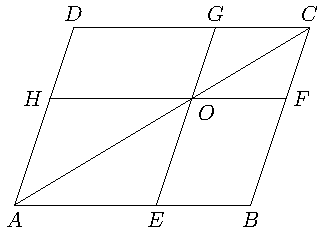
\includegraphics{pr3-17-5.pdf}
      \caption*{第 \ref{prac:3-17-5} 题}
    \end{minipage}
  \end{figurehere}
  \item 求作一个五边形和已知五边形相似,并且相似比等于 2.5。
  \item 求作一个五边形和已知五边形位似,并且位似比等于 $-\dfrac{3}{2}$。
\end{question}
\end{Practice}

\subsection{相似测量}
\subsubsection{测量地面上中间有障碍物的两点间距离}
要测量地面上中间有障碍物的 $A$、$B$ 两点间的距离(图3.117),可以按照下面的步骤进行。

\begin{enumerate}
    \item 在地面上选择适当的一点$C$作为测站(要使从$C$到
$A$,从$C$到$B$的距离可以直接量得),在$A$、$B$两点各插一根
标杆,把平板仪放在$C$点,使平板成水平,把地面上的$C$点
用移点器移到固定在平板上的图纸上,得到$C$点的对应点
$C'$,在$C'$点插一根小针。
\item 在平板上,把照准器的尺的边靠紧插在$C'$点的小
针,照准地面上$CA$和$CB$的方向,在图纸上描出对应的方向
线。
\item 量出$\overline{CA}$和$\overline{CB}$的实距长度,按照预定的比例尺
缩小,在图纸上按照缩小后的长度,分别在对应的方向线上
截取线段$\overline{C'A'}$和$\overline{C'B'}$,定出$A'$、$B'$两点。
\item 量出图纸上$\overline{A'B'}$的长度,再按照原来预定的比例
尺把$\overline{A'B'}$的长度放大,若放大率(即比例尺)等于$k$,则
$\overline{AB}=\frac{1}{k}\overline{A'B'}$。
\end{enumerate}

\begin{figure}
    \centering
% \includegraphics[scale=.6]{fig/3-117.png}
    \caption{}
\end{figure}

\subsubsection{测绘具有多边形形状地段的平面图}
要测绘多边形$ABCDE$形状地块的平面(图3.118),
可以按照下面的步骤进行。

\begin{figure}
    \centering
\begin{tikzpicture}[>=latex]
% \tkzDefPoint(0,0){S'}
% \tkzDefPoint(-150:1){A'}
% \tkzDefPoint(-35:1.1){B'}
% \tkzDefPoint(60:1.5){C'}
% \tkzDefPoint(100:.8){D'}
% \tkzDefPoint(135:1.6){E'}
% \tkzDefPointWith[linear, K=3.5](S',A') \tkzGetPoint{A}
% \tkzDefPointWith[linear, K=3.5](S',B') \tkzGetPoint{B}
% \tkzDefPointWith[linear, K=3.5](S',C') \tkzGetPoint{C}
% \tkzDefPointWith[linear, K=3.5](S',D') \tkzGetPoint{D}
% \tkzDefPointWith[linear, K=3.5](S',E') \tkzGetPoint{E}

% \tkzDrawPolygon(A,B,C,D,E)
% \tkzDrawPolygon(A',B',C',D',E')
% \tkzDrawSegments[dashed](S',A S',B S',C S',D S',E)
% \tkzLabelPoints[above](C,D,E,C',D',E')
% \tkzLabelPoints[below](A,B,A',B')
% \tkzLabelPoints[right](S')

% \draw[thick](-2.3,-1.2) rectangle (1.8,2);

\end{tikzpicture}
    \caption{}
\end{figure}


\begin{enumerate}
    \item 把平板仪放在地面上的适当一点$S$,要从$S$能直接
看到插在多边形各顶点的标杆,并且在$S$点能直接量得从$S$
到各顶点的距离,使平板成水平,平板上放图纸,把地面
上的$S$点用移点器移到图纸上,得到$S$点的对应点$S'$(图
上$S$和$S'$重合),在$S'$点插一根小针。

\item 在图纸上,划出和地面上$SA,SB,SC,SD$和
$SE$方向相同的射线。
\item 在地面上测量出$\overline{SA}$、$\overline{SB}$、$\overline{SC}$、$\overline{SD}$和$\overline{SE}$各线段
的实际长度,并且按照预定的比例尺缩小成线段$\overline{S'A'}$、
$\overline{S'B'}$、$\overline{S'C'}$、$\overline{S'D'}$和$\overline{S'E'}$,然后在图纸上各条对应的方
向射线上分别截得$\overline{S'A'}$、$\overline{S'B'}$、$\overline{S'C'}$、$\overline{S'D'}$和$\overline{S'E'}$,再
作$\overline{A'B'}$、$\overline{B'C'}$、$\overline{C'D'}$、$\overline{D'E'}$、$\overline{E'A'}$,所得多边形
$A'B'C'D'E'$就是地面上多边形$ABCDE$按照预定比例尺
缩小的平面图。
\end{enumerate}

要计算多边形$ABCDE$的面积,可先计算出平面图形
$A'B'C'D'E'$的面积,然后乘以原比例尺的平方的倒数,
算出实际地块的面积。


\subsection*{实习作业}
\begin{enumerate}
    \item 在田野里选择有障碍物的两点(如两棵树),用这节介绍
    的方法测量它们之间的距离。
    \item 选择一块多边形空地,测绘它的平面图并求出它的面积。
\end{enumerate}

\section*{习题3.5}
\addcontentsline{toc}{subsection}{习题3.5}
\begin{enumerate}
    \item 在$\triangle ABC$中,已知$\overline{BC}=36$cm, 高$\overline{AD}=30$cm, 在距
    离$\overline{BC}$边10cm的地方作一条平行于$BC$的直线,交$\overline{AB}$
    于$E$,交$\overline{AC}$于$F$,求$\overline{EF}$的长。
    \item 已知梯形两底的长为36cm和60cm, 高为32cm, 求这个梯
    形两腰延长线的交点到两底的距离各是多少?
    \item 两个相似三角形对应边的比是$7:5$,第一个三角形的周长
    是14cm, 求另一个三角形的周长。
    \item 已知$\triangle ABC\sim \triangle A'B'C$,$\triangle A'B'C'$的面积是$\triangle ABC$
    面积的4倍,并且$\overline{AB}=4$cm, $\overline{BC}=7$cm, $\overline{AC}=8$cm, 求
    $\triangle A'B'C'$各边的长。
    \item 已知梯形$ABCD$的面积为90平方厘米,两底$\overline{AB}$、$\overline{CD}$的长各
    为12厘米和8厘米,延长梯形两腰相交于$M$点,求$\triangle MDC$
    的面积。
    \item 设$AD$是$\triangle ABC$的中线,一条与
    $\overline{BC}$边平行的直线与
    $\overline{AB}$、$\overline{AD}$、$\overline{AC}$的交点分别为$P$、$Q$、$R$,那么$\overline{PQ}=\overline{QR}$
    \item 过梯形$ABCD$的对角线$AC$、$BD$的交点$E$,作两底的平
    行线,与两腰$\overline{AB}$、$\overline{CD}$分别相交于$M$、$N$,求证:
    $\overline{ME}=\overline{EN}$。
    \item 在梯形$ABCD$中,作与两底互相平行的直线,交两腰
    $\overline{AB}$、$\overline{CD}$于$P$、$Q$两点,与对角线的交点是$R$、$S$,那么
    $\overline{PR}=\overline{SQ}$
\end{enumerate}

\begin{figure}
    \begin{minipage}[t]{0.48\linewidth}
    \centering
\begin{tikzpicture}[>=latex, scale=1]
%     \tkzDefPoints{-2/0/B, 2/0/C, 1/2.5/D, -1/2.5/A}
%     \tkzInterLL(A,C)(B,D)  \tkzGetPoint{E}
% \tkzDrawSegments(A,C B,D)
% \tkzDrawPolygon(A,B,C,D)

% \tkzDefPointWith[linear, K=.3333](A,B)  \tkzGetPoint{M}
% \tkzDefPointWith[linear, K=.3333](D,C)  \tkzGetPoint{N}
% \tkzLabelPoints[left](A,B,M)
% \tkzLabelPoints[right](C,D,N)
% \tkzLabelPoints[below](E)
% \tkzDrawSegments(M,N)
    \end{tikzpicture}
    \caption*{第7题}
    \end{minipage}
    \begin{minipage}[t]{0.48\linewidth}
    \centering
    \begin{tikzpicture}[>=latex, scale=1]
%         \tkzDefPoints{-2/0/B, 2/0/C, 1/2.5/D, -1/2.5/A}
%     \tkzDrawSegments(A,C B,D)
%     \tkzDrawPolygon(A,B,C,D)

% \tkzDefPointWith[linear, K=.7](A,B)  \tkzGetPoint{P}
% \tkzDefPointWith[linear, K=.7](D,C)  \tkzGetPoint{Q}
% \tkzInterLL(A,C)(P,Q)  \tkzGetPoint{S}
% \tkzInterLL(P,Q)(B,D)  \tkzGetPoint{R}
% \tkzLabelPoints[below](R,S)
% \tkzLabelPoints[left](A,B,P)
% \tkzLabelPoints[right](C,D,Q)
% \tkzDrawSegments(P,Q)
    \end{tikzpicture}
    \caption*{第8题}
    \end{minipage}
    \end{figure}

\section*{复习题三}
\addcontentsline{toc}{section}{复习题三}
\begin{enumerate}
    \item 已知不共线三点,能不能作一个等边三角形,使这三个
    点分别在三边上?
    \item 求证:三角形的三条角平分线相交于一点。
    \item 求证:等腰三角形底边上任意一点到两腰的距离的和一
    定。它等于什么?如果在底边的延长线上取点,你能得出
    合什么结论?
    \item $O$点是等边三角形内任一点,试证明:$O$点到三边距离的
    和与$O$点的位置无关,这个和等于什么?
    \item 已知四边形,求这样一点,使这点到各顶点的距离的和
    为最小。
    \item 已知梯形$ABCD$中,$\overline{AD}\parallel\overline{BC}$,$\angle B=\ang{90}$,
    $\angle C=\ang{60}$,腰$\overline{CD}=42$cm, 求另一腰$\overline{AB}$等于多少厘米?
    \item 从平行四边形$ABCD$的各顶点到形外一条直线作垂线
    $AE$、$BF$,$CG$、$DH$,设$E$、$F$、$G$、$H$为垂足。求证:
    $\overline{AE}+\overline{CG}=\overline{BF}+\overline{DH}$。
    \item 如果两正方形对角线相等,那么这两个正方形全等。
\item 已知一边和一条对角线,求作矩形。
\item 已知高,求作等边三角形。
\item 如图,$DE\parallel BC$,$BE$、$CD$相交于$F$,射线$AF$和$\overline{BC}$
相交于$G$。求证:$\overline{BG}=\overline{CG}$。
\item 如图,已知:$\triangle ABC$中$DE\parallel CA$,$DF\parallel BA$。

求证:$\frac{\overline{DE}}{\overline{AC}}+\frac{\overline{DF}}{\overline{AB}}=1$

\begin{figure}
    \begin{minipage}[t]{0.48\linewidth}
    \centering
\begin{tikzpicture}[>=latex, scale=1]
% \tkzDefPoints{0/0/B, 4/0/C, 3/3.5/A}
% \tkzDefPointWith[linear, K=.6](A,B)  \tkzGetPoint{D}
% \tkzDefPointWith[linear, K=.6](A,C)  \tkzGetPoint{E}
% \tkzDrawPolygon(A,B,C)
% \tkzDrawSegments(D,E C,D B,E)
% \tkzInterLL(C,D)(B,E)  \tkzGetPoint{F}
% \tkzInterLL(A,F)(B,C)  \tkzGetPoint{G}
% \tkzDrawSegments(A,G)
% \tkzLabelPoints[left](D,B)
% \tkzLabelPoints[right](E,C,F)
% \tkzLabelPoints[below](G)
% \tkzLabelPoints[above](A)
    \end{tikzpicture}
    \caption*{第11题}
    \end{minipage}
    \begin{minipage}[t]{0.48\linewidth}
    \centering
    \begin{tikzpicture}[>=latex, scale=1]
%         \tkzDefPoints{0/0/B, 4/0/C, 1.5/3/A}
%         \tkzDrawPolygon(A,B,C)
%         \tkzDefPointWith[linear, K=.6](A,B)  \tkzGetPoint{E}
%         \tkzDefPointWith[linear, K=.6](C,A)  \tkzGetPoint{F}
%         \tkzDefPointWith[linear, K=.6](C,B)  \tkzGetPoint{D}
% \tkzDrawSegments(D,E D,F)
% \tkzLabelPoints[below](B,C,D)
% \tkzLabelPoints[left](E)
% \tkzLabelPoints[right](F)
% \tkzLabelPoints[above](A)
    \end{tikzpicture}
    \caption*{第12题}
    \end{minipage}
    \end{figure}

\item 已知:$D$、$D'$是$\triangle ABC$的$\overline{BC}$边上两点,$\overline{BD}=\overline{D'C}$,
$\overline{DE}$,$\overline{D'E'}$和$\overline{AC}$平行,并交$\overline{AB}$于$E,E'$,$\overline{DF}$,$\overline{D'F'}$ 和$AB$
平行交$\overline{AC}$于$F$、$F'$,求证:$E'F\parallel EF'$。
\item 已知:$E$是正方形$ABCD$的$\overline{AB}$边上的一点,
$\overline{AE}=\frac{1}{n}\overline{AB}$,$\overline{DE}$和$\overline{AC}$相交于$F$。求证;$\overline{AF}=\frac{1}{n+1}\overline{AC}$。
\item 如图,已知 $\overline{EF}\parallel \overline{BC}$,$\overline{FD}\parallel\overline{AB}$,$\overline{AE}=6.4$厘米,
$\overline{BE}=7.2$厘米,$\overline{CD}=9$厘米,
求四边形$BDFE$的周长。
\item 已知$\triangle ABC$的三边是
$\overline{AB}=11$cm, $\overline{BC}=6$cm,
$\overline{AC}=7$cm, $\overline{AD}$,$\overline{AD'}$分别是$\angle A$和它的外角平分线,求
$\overline{DD'}$的长。
\item 已知$P$是$\angle A$内的一个定点,求经过$P$作一条直线,分
别交$\angle A$的两边于$B$、$C$,使$\overline{AB}:\overline{AC}=3:2$。
\item $OC$是$\angle AOB$内的一条射线,求证从$OC$上任意两 点到 $\angle AOB$ 的两边的距离的比一定。

\begin{figure}
    \begin{minipage}[t]{0.48\linewidth}
    \centering
\begin{tikzpicture}[>=latex, scale=1]
% \tkzDefPoints{0/0/B, 4/0/C, 2.3/2/A}
% \tkzDefPointWith[linear, K=.4](A,B) \tkzGetPoint{E}
% \tkzDefPointWith[linear, K=.4](A,C) \tkzGetPoint{F}
% \tkzDefPointWith[linear, K=.6](C,B) \tkzGetPoint{D}
% \tkzDrawPolygon(A,B,C)
% \tkzDrawSegments(E,F D,F)
% \tkzLabelPoints[below](B,C,D)
% \tkzLabelPoints[left](E)
% \tkzLabelPoints[right](F)
% \tkzLabelPoints[above](A)
    \end{tikzpicture}
    \caption*{第15题}
    \end{minipage}
    \begin{minipage}[t]{0.48\linewidth}
    \centering
    \begin{tikzpicture}[>=latex, scale=1]
% \tkzDefPoints{0/0/B, 4/0/C, 3/3/A}
% \tkzDefPointWith[linear, K=.45](A,B) \tkzGetPoint{D}
% \tkzDefPointWith[linear, K=.55](A,C) \tkzGetPoint{F}
% \tkzDefPointWith[linear, K=.45](C,B) \tkzGetPoint{E}
% \tkzDrawPolygon(A,B,C)
% \tkzDrawSegments(E,F D,E)
% \tkzLabelPoints[below](B,C,E)
% \tkzLabelPoints[left](D)
% \tkzLabelPoints[right](F)
% \tkzLabelPoints[above](A)
    \end{tikzpicture}
    \caption*{第19题}
    \end{minipage}
    \end{figure}

\item 如图,$D$、$E$、$F$分别是$\triangle ABC$的边$\overline{AB}$、$\overline{BC}$、$\overline{CA}$
上的点,$ADEF$
是菱形,$\overline{AB}=14$cm, $\overline{BC}=12$cm, $\overline{AC}=10$cm, 求$\overline{BE}$和$\overline{EC}$
的长。

\item 已知:$E$是平行四边形
$ABCD$的边$\overline{DA}$延长线上的一点,$\overline{EC}$交$\overline{AB}$于$G$,交对角线$\overline{DB}$于$F$。

求证:$\overline{FC}^2=\overline{FG}\cdot \overline{FE}$
\item 设$\overline{AB}$的中点为$M$,从$\overline{AB}$上另一点$C$向直线$AB$的一
侧引线段$\overline{CD}$。令$\overline{CD}$的中点为$N$,$\overline{BD}$的中点为$P$,$\overline{MN}$
的中点为$Q$,求证:直线$PQ$平分$\overline{AC}$。
\item 已知梯形的面积是$Q$,上下底的比是$\frac{m}{n}$,
求两腰的延长线和上底所组成的三角形的面积。
\item 在直角三角形$ABC$中,$\overline{AD}$是斜边$\overline{BC}$上的高,作
$DE\perp AB$,$DF\perp AC$,$E,F$是垂足.

求证:$\frac{\overline{BE}}{\overline{CF}}=\frac{\overline{AC}^3}{\overline{AB}^3}$

\item 如图,已知$\overline{OM}:\overline{MP}=\overline{ON}:\overline{NR}$,
求证:$\triangle PQR$是等腰三角形。

\begin{figure}
    \begin{minipage}[t]{0.48\linewidth}
    \centering
\begin{tikzpicture}[>=latex, scale=.8]
% \tkzDefPoints{0/0/O, 3/0/R, 4/3/N}
% \tkzDefPointWith[linear, K=.4](O,N) \tkzGetPoint{M}
% \tkzDefPointWith[linear, K=1.6](N,R) \tkzGetPoint{Q}
% \tkzInterLL(O,R)(M,Q)  \tkzGetPoint{P}
% \tkzLabelPoints[right](N,R,Q)
% \tkzLabelPoints[left](O,M)
% \tkzLabelPoints[below](P)
% \tkzDrawPolygon(O,N,R)
% \tkzDrawPolygon(N,Q,M)
    \end{tikzpicture}
    \caption*{第24题}
    \end{minipage}
    \begin{minipage}[t]{0.48\linewidth}
    \centering
    \begin{tikzpicture}[>=latex, scale=1]
% \tkzDefPoints{0/0/B, 3/0/C, 2.4/3.5/A, 5/0/X, 4/.5/X1}
% \tkzInterLL(X,X1)(A,C)  \tkzGetPoint{Y}
% \tkzInterLL(X,X1)(A,B)  \tkzGetPoint{Z}
% \tkzDrawPolygon(A,B,C)
% \tkzDrawPolygon(X,B,Z)
% \tkzLabelPoints[right](Y)
% \tkzLabelPoints[left](A,Z)
% \tkzLabelPoints[below](B,C,X)
    \end{tikzpicture}
    \caption*{第25题}
    \end{minipage}
    \end{figure}

\item $\triangle ABC$被一条直线所截,设与三边的交点为$X$、$Y$、$Z$,

试证:$\frac{\overline{BX}}{\overline{XC}}\cdot \frac{\overline{CY}}{\overline{YA}}\cdot \frac{\overline{AZ}}{\overline{ZB}}=1$

\item 设$O$是$\triangle ABC$内任一点,射线$AO$、$BO$、$CO$与对边的交点分别是$X$、$Y$、$Z$,那么
$\frac{\overline{BX}}{\overline{XC}}\cdot \frac{\overline{CY}}{\overline{YA}}\cdot \frac{\overline{AZ}}{\overline{ZB}}=1$


\begin{figure}
    \begin{minipage}[t]{0.48\linewidth}
    \centering
\begin{tikzpicture}[>=latex, scale=1]
%     \tkzDefPoints{0/0/B, 4/0/C, 2.9/3.2/A, 2.5/1.5/O}
% \tkzInterLL(A,O)(B,C)  \tkzGetPoint{X}
% \tkzInterLL(B,O)(A,C)  \tkzGetPoint{Y}
% \tkzInterLL(C,O)(B,A)  \tkzGetPoint{Z}
% \tkzDrawPolygon(A,B,C)
% \tkzDrawSegments(A,X B,Y C,Z)
% \tkzLabelPoints[right](Y)
% \tkzLabelPoints[left](A,Z)
% \tkzLabelPoints[below](B,C,X)
% \tkzLabelPoints[below left](O)
    \end{tikzpicture}
    \caption*{第26题}
    \end{minipage}
    \begin{minipage}[t]{0.48\linewidth}
    \centering
    \begin{tikzpicture}[>=latex, scale=1]
% \tkzDefPoints{0/0/B, 2.6/0/C, 2.4/3.5/A, 5/0/D, 4/.25/X1}
% \tkzInterLL(D,X1)(A,C)  \tkzGetPoint{E}
% \tkzInterLL(D,X1)(A,B)  \tkzGetPoint{F}
% \tkzDrawPolygon(A,B,C)
% \tkzDrawPolygon(D,B,F)
% \tkzLabelPoints[right](E)
% \tkzLabelPoints[left](A,F)
% \tkzLabelPoints[below](B,C,D)      
    \end{tikzpicture}
    \caption*{第27题}
    \end{minipage}
    \end{figure}

\item 从$\triangle ABC$的一边$\overline{BC}$的延长线上的一点$D$,引直线与
其它二边$\overline{AC}$、$\overline{AB}$相交于$E$、$F$,若$\angle AEF=\angle AFE$,则$\overline{BD}:\overline{CD}=\overline{BF}:\overline{CE}$。


\item 在$\triangle ABC$之边$\overline{AB}$、$\overline{AC}$上取$E$、$F$两点,使$\overline{EB}=2\overline{EA}$,$\overline{AF}=2\overline{FC}$,延长$\overline{EF}$、$\overline{BC}$交于$H$,求$\overline{BH}:\overline{CH}$。

\begin{figure}
    \begin{minipage}[t]{0.48\linewidth}
    \centering
\begin{tikzpicture}[>=latex, scale=1]
%     \tkzDefPoints{0/0/B, 4/0/C, 3/3/A}
% \tkzDefPointWith[linear, K=0.333](A,B) \tkzGetPoint{E}
% \tkzDefPointWith[linear, K=0.333](C,A) \tkzGetPoint{F}
% \tkzInterLL(B,C)(E,F)  \tkzGetPoint{H}
% \tkzDrawPolygon(A,B,C)
% \tkzDrawSegments(E,H C,H)
% \tkzLabelPoints[right](F)
% \tkzLabelPoints[left](A,E)
% \tkzLabelPoints[below](B,C,H)  
    \end{tikzpicture}
    \caption*{第28题}
    \end{minipage}
    \begin{minipage}[t]{0.48\linewidth}
    \centering
    \begin{tikzpicture}[>=latex, scale=1]
%         \tkzDefPoints{0/0/A, 2/0/B, 4/0/D, 2.8/3/C}
% \tkzDrawPolygon(A,B,C)
% \tkzDefPointWith[linear, K=.45](C,A) \tkzGetPoint{E}
% \tkzInterLL(D,E)(B,C)  \tkzGetPoint{F}
% \tkzLabelPoints[right](F)
% \tkzLabelPoints[left](C,E)
% \tkzLabelPoints[below](B,A,D)  
% \tkzDrawSegments(E,D B,D)
    \end{tikzpicture}
    \caption*{第29题}
    \end{minipage}
    \end{figure}

\item 在$\triangle ABC$中,$\overline{AB}<\overline{AC}$,延长$\overline{AB}$至$D$,使$\overline{BD}=\overline{AB}$,在$\overline{AC}$上取$E$点,使$\overline{CE}=\overline{BD}$,连接$\overline{DE}$与$\overline{BC}$交于 $F$,则$\overline{AB}:\overline{AC}=\overline{EF}:\overline{FD}$。
\item 延长$\triangle ABC$的$\overline{BC}$边至$D$,使$\overline{CD}=\overline{BC}$,从$D$点引直线通过$\overline{AC}$的中点$E$,与$\overline{AB}$边相交于$F$,求$\overline{FE}:\overline{ED}$。
\item 从$\triangle ABC$的底边$\overline{BC}$中点$D$引直线,与过顶点$A$平行$BC$的直线相交于$G$,与$\overline{BA}$的延长线相交于$E$,又与$AC$相交于$F$,求证:$\overline{DF}:\overline{FG}=\overline{DE}:\overline{EG}$。

\begin{figure}
    \begin{minipage}[t]{0.48\linewidth}
    \centering
\begin{tikzpicture}[>=latex, scale=1]
    % \tkzDefPoints{0/0/B, 2/0/C, 4/0/D, 2.2/3.5/A}
    % \tkzDrawPolygon(A,B,C)
    % \tkzDefMidPoint(A,C)  \tkzGetPoint{E}
    % \tkzInterLL(D,E)(B,A)  \tkzGetPoint{F}
    % \tkzLabelPoints[right](E)
    % \tkzLabelPoints[left](A,F)
    % \tkzLabelPoints[below](B,C,D)   
    % \tkzDrawSegments(C,D D,F)
    \end{tikzpicture}
    \caption*{第30题}
    \end{minipage}
    \begin{minipage}[t]{0.48\linewidth}
    \centering
    \begin{tikzpicture}[>=latex, scale=.8]
    % \tkzDefPoints{0/0/B, 2/0/D, 4/0/C, 1.6/2.5/A, 3.5/2.5/X1, 2.2/1/X2}
    % \tkzDrawPolygon(A,B,C)
    % \tkzInterLL(D,X2)(B,A)  \tkzGetPoint{E}
    % \tkzInterLL(D,X2)(X1,A)  \tkzGetPoint{G}
    % \tkzInterLL(D,X2)(C,A)  \tkzGetPoint{F}
    % \tkzLabelPoints[right](F)
    % \tkzLabelPoints[left](A,E)
    % \tkzLabelPoints[above right](G)
    % \tkzLabelPoints[below](B,C,D)   
    % \tkzDrawSegments(A,X1 A,E E,D)
    \end{tikzpicture}
    \caption*{第31题}
    \end{minipage}
    \end{figure}
\end{enumerate}